% Options for packages loaded elsewhere
\PassOptionsToPackage{unicode}{hyperref}
\PassOptionsToPackage{hyphens}{url}
%
\documentclass[
]{book}
\usepackage{amsmath,amssymb}
\usepackage{iftex}
\ifPDFTeX
  \usepackage[T1]{fontenc}
  \usepackage[utf8]{inputenc}
  \usepackage{textcomp} % provide euro and other symbols
\else % if luatex or xetex
  \usepackage{unicode-math} % this also loads fontspec
  \defaultfontfeatures{Scale=MatchLowercase}
  \defaultfontfeatures[\rmfamily]{Ligatures=TeX,Scale=1}
\fi
\usepackage{lmodern}
\ifPDFTeX\else
  % xetex/luatex font selection
\fi
% Use upquote if available, for straight quotes in verbatim environments
\IfFileExists{upquote.sty}{\usepackage{upquote}}{}
\IfFileExists{microtype.sty}{% use microtype if available
  \usepackage[]{microtype}
  \UseMicrotypeSet[protrusion]{basicmath} % disable protrusion for tt fonts
}{}
\makeatletter
\@ifundefined{KOMAClassName}{% if non-KOMA class
  \IfFileExists{parskip.sty}{%
    \usepackage{parskip}
  }{% else
    \setlength{\parindent}{0pt}
    \setlength{\parskip}{6pt plus 2pt minus 1pt}}
}{% if KOMA class
  \KOMAoptions{parskip=half}}
\makeatother
\usepackage{xcolor}
\usepackage{color}
\usepackage{fancyvrb}
\newcommand{\VerbBar}{|}
\newcommand{\VERB}{\Verb[commandchars=\\\{\}]}
\DefineVerbatimEnvironment{Highlighting}{Verbatim}{commandchars=\\\{\}}
% Add ',fontsize=\small' for more characters per line
\usepackage{framed}
\definecolor{shadecolor}{RGB}{248,248,248}
\newenvironment{Shaded}{\begin{snugshade}}{\end{snugshade}}
\newcommand{\AlertTok}[1]{\textcolor[rgb]{0.94,0.16,0.16}{#1}}
\newcommand{\AnnotationTok}[1]{\textcolor[rgb]{0.56,0.35,0.01}{\textbf{\textit{#1}}}}
\newcommand{\AttributeTok}[1]{\textcolor[rgb]{0.13,0.29,0.53}{#1}}
\newcommand{\BaseNTok}[1]{\textcolor[rgb]{0.00,0.00,0.81}{#1}}
\newcommand{\BuiltInTok}[1]{#1}
\newcommand{\CharTok}[1]{\textcolor[rgb]{0.31,0.60,0.02}{#1}}
\newcommand{\CommentTok}[1]{\textcolor[rgb]{0.56,0.35,0.01}{\textit{#1}}}
\newcommand{\CommentVarTok}[1]{\textcolor[rgb]{0.56,0.35,0.01}{\textbf{\textit{#1}}}}
\newcommand{\ConstantTok}[1]{\textcolor[rgb]{0.56,0.35,0.01}{#1}}
\newcommand{\ControlFlowTok}[1]{\textcolor[rgb]{0.13,0.29,0.53}{\textbf{#1}}}
\newcommand{\DataTypeTok}[1]{\textcolor[rgb]{0.13,0.29,0.53}{#1}}
\newcommand{\DecValTok}[1]{\textcolor[rgb]{0.00,0.00,0.81}{#1}}
\newcommand{\DocumentationTok}[1]{\textcolor[rgb]{0.56,0.35,0.01}{\textbf{\textit{#1}}}}
\newcommand{\ErrorTok}[1]{\textcolor[rgb]{0.64,0.00,0.00}{\textbf{#1}}}
\newcommand{\ExtensionTok}[1]{#1}
\newcommand{\FloatTok}[1]{\textcolor[rgb]{0.00,0.00,0.81}{#1}}
\newcommand{\FunctionTok}[1]{\textcolor[rgb]{0.13,0.29,0.53}{\textbf{#1}}}
\newcommand{\ImportTok}[1]{#1}
\newcommand{\InformationTok}[1]{\textcolor[rgb]{0.56,0.35,0.01}{\textbf{\textit{#1}}}}
\newcommand{\KeywordTok}[1]{\textcolor[rgb]{0.13,0.29,0.53}{\textbf{#1}}}
\newcommand{\NormalTok}[1]{#1}
\newcommand{\OperatorTok}[1]{\textcolor[rgb]{0.81,0.36,0.00}{\textbf{#1}}}
\newcommand{\OtherTok}[1]{\textcolor[rgb]{0.56,0.35,0.01}{#1}}
\newcommand{\PreprocessorTok}[1]{\textcolor[rgb]{0.56,0.35,0.01}{\textit{#1}}}
\newcommand{\RegionMarkerTok}[1]{#1}
\newcommand{\SpecialCharTok}[1]{\textcolor[rgb]{0.81,0.36,0.00}{\textbf{#1}}}
\newcommand{\SpecialStringTok}[1]{\textcolor[rgb]{0.31,0.60,0.02}{#1}}
\newcommand{\StringTok}[1]{\textcolor[rgb]{0.31,0.60,0.02}{#1}}
\newcommand{\VariableTok}[1]{\textcolor[rgb]{0.00,0.00,0.00}{#1}}
\newcommand{\VerbatimStringTok}[1]{\textcolor[rgb]{0.31,0.60,0.02}{#1}}
\newcommand{\WarningTok}[1]{\textcolor[rgb]{0.56,0.35,0.01}{\textbf{\textit{#1}}}}
\usepackage{longtable,booktabs,array}
\usepackage{calc} % for calculating minipage widths
% Correct order of tables after \paragraph or \subparagraph
\usepackage{etoolbox}
\makeatletter
\patchcmd\longtable{\par}{\if@noskipsec\mbox{}\fi\par}{}{}
\makeatother
% Allow footnotes in longtable head/foot
\IfFileExists{footnotehyper.sty}{\usepackage{footnotehyper}}{\usepackage{footnote}}
\makesavenoteenv{longtable}
\usepackage{graphicx}
\makeatletter
\def\maxwidth{\ifdim\Gin@nat@width>\linewidth\linewidth\else\Gin@nat@width\fi}
\def\maxheight{\ifdim\Gin@nat@height>\textheight\textheight\else\Gin@nat@height\fi}
\makeatother
% Scale images if necessary, so that they will not overflow the page
% margins by default, and it is still possible to overwrite the defaults
% using explicit options in \includegraphics[width, height, ...]{}
\setkeys{Gin}{width=\maxwidth,height=\maxheight,keepaspectratio}
% Set default figure placement to htbp
\makeatletter
\def\fps@figure{htbp}
\makeatother
\setlength{\emergencystretch}{3em} % prevent overfull lines
\providecommand{\tightlist}{%
  \setlength{\itemsep}{0pt}\setlength{\parskip}{0pt}}
\setcounter{secnumdepth}{5}
\usepackage{booktabs}
\usepackage{amsthm}
\makeatletter
\def\thm@space@setup{%
  \thm@preskip=8pt plus 2pt minus 4pt
  \thm@postskip=\thm@preskip
}
\makeatother
\ifLuaTeX
  \usepackage{selnolig}  % disable illegal ligatures
\fi
\usepackage[]{natbib}
\bibliographystyle{apalike}
\IfFileExists{bookmark.sty}{\usepackage{bookmark}}{\usepackage{hyperref}}
\IfFileExists{xurl.sty}{\usepackage{xurl}}{} % add URL line breaks if available
\urlstyle{same}
\hypersetup{
  pdftitle={NIRS Study Information},
  pdfauthor={Sara Grace Biddle},
  hidelinks,
  pdfcreator={LaTeX via pandoc}}

\title{NIRS Study Information}
\author{Sara Grace Biddle}
\date{2024-01-19}

\begin{document}
\maketitle

{
\setcounter{tocdepth}{1}
\tableofcontents
}
\hypertarget{about}{%
\chapter{About}\label{about}}

This study is being conducted in collaboration with the PrismaHealth Cancer Institute, Furman University Health Science Department, and University of South Carolina School of Medicine Greenville.

\hypertarget{contact-information}{%
\section{Contact Information}\label{contact-information}}

\begin{center}\rule{0.5\linewidth}{0.5pt}\end{center}

\textbf{Dr.~Jennifer Trilk}

\begin{quote}
Principal Investigator\\
University of South Carolina School of Medicine- Greenville\\
\href{mailto:trilk@greenvillemed.sc.edu}{\nolinkurl{trilk@greenvillemed.sc.edu}}
\end{quote}

\textbf{Dr.~Randolph Hutchison}

\begin{quote}
Principal Investigator\\
Furman University Department of Health Science\\
\href{mailto:randolph.hutchison@furman.edu}{\nolinkurl{randolph.hutchison@furman.edu}}
\end{quote}

\textbf{Dr.~Larry Gluck}

\begin{quote}
\href{mailto:Larry.Gluck@prismahealth.org}{\nolinkurl{Larry.Gluck@prismahealth.org}}
\end{quote}

\textbf{Dr.~Julie Martin}

\begin{quote}
Director of Cancer Research\\
Prisma Health\\
\href{mailto:Julie.Martin@prismahealth.org}{\nolinkurl{Julie.Martin@prismahealth.org}}
\end{quote}

\textbf{Frankie Bennett}

\begin{quote}
Human Performance Lab Coordinator\\
University of South Carolina School of Medicine- Greenville\\
\href{mailto:BENNETT24@greenville.sc.edu}{\nolinkurl{BENNETT24@greenville.sc.edu}}
\end{quote}

\textbf{Sara Biddle}

\begin{quote}
Research Coordinator\\
Prisma Health Cancer Institute\\
\href{mailto:sara.biddle@prismahealth.org}{\nolinkurl{sara.biddle@prismahealth.org}}
\end{quote}

\textbf{Sydney Hackwell}

\begin{quote}
Research Coordinator\\
Prisma Health Cancer Institute\\
\href{mailto:sydney.hackwell@prismahealth.org}{\nolinkurl{sydney.hackwell@prismahealth.org}}
\end{quote}

\textbf{Katie Banenas}

\begin{quote}
Research Coordinator\\
Prisma Health Cancer Institute\\
\href{mailto:katie.banenas@prismahealth.org}{\nolinkurl{katie.banenas@prismahealth.org}}
\end{quote}

\textbf{Human Performance Lab}

\begin{quote}
\begin{enumerate}
\def\labelenumi{(\arabic{enumi})}
\setcounter{enumi}{863}
\tightlist
\item
  455-1410
\end{enumerate}
\end{quote}

\hypertarget{Literature}{%
\chapter{Literature}\label{Literature}}

\hypertarget{Literature-nirs}{%
\section{Near Infrared Spectrosopy}\label{Literature-nirs}}

Continuous wave NIRS devices use the modified Beer-Lambert law to calculate the volume of oxygenated and deoxygenated hemoglobin.

Spatially resolved NIRS devices use multiple transmitters at different distances from a reciever to calculate a Tissue Saturation Index, or TSI.

The NIRS device utilized in this study is the PortaMon by Artinis Medical Systems. The PortaMon could be considered both a continuous wave and spatially resolved device. It uses three continuous-wave transmitters with a single receiver to calculate the TSI.

Each transmitter emits two wavelengths of infrared light. One wavelength is for oxygenated hemoglobin and one wavelength is for deoxygenated hemoglobin, therefore each transmitter measures both oxygenated and deoxygenated hemoglobin.

The transmitters emit light into tissue where the light waves bounce off structures in the tissue and return to the receiver.

The receiver measures the light that returns in Optical Densities. Calculations using several different parameters and assumptions convert OD into usable units.

Subcutaneous adipose tissue has different optical properties than muscle tissue. Most calculations do not account for two separate layers of tissue with different scattering and optical properties. There have been some papers within the last few years examining multi-layered tissues and the effects on NIRS measurements using computer modeling and phantom tissues. Most papers utilizing NIRS in exercise physiology assume a limited or negligible effect of adipose tissue thickness on measurements and report participants' adipose tissue thickness.

Different areas of the body have different types of tissue structure and this have different optical properties. Previous papers have reported the measurements of optical properties at various locations of the body. Consult with the device manufacturer and reports of these optical properties to determine the best settings for your device.

Most studies assume that the tissue structures have constant optical properties. This may not hold true, especially during activities like exercise where blood flow increases and the contents of blood fluctuate. Accounting for varying optical properties has led to the development of time-domain and other measurement techniques. These devices are more expensive than a continuous wave device. Therefore, most NIRS devices assume constant optical properties of the measured tissues.

The differential pathlength factor (dpf) is the measurement of the path that the light waves take through tissue. DPF values have been well researched and measured for multiple body locations and differing adipose tissue thicknesses. This parameter is used in calculating TSI.

\hypertarget{PatientRecruitment}{%
\chapter{Patient Recruitment}\label{PatientRecruitment}}

\hypertarget{inclusionexclusion-criteria}{%
\section{Inclusion/Exclusion Criteria}\label{inclusionexclusion-criteria}}

To be eligible for the study, patients must:

\begin{itemize}
\tightlist
\item
  have primary breast of gynecological cancer
\item
  non-metastatic
\item
  that is being treated with chemotherapy

  \begin{itemize}
  \tightlist
  \item
    no immunotherapy or radiation at the same time or before chemotherapy
  \item
    the chemotherapy regimen can be any regimen that is considered \emph{standard of care}
  \end{itemize}
\item
  cannot have had chemotherapy within the past 5 years for any reason
\item
  able to participate in moderate exercise on a stationary bike
\item
  female patients only, male breast cancer patients are not eligible at this time
\end{itemize}

\hypertarget{screening-the-electronic-medical-record}{%
\section{Screening the Electronic Medical Record}\label{screening-the-electronic-medical-record}}

Prisma Health uses EPIC as their electronic medical record service.
You can only access EPIC with permission from Prisma Health. The medical students may technically have access to EPIC but they have not had much training on how to use it and actually accessing it can be cumbersome and difficult for them. It is much easier for a Research Coordinator to do any work in EPIC.

Use the Production Environment of EPIC. In the Production Environment, you can create and run reports that you cannot in the Read Only Environment.

Log in with your Prisma Health log in information and select the department \texttt{CANCER-FARIS\ ONCOLOGY\ {[}100224000{]}}.

\hypertarget{using-a-report}{%
\subsection{Using a Report}\label{using-a-report}}

Go to \texttt{My\ Reports}.

I have a report named \texttt{NIRS\ Eligibility\ by\ Stage} that has the following parameters:

\begin{quote}
Select Patients in Registries\\
\textbf{From}\\
\emph{Registries:}\\
Registry ID: CANCER POPULATION REGISTRY\\
\emph{Level of detail:}\\
Patients

\textbf{Where}\\
\emph{Registry metrics:} (1 OR 2 OR 3 OR 4 OR 5) AND 6\\

\begin{quote}
1 Metric Name or ID: DM TREATMENT PLAN PROVIDER and Metric Value: Contains EDENFIELD, WILLIAM JEFFERY\\
2 Metric Name or ID: DM TREATMENT PLAN PROVIDER and Metric Value: Contains ELDER, JEFFERY WAYNE\\
3 Metric Name or ID: DM TREATMENT PLAN PROVIDER and Metric Value: Contains JORGENSEN, CARLA WALKER\\
4 Metric Name or ID: DM TREATMENT PLAN PROVIDER and Metric Value: Contains STEPHENSON JR, JOE JOHN\\
5 Metric Name or ID: DM TREATMENT PLAN PROVIDER and Metric Value: Contains PULS, LARRY EDWIN\\
6 Metric Name or ID: DM MED PATIENT RECIEVED CHEMOTHERAPY IN PAST YEAR and Metric Value: No\\
\end{quote}

AND \emph{Diagnosis in grouper:}\\

\begin{quote}
Diagnosis Grouper (VCG): EDG ID CANCER BREAST OR\\
Diagnosis Grouper (VCG): EDG ID CANCER FALLOPIAN TUBE OR\\
Diagnosis Grouper (VCG): EDG ID CANCER OVARY OR\\
Diagnosis Grouper (VCG): EDG ID CANCER CERVIX OR\\
Diagnosis Grouper (VCG): EDG ID CANCER VAGINA OR\\
Diagnosis Grouper (VCG): EDG ID CANCER VULVA\\
\end{quote}

AND \emph{Treatment Plan Start Date:}\\

\begin{quote}
Episode Types: Infusion Treatment and Discontinue Reasons to Exclude: (none) and Plan Number: (none) and Plan Staatuses: Active and Treatment Plan Start Date: Greater than or equal to TODAY - 14 OR\\
Episode Types: ONCOLOGY TREATMENT and Discontinue Reasons to Exlude: (none) and Plan Number: (none) and Plan Statuses: Active and Treatment Plan Start Date: Greater than or equal to TODAY - 14 OR\\
Episode Types: ONCOLOGY TREATMENT and Discontinue Reasons to Exclude: (none) and Plan Number: (none) and Plan Statuses: Future and Treatment Plan Start Date: Less than or equal to TODAY + 14 OR\\
Episode Types: Infusion Treatment and Discontinue Reasons to Exclude: (none) and Plan Number: (none) and Plan Statuses: Future and Treatment Plan Start Date: Less than or equal to TODAY + 14\\
\end{quote}

AND \emph{Cancer Stage Distant Metastasis (M) Value}:\\

\begin{quote}
Stage Classifications: Clinical and Fallback Classifications: (none) and Signed Only?: (none) and SmartData Identifier: EPIC\#42385 and Which Stage: Most Recent and Cancer Stage Distant Metastasis (M) Value: cM0 OR\\
Stage Classifications: Clinical and Fallback Classifications: (none) and Signed Only?: (none) and SmartData Identifier: EPIC\#42385 and Which Stage: Most Recent and Cancer Stage Distant Metastasis (M) Value: cM0(i+) OR\\
Stage Classifications: Clinical and Fallback Classifications: (none) and Signed Only?: (none) and SmartData Identifier: EPIC\#42385 and Which Stage: Most Recent and Cancer Stage Distant Metastasis (M) Value: M0 OR\\
Stage Classifications: Pathologic and Fallback Classifications: (none) and Signed Only?: (none) and SmartData Identifier: EPIC\#42385 and Which Stage: Most Recent and Cancer Stage Distant Metastasis (M) Value: cM0 OR\\
Stage Classifications: Pathologic and Fallback Classifications: (none) and Signed Only?: (none) and SmartData Identifier: EPIC\#42385 and Which Stage: Most Recent and Cancer Stage Distant Metastasis (M) Value: cM0(i+) OR\\
Stage Classifications: Pathologic and Fallback Classifications: (none) and Signed Only?: (none) and SmartData Identifier: EPIC\#42385 and Which Stage: Most Recent and Cancer Stage Distant Metastasis (M) Value: M0\\
\end{quote}

AND \emph{Line of Treatment}:\\

\begin{quote}
Episode Types: ONCOLOGY TREATMENT and Discontinue Reasons to Exclude: (none) and Plan Number: (none) and Plan Statuses: (none) and Line of Treatment: Not equal to Third Line OR\\
Episode Types: Infusion Treatment and Discontinue Reasons to Exclude: (none) and Plan Number: (none) and Plan Statuses: (none) and Line of Treatment: Not equal to Third Line\\
AND \emph{Treatment Plan Goal}:\\
Episode Types: Infusion Treatment and Discontinue Reasons to Exclude: (none) and Plan Number: (none) and Plan Statuses: Active and Treatment Plan Goal: Not equal to Palliative OR\\
Episode Types: Infusion Treatment and Discontinue Reasons to Exclude: (none) and Plan Number: (none) and Plan Statuses: Future and Treatment Plan Goal: Not equal to Palliative OR\\
Episode Types: ONCOLOGY TREATMENT and Discontinue Reasons to Exclude: (none) and Plan Number: (none) and Plan Statuses: Active and Treatment Plan Goal: Not equal to Palliative OR\\
Episode Types: IONCOLOGY TREATMENT and Discontinue Reasons to Exclude: (none) and Plan Number: (none) and Plan Statuses: Future and Treatment Plan Goal: Not equal to Palliative
\end{quote}
\end{quote}

This will return a list of potentially eligible patients who meet the parameters specified in the query above. I have the report settings such that the results table shows me their treatment plan start date, next oncology appointment date, name, MRN, clinical stage, diagnosis, and plan provider. When I select a patient from the list, it displays an Oncology Snapshot under the report results table. I take a quick look through the Oncolog Snapshot and if I need to take a closer look at their chart, I can open it up.

I have not figured out how to share this report or its results with other people. As it is, I look through the patients returned by the report and eliminate any definitively ineligible patients.

Sometimes metastatic disease is listed as a second diagnosis and therefore slips through the exclusion of metastatic disease. Vascular diseases and injuries that would preclude ability to exercise are other common exclusion criteria. Male patients with breast cancer are not eligible for this study. Take a quick look through the patient's problem list. If the patient does not have any immediate exclusionary problems, pass their name and MRN on to the research coordinators, Sydney Hackwell and Katie Banenas. They will conduct a full chart screening and contact the patient if they are eligible.

I include all patients returned by the report into the List. This is because, from day to day, the report returns different patients. If a patient is not in the List, I will assume that I have not yet looked at their chart. So, even if I look at a chart and immediately determine that a patient is not eligible, I write their information into the List and mark them ineligible so I don't forget that I already screened their chart. This also helps determine if there are new potentially eligible patients returned by the report. On average, the report will return between 5 and 10 patients. Due to the month long limit on treatment plan start date, the report will return the same patients for many days in a row. If you don't keep track of everyone that the report returned, even the ineligible ones, you may get confused about which patients need to be screened and which ones you have already screened.

\hypertarget{using-the-schedule}{%
\subsection{Using the Schedule}\label{using-the-schedule}}

Open the \texttt{Schedule} tab.

If there is not a schedule view that you like, you can make your own by clicking the green plus sign above \texttt{My\ Schedule}.

Give it a name. I called mine \texttt{nirs\ providers}. Under \texttt{Selected\ Columns} you can choose what information you want to display about the appointment. Under \texttt{Configuration}, you can add the providers. I added all five oncologists.

Now when you select that schedule, you will only see the five oncologists that refer to the NIRS study. To take a closer look at an appointment, expand the schedule by clicking the gray triangle next to the name of the schedule. Click on the provider name whose schedule you are interested in. This will expand the schedule of only that provider, where you can see more details about their appointments. Use the calendar in the top left to select different days.

Click on an appointment you are interested in examining further. This should open up a panel to the right of the schedule. I have this set up to show \texttt{Snapshot} as the default view. You can rearrange the panels shown in the snapshot by clicking on the wrench in the top right of the snapshot panel.

I use the schedule to screen patients coming in to the Multidisciplinary Clinic (MDC).

Jorgensen has appointments in the MDC every other Monday. Stephenson has appointments in the MDC every other Thursday. Screen these appointments at least one day before. Many will not have a chemotherapy plan or a cancer staging activity yet. Look for major health problems that would disqualify them from participation. If there are no major problems, pass the appointment information on to Katie and Sydney. If a patient has triple negative or estrogen receptor and progesterone receptor negative breast cancer, they are likely to receive chemotherapy and Katie or Sydney can contact them as soon as the chemotherapy is prescribed. This gives us more time for recruitment into the study, as Katie and Sydney can be at the MDC appointment or at the appointment where they are told about the chemotherapy, which is a lot more time than waiting until the chemo teach appointment to approach a patient.

\hypertarget{potential-patient-list}{%
\section{Potential Patient List}\label{potential-patient-list}}

I use a Microsoft List, created in my PrismaHealth OneDrive, to share the patient information with Katie and Syndey rather than sending tons of emails. I update the list when I identify potentially eligible patients. I include the patient's MRN, first and last name, primary diagnosis (breast or gynecological), and which of the referring oncologists is on their treatment team. If they have an upcoming appointment that Katie or Sydney could go to and tell them about the study, I include the appointment information. If their first chemotherapy infusion is scheduled, I include that date so that we know how long we have to recruit and schedule them in the HPL.

Katie and Sydney look through the list and conduct a more in depth chart screening. If they determine that a patient is not eligible, they click the \texttt{Ineligible} tag in the List and include reasons that the patient is not eligible. The categories of ineligibility that I included as defaults are: metastatic disease, chemotherapy treatment within the last five years, lab values, treatment plan other than chemotherapy. You can type in any new category you need; you are not limited to just the default ineligibility values.

If a patient is determined to be eligible, one of the Research Coordinators will contact their oncologist to get permission to approach the patient at their next appointment. If the provider declines the study for them, then the patient is marked as \texttt{Declined} in the List. If the provider consents for the patient to be approached about the study, then one of the Research Coordinators will approach the patient at their next appointment. The patient will then either sign a consent or decline the study. If they decline the study, click the \texttt{Declined} tag in the List. Include a reason that they declined, such as stress, not enough time, etc.

After contacting the patient, they will contact you if the patient signs the consent form. After the consent form is signed, we can begin contacting the patient to start scheduling for lab visits. Contact Dr.~Julie Martin after obtaining the consent form and she will put all NIRS related blood draws into EPIC. If for some reason we are not able to get the NIRS draws done at the same time as the other pre-chemo blood draws, consult with the patient and schedule this through Dr.~Julie Martin.

If a patient is not wearing shorts for a lab visit, there are disposable shorts in the lab for patient use. They are located in a box under the bed in the back corner.

\hypertarget{Methods}{%
\chapter{Methods}\label{Methods}}

\hypertarget{Methods-LT}{%
\section{Lactate Threshold Protocol}\label{Methods-LT}}

This protocol is the participant's first visit.

\hypertarget{Methods-LT-prep}{%
\subsection{Preparation}\label{Methods-LT-prep}}

At least 30 minutes prior to when the participant is scheduled to arrive, turn on the metabolic cart.

Print out the following instruments:

\begin{itemize}
\tightlist
\item
  MoCA \ref{Appendix-Surveys-moca}
\item
  MMSE \ref{Appendix-Surveys-mmse}
\item
  Godin-Leisure Time Exercise Questionnaire \ref{Appendix-Surveys-glteq}
\item
  Physical Activity History \ref{Appendix-Surveys-pah}
\item
  BFI \ref{Appendix-Surveys-bfi}
\item
  PROMIS Global Health \ref{Appendix-Surveys-promis}
\item
  Lactate Threshold Data Collection Sheet
\end{itemize}

Write the patient's study ID number, visit ID, and the date in the upper left corner of each in pen.

Assemble the VO\textsubscript{2} mask except for the blue rubber part as described in \ref{Parvo-MaskAssembly}.

Prepare the PortaMon as described in \ref{PortaMon-Preparation}.

Calibrate the metabolic cart as described in \ref{Parvo-Calibration}.

\hypertarget{Methods-LT-DataCollection}{%
\subsection{Data Collection}\label{Methods-LT-DataCollection}}

Use the steps described in \ref{Appendix-Instruments-Ultrasound-Usage} to measure the participant's subcutaneous adipose tissue thickness above their vastus lateralis.

After the patient arrives, the participant's subcutaneous adipose tissue thickness is measured using an ultrasound. If ATT is less than 2 centimeters, the participant continues through the next steps.

Place the NIRS device over the area measured using ultrasound following the steps described in \ref{PortaMon-Placement}.

Administer the following instruments:

\begin{itemize}
\tightlist
\item
  MoCA \ref{Appendix-Surveys-moca}
\item
  MMSE \ref{Appendix-Surveys-mmse}
\item
  Godin-Leisure Time Exercise Questionnaire \ref{Appendix-Surveys-glteq}
\end{itemize}

The MoCA, MMSE, and GLTEQ are exclusion criteria. If the participant does not pass these items, they cannot proceed with the study, therefore they are administered before other instruments. If the participant passes the exclusion instruments, proceed with the rest of the instruments. These instruments are not filled out by the participant- a study staff member must administer and score these instruments.

Have the subject complete the following instruments:

\begin{itemize}
\tightlist
\item
  Physical Activity History \ref{Appendix-Surveys-pah}
\item
  BFI \ref{Appendix-Surveys-bfi}
\item
  PROMIS Global Health \ref{Appendix-Surveys-promis}
\end{itemize}

These instruments are completed by the participant.

Review the completed Godin-Leisure Time Exercise Questionnaire and Physical Activity History instruments. Use your best judgement in collaboration with the other investigators to determine the wattage jumps. See \ref{ExerciseTesting-LT-Watts} for further information about deciding wattage jumps.

Measure the subject's face to determine mask size. Record mask size on data collection sheet. Finish assembling mask.

Put the heart rate monitor on the patient.

Have the subject get on the stationary bike and make adjustments to the seat height, seat depth, pedal length, and handlebar placement to the comfort of the participant.

If the PortaMon has been on for at least 10 minutes, proceed.

Place the assembled mask on the participant's face and connect clear tubing to the mask.

Conduct Lactate Threshold Exercise Test as described in \ref{ExerciseTesting-LT}.

\hypertarget{Methods-Onoff}{%
\section{On/Off Kinetics Protocol}\label{Methods-Onoff}}

Use the steps described in \ref{PortaMon} and \ref{PortaMon-Placement} along with the reference image of the previous placement to place the device in the same location as the last visit.

Have the subject complete the following instruments:

\begin{itemize}
\tightlist
\item
  Physical Activity History \ref{Appendix-Surveys-pah}
\item
  BFI \ref{Appendix-Surveys-bfi}
\item
  PROMIS Global Health \ref{Appendix-Surveys-promis}
\end{itemize}

If the PortaMon has been on for at least 10 minutes, proceed.

Place the assembled mask on the participant's face and connect clear tubing to the mask.

Conduct On/Off Kinetics Exercise Test as described in \ref{ExerciseTesting-Onoff}.

Take the mask off the patient's face. Help the patient get off the bike. Remove the NIRS device and the heart rate monitor.

\hypertarget{ExerciseTesting}{%
\chapter{Exercise Testing}\label{ExerciseTesting}}

\hypertarget{ExerciseTesting-LT}{%
\section{Lactate Threshold Exercise Test}\label{ExerciseTesting-LT}}

\hypertarget{ExerciseTesting-LT-Specs}{%
\subsection{Specifications}\label{ExerciseTesting-LT-Specs}}

The lactate threshold test is completed on a cycle ergometer.

Ventilatory measurements are collected breath by breath via metabolic cart.
Lactate is measured via finger prick.

Prior to beginning exercise testing, measure resting blood lactate. This should be less than 2.0 mmoL/L in order to begin testing. Normal resting blood lactate lies between 0.8-1.2 mmoL/L, however stress or nervousness prior to an exercise test can increase resting blood lactate levels. If lactate levels are slightly elevated but still lower than 2.0 mmol/L, then lactate may drop back down as the body uses lactate during warm up stages.

The exercise test is conducted as follows:

Begin with a two minute rest. The subject sits on the stationary bike without pedaling for two minutes.
Each subsequent stage is three minutes in duration. The wattage increases by a consistent amount between each stage. During the last 30 seconds of each stage, blood lactate is measured via finger prick. Each lactate measurement is taken in pairs for duplicability.

Lactate will increase as exercise difficulty increases. When the subject's blood lactate exceeds 4.0 mmol/L, have the subject finish the next stage and then end the test. If the subject feels they cannot complete the next stage, end the test immediately. A blood lactate of 4.0 mmol/L should roughly correspond to a moderately difficult exercise intensity but should not be a maximal effort.

\hypertarget{ExerciseTesting-LT-Watts}{%
\subsection{Selecting Wattage Jumps}\label{ExerciseTesting-LT-Watts}}

Discuss the subject's physical activity levels. If the subject doesn't participate in much cardiorespiratory fitness activities, then start at a very low wattage (10 Watts) and make modest jumps (15 Watts). If the subject participates in long distance running, cycling, or swimming, then the subject may start at a higher wattage than less fit subjects and/or make larger jumps.

When selecting wattage jumps, remember that lactate should increase exponentially as wattage increases linearly. Also, when conducting testing, there is no second chance to get the testing correct. It is better to use a very low starting wattage with modest increases as the initial settings, because if the subject is fitter than expected and their blood lactate levels remain stagnant, the wattage jumps can be increased during testing. Blood lactate will not go down in the time it takes to conduct the testing, and if the difficulty increases too quickly then the blood lactate levels will increase so quickly that it will be difficult to analyze the lactate curve.

\hypertarget{ExerciseTesting-Onoff}{%
\section{On/Off Kinetics Exercise Test}\label{ExerciseTesting-Onoff}}

\hypertarget{ExerciseTesting-Onoff-Specs}{%
\subsection{Specifications}\label{ExerciseTesting-Onoff-Specs}}

The on/off kinetics test is completed on a cycle ergometer.

Ventilatory measurements are collected breath by breath via metabolic cart (ParvoMedics OneTrue 2400, \ref{Parvo}). Muscle oxygenation measurements are collected via SR-NIRS (Artinis Medical Systems PortaMon, \ref{PortaMon})

The exercise test consists of three square-wave transitions from exercise at 110\% of wattage at lactate threshold to rest. Each stage of the test is two minutes long.

\begin{longtable}[]{@{}lll@{}}
\toprule\noalign{}
Time & Intensity & \\
\midrule\noalign{}
\endhead
\bottomrule\noalign{}
\endlastfoot
0-2 & Baseline Rest & \\
2-4 & Warm Up (0 Watts) & \\
4-6 & Exercise & Transition \\
6-8 & Rest & 1 \\
8-10 & Exercise & Transition \\
10-12 & Rest & 2 \\
12-14 & Exercise & Transition \\
14-16 & Rest & 3 \\
\end{longtable}

\hypertarget{DataStorage}{%
\chapter{Data Storage}\label{DataStorage}}

Follow all appropriate data export instructions.

All physical copies are stored in a locked filing cabinet in the Human Performance Lab.

The study \href{https://redcap.prismahealth.org}{RedCap} stores all identifying patient information and digital copies of data.

De-identified NIRS and VO\textsubscript{2} data files can be stored on Prisma Health computers.

\hypertarget{database}{%
\chapter{Database}\label{database}}

\hypertarget{description-of-needs}{%
\section{Description of Needs}\label{description-of-needs}}

Store information about patients, their chemotherapy infusions, their bloodwork, visits to the Human Performance Lab for exercise testing, data from exercise testing, and analyzed data from the testing.

GUI for future users who may not be familiar with code or able to learn.

Identifying information will be stored in a RedCap that is secured by PrismaHealth. All information in this database will be deidentified.

Retrieve analyzed testing data for future statistical analysis.

Export data for statistical analysis.

Count patients with breast or gynecological cancer, create calendar for visits, retrieve labs, infusions, or visits associated with one patient.
Count type of chemotherapy regimen.

\hypertarget{workload-table}{%
\section{Workload Table}\label{workload-table}}

\begin{longtable}[]{@{}
  >{\raggedright\arraybackslash}p{(\columnwidth - 8\tabcolsep) * \real{0.1364}}
  >{\raggedright\arraybackslash}p{(\columnwidth - 8\tabcolsep) * \real{0.2273}}
  >{\raggedright\arraybackslash}p{(\columnwidth - 8\tabcolsep) * \real{0.2500}}
  >{\raggedright\arraybackslash}p{(\columnwidth - 8\tabcolsep) * \real{0.2045}}
  >{\raggedright\arraybackslash}p{(\columnwidth - 8\tabcolsep) * \real{0.1818}}@{}}
\toprule\noalign{}
\begin{minipage}[b]{\linewidth}\raggedright
Action
\end{minipage} & \begin{minipage}[b]{\linewidth}\raggedright
Query Type
\end{minipage} & \begin{minipage}[b]{\linewidth}\raggedright
Information
\end{minipage} & \begin{minipage}[b]{\linewidth}\raggedright
Frequency
\end{minipage} & \begin{minipage}[b]{\linewidth}\raggedright
Priority
\end{minipage} \\
\midrule\noalign{}
\endhead
\bottomrule\noalign{}
\endlastfoot
Submit a new patient & write & staging activity, cancer type, age, oncologist, other medical problems, chemotherapy regimen type & 2 per month & high \\
Submit a new infusion & write & date, cycle number, day of cycle, medications administered, dosage & 4 per month & low \\
Submit a new lab draw & write & date, type of lab, values & 4 per month & low \\
Submit a new lactate threshold test & write & date, vo2 data collection sheet data, parvo data, nirs data & 2 per month & medium \\
Submit a new on/off kinetics test & write & date, oo data collection sheet data, parvo data, nirs data, associated infusion & 4 per month & high \\
Submit analyzed lactate threshold data & update & power output at lactate threshold & 2 per month & medium \\
Submit analyzed on/off kinetics data & write & analysis parameters, final analyzed data & 4 per month & high \\
Count patients by type of cancer & read & cancer type & 1 per month & low \\
Count patients by type of chemotherapy & read & chemotherapy regimen type & 1 per month & low \\
View blood draw history for one patient & read & date of lab, values, type of lab & 2 per month & low \\
View chemotherapy infusion history & read & date of infusion, cycle number, day of cycle & 2 per month & low \\
View HPL visit history for one patient & read & date of visit, associated cycle number, weight, att, picture of device placement & 4 per month & low \\
\end{longtable}

\hypertarget{DataAnalysis}{%
\chapter{Data Analysis}\label{DataAnalysis}}

Be sure you have exported and stored all data appropriately.

\hypertarget{DataAnalysis-LT}{%
\section{Lactate Threshold}\label{DataAnalysis-LT}}

Take the lactate threshold data collection sheet.

Average the duplicate lactate measurements for each completed stage.

Make a plot of lactate by power (Watts). Find the power at which lactate would have been 4.00. That is the power at which lactate threshold occurred.

Multiply this power by 1.1 to calculate the power at which the patient will conduct subsequent on/off kinetics testing.

\hypertarget{DataAnalysis-Onoff}{%
\section{On/Off Kinetics}\label{DataAnalysis-Onoff}}

\hypertarget{using-the-app}{%
\subsection{Using the App}\label{using-the-app}}

Use the exported \texttt{.txt} file. Upload this file into the Shiny app.

Refer to the data collection sheet and find the time on the NIRS that the exercise test started. Input this time.

Look at the graph of the data. Make sure that the transitions are at the appropriate times on the graph. The graph should end on a rest stage. The transitions between stages should occur at the labelled vertical lines on the graph. If the graph seems a little off, you can adjust the start time by a few seconds to align the timing of the transitions as close as possible to the labelled lines on the graph.

Once the graph of the raw data looks correct, look at the plotted regressions. The gray is the raw data and the red is the regression line. The red should follow the gray raw data as closely as possible. If the regression does not seem to follow this at all, you can try adjusting the \texttt{transition\ time} variable. This will remove a few seconds from the beginning and end of the stage, where the patient may have been moving around on the bike or adjusting from the previous stage. Check to make sure that removing the time made a beneficial difference. Sometimes removing the transition time is helpful and sometimes it makes things worse so try several values and check the regression lines each time.

Once you are content with the regressions, check the final table of regression coefficients.

When you are okay with the results obtained from the app, you can download the report as a \texttt{.pdf}. The report shows the parameters used for the analysis, graphs, and results tables from the analysis. Save this \texttt{.pdf} with the raw \texttt{.txt} file and name is appropriately.

\begin{Shaded}
\begin{Highlighting}[]
\NormalTok{knitr}\SpecialCharTok{::}\FunctionTok{include\_app}\NormalTok{(}\StringTok{\textquotesingle{}https://saragracebiddle.shinyapps.io/DataAnalysis/\textquotesingle{}}\NormalTok{)}
\end{Highlighting}
\end{Shaded}

Upload the report into RedCap.

\hypertarget{by-hand}{%
\subsection{By Hand}\label{by-hand}}

Use the exported \texttt{.txt} file.

Read in the exported PortaMon data.

The PortaMon does not record in increments of time, it records the sample number. The PortaMon records data at a rate of 10 hz, so it takes 10 samples a second. The time in seconds from the start of the test is the sample number divided by 10.

The PortaMon was on and collecting data from the time the device was placed until the end of the exercise test. We aren't interested in the data from before the start of the exercise test, so that can be removed.

Next, find the time chunks for each section of the test. An on/off kinetics consists of the following sections, each 2 minutes (120 seconds) in duration: Baseline Rest, Warm Up, Work 1, Rest 1, Work 2, Rest 2, Work 3, and Rest 3.

Plot the exercise test. On the x axis, use time in seconds. Have dual y axes, one with hemoglobin arbitrary units and one with percentages. Plot all signals (O\_2Hb and HHb for all exported transmitters and TSI) over time and check that the transitions between sections line up with the expected times. Adjust slightly as necessary, as the start time recorded for the test may be silghtly off due to human error / time taken for the PARVO to begin the test.

Use the plot and notes from the test to examine the data for movement artifacts that need to be removed before analysis. Remove as necessary.

The oxyhemoglobin and deoxyhemoglobin measurements have arbitrary units- they are change in oxy and deoxyhemoglobin. This means that we cannot use the amounts of oxyhemoglobin and deoxyhemoglobin and compare those over time. For example, the average oxyhemoglobin at rest could be measured as 4 for one test and 6 at the next test. This does not mean that at the second test, the amount of oxyhemoglobin in the blood was actually higher than at the first test.

Average the O\_2Hb and HHb across the transmitters.

Calculate the steady state at the end of each non-baseline and non-warm up section (6 sections in total- 3 work sections and 3 rest sections) by averaging the last 30 seconds of the section for each signal type (O\_2Hb, HHb, and TSI).

There are 18 steady state values: 3 signal types and 6 sections.

Calculate the delta steady state for each transition.
Subtract the rest steady state from the corresponding work steady state. I.e. subtract rest 1 steady state from work 1 steady state.

There are 9 delta steady state values: 3 signal types and 3 transitions.

We use the following equation to describe an asymptotic or monoexponential curve:

\[y =({Asym}-B_0) - ({Asym}-B_0)*e^{-t/ \tau} \]

Where \({Asym}\) is the asymptote (or Steady State), \(B_0\) is the value at time 0, \(t\) is the time (in seconds), and \(\tau\) is the time constant.

Calculate the coefficients for the monoexponential curve for each transition. There are 9 monoexponential curve equations: 3 signal types and 3 transitions.

When you are satisfied with the results obtained from the app, download the report and upload it into the RedCap.

\hypertarget{appendix-appendix}{%
\appendix}


\hypertarget{PortaMon}{%
\chapter{PortaMon}\label{PortaMon}}

\hypertarget{PortaMon-Specs}{%
\section{Specifications}\label{PortaMon-Specs}}

The \href{https://www.artinis.com/portamon}{PortaMon} by Artinis Medical Systems is a spatial-resolved near-infrared resonance spectroscopy device. It uses one receiver with three infrared transmitters. Each transmitter is 5 millimeters further from the receiver. This allows the application of mathematical formulas to calculate an absolute tissue hemoglobin saturation, which Artinis Medical Systems refers to as the Tissue Saturation Index, or TSI. In the literature, this is referred to by various acronyms, such as TOI (Tissue Oxygenation Index). A full examination of the mathematics and physics behind the calculation of TSI was published as part of the SPIE Conference on Optical Tomography and Spectroscopy of Tissue III in 1999 \citep{Suzuki1999TissueOM}.

The yellow case is one unit.

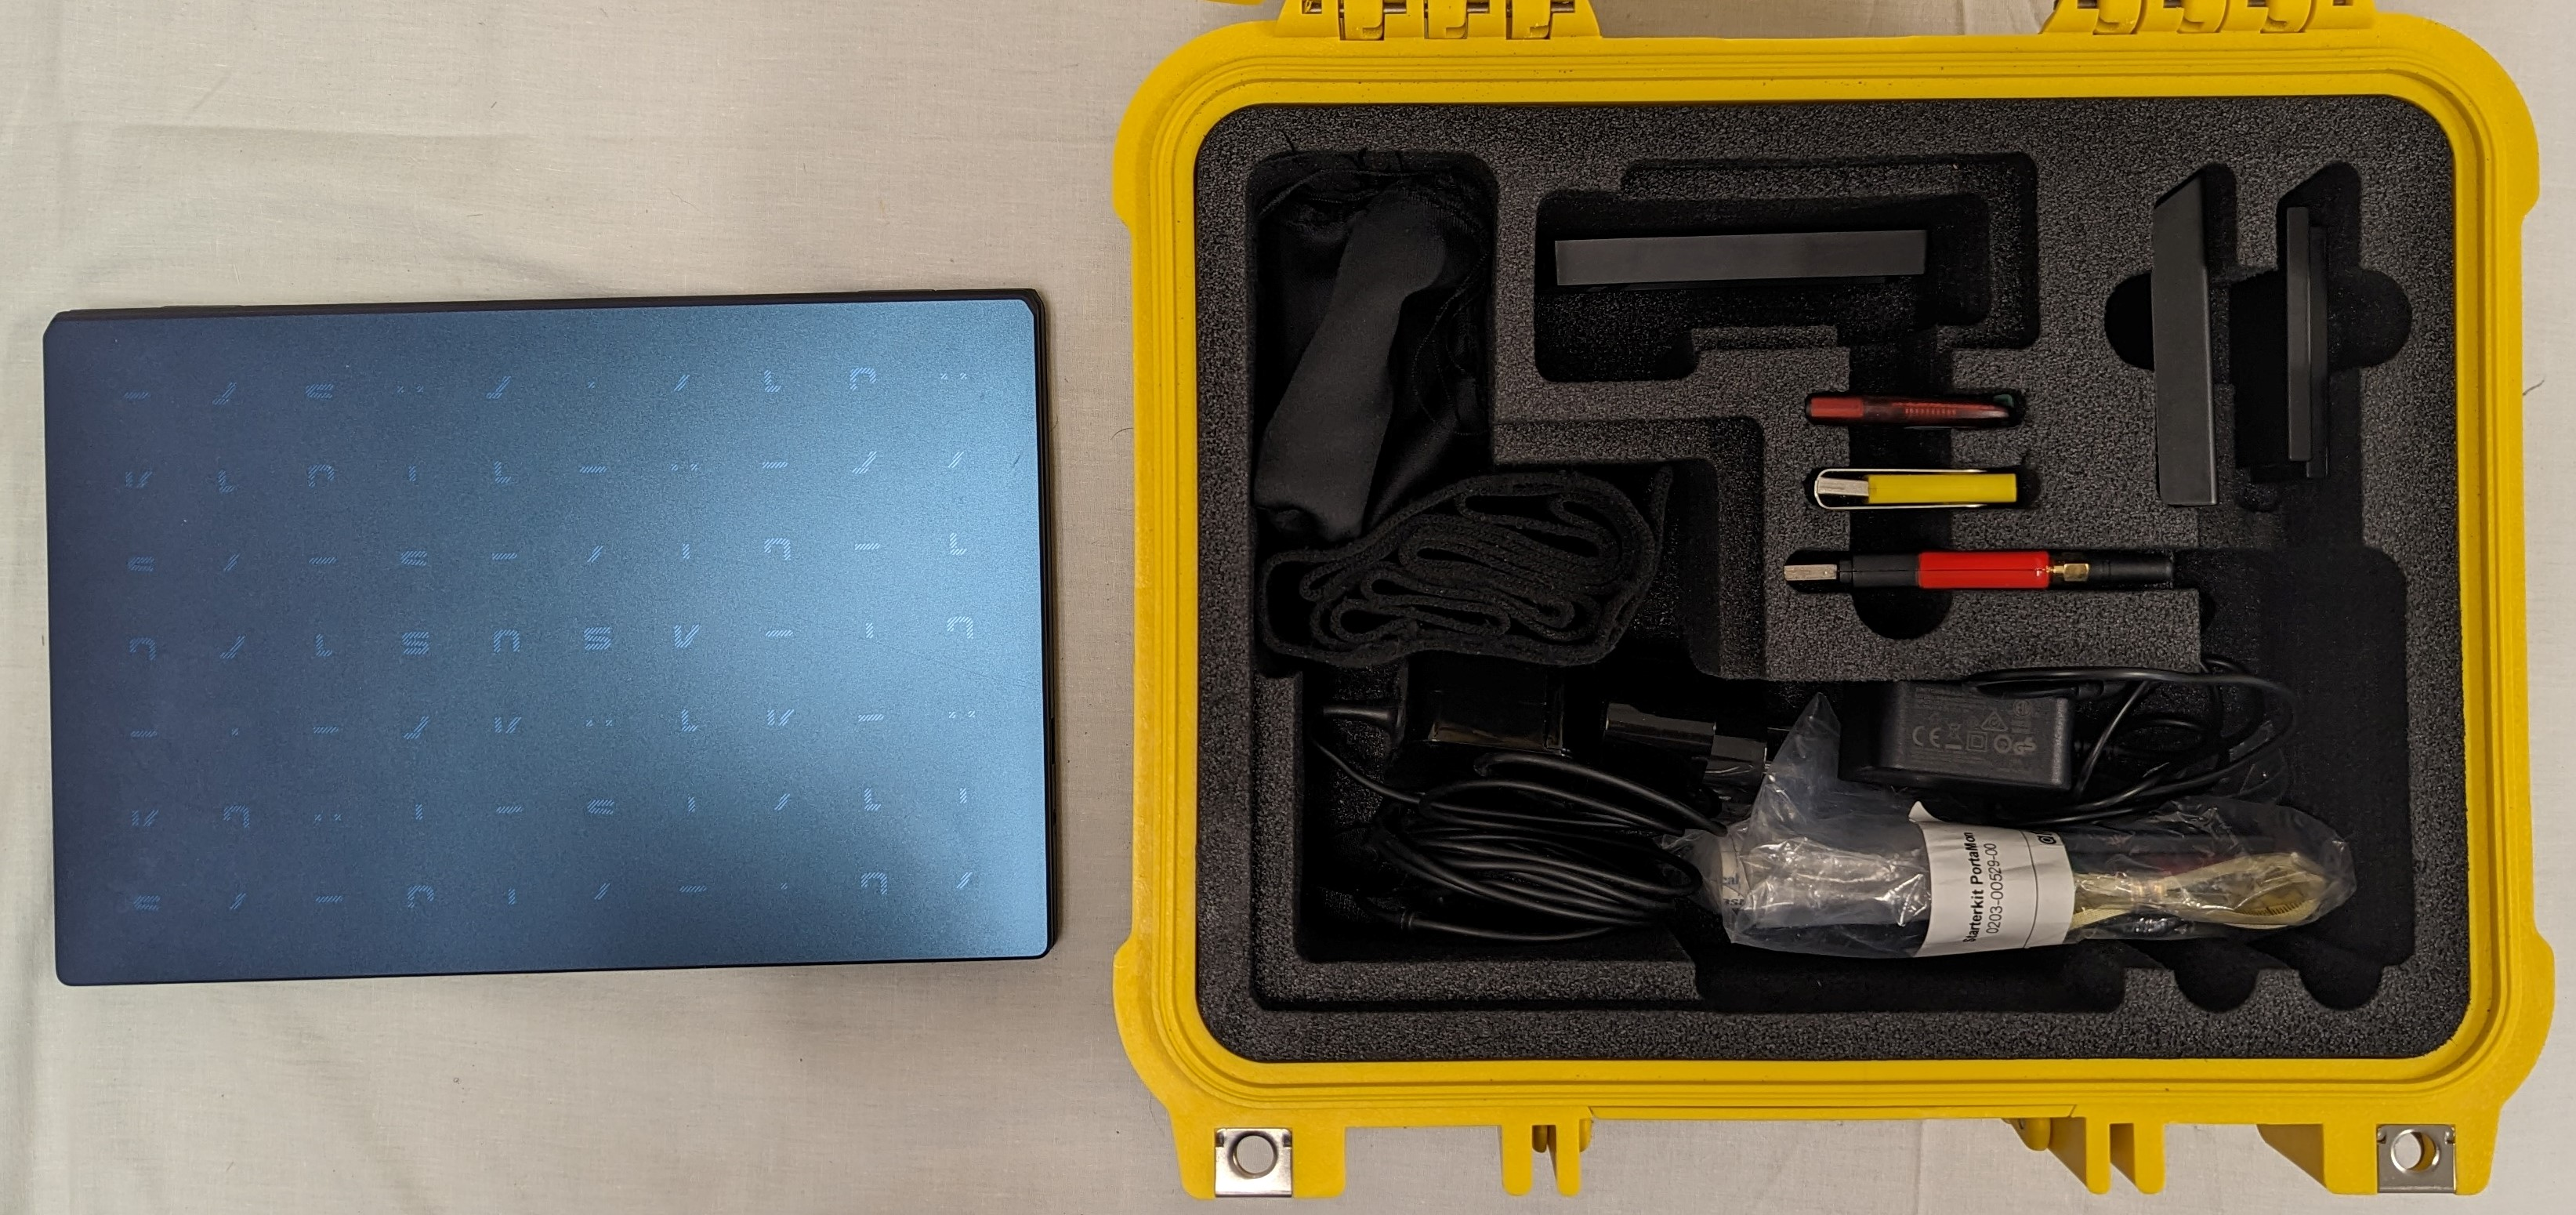
\includegraphics[width=1\linewidth]{images/portamon/portamoncase}

It contains the following:

\begin{itemize}
\tightlist
\item
  ASUS laptop
\item
  laptop charging chord with European to American outlet converter
\end{itemize}

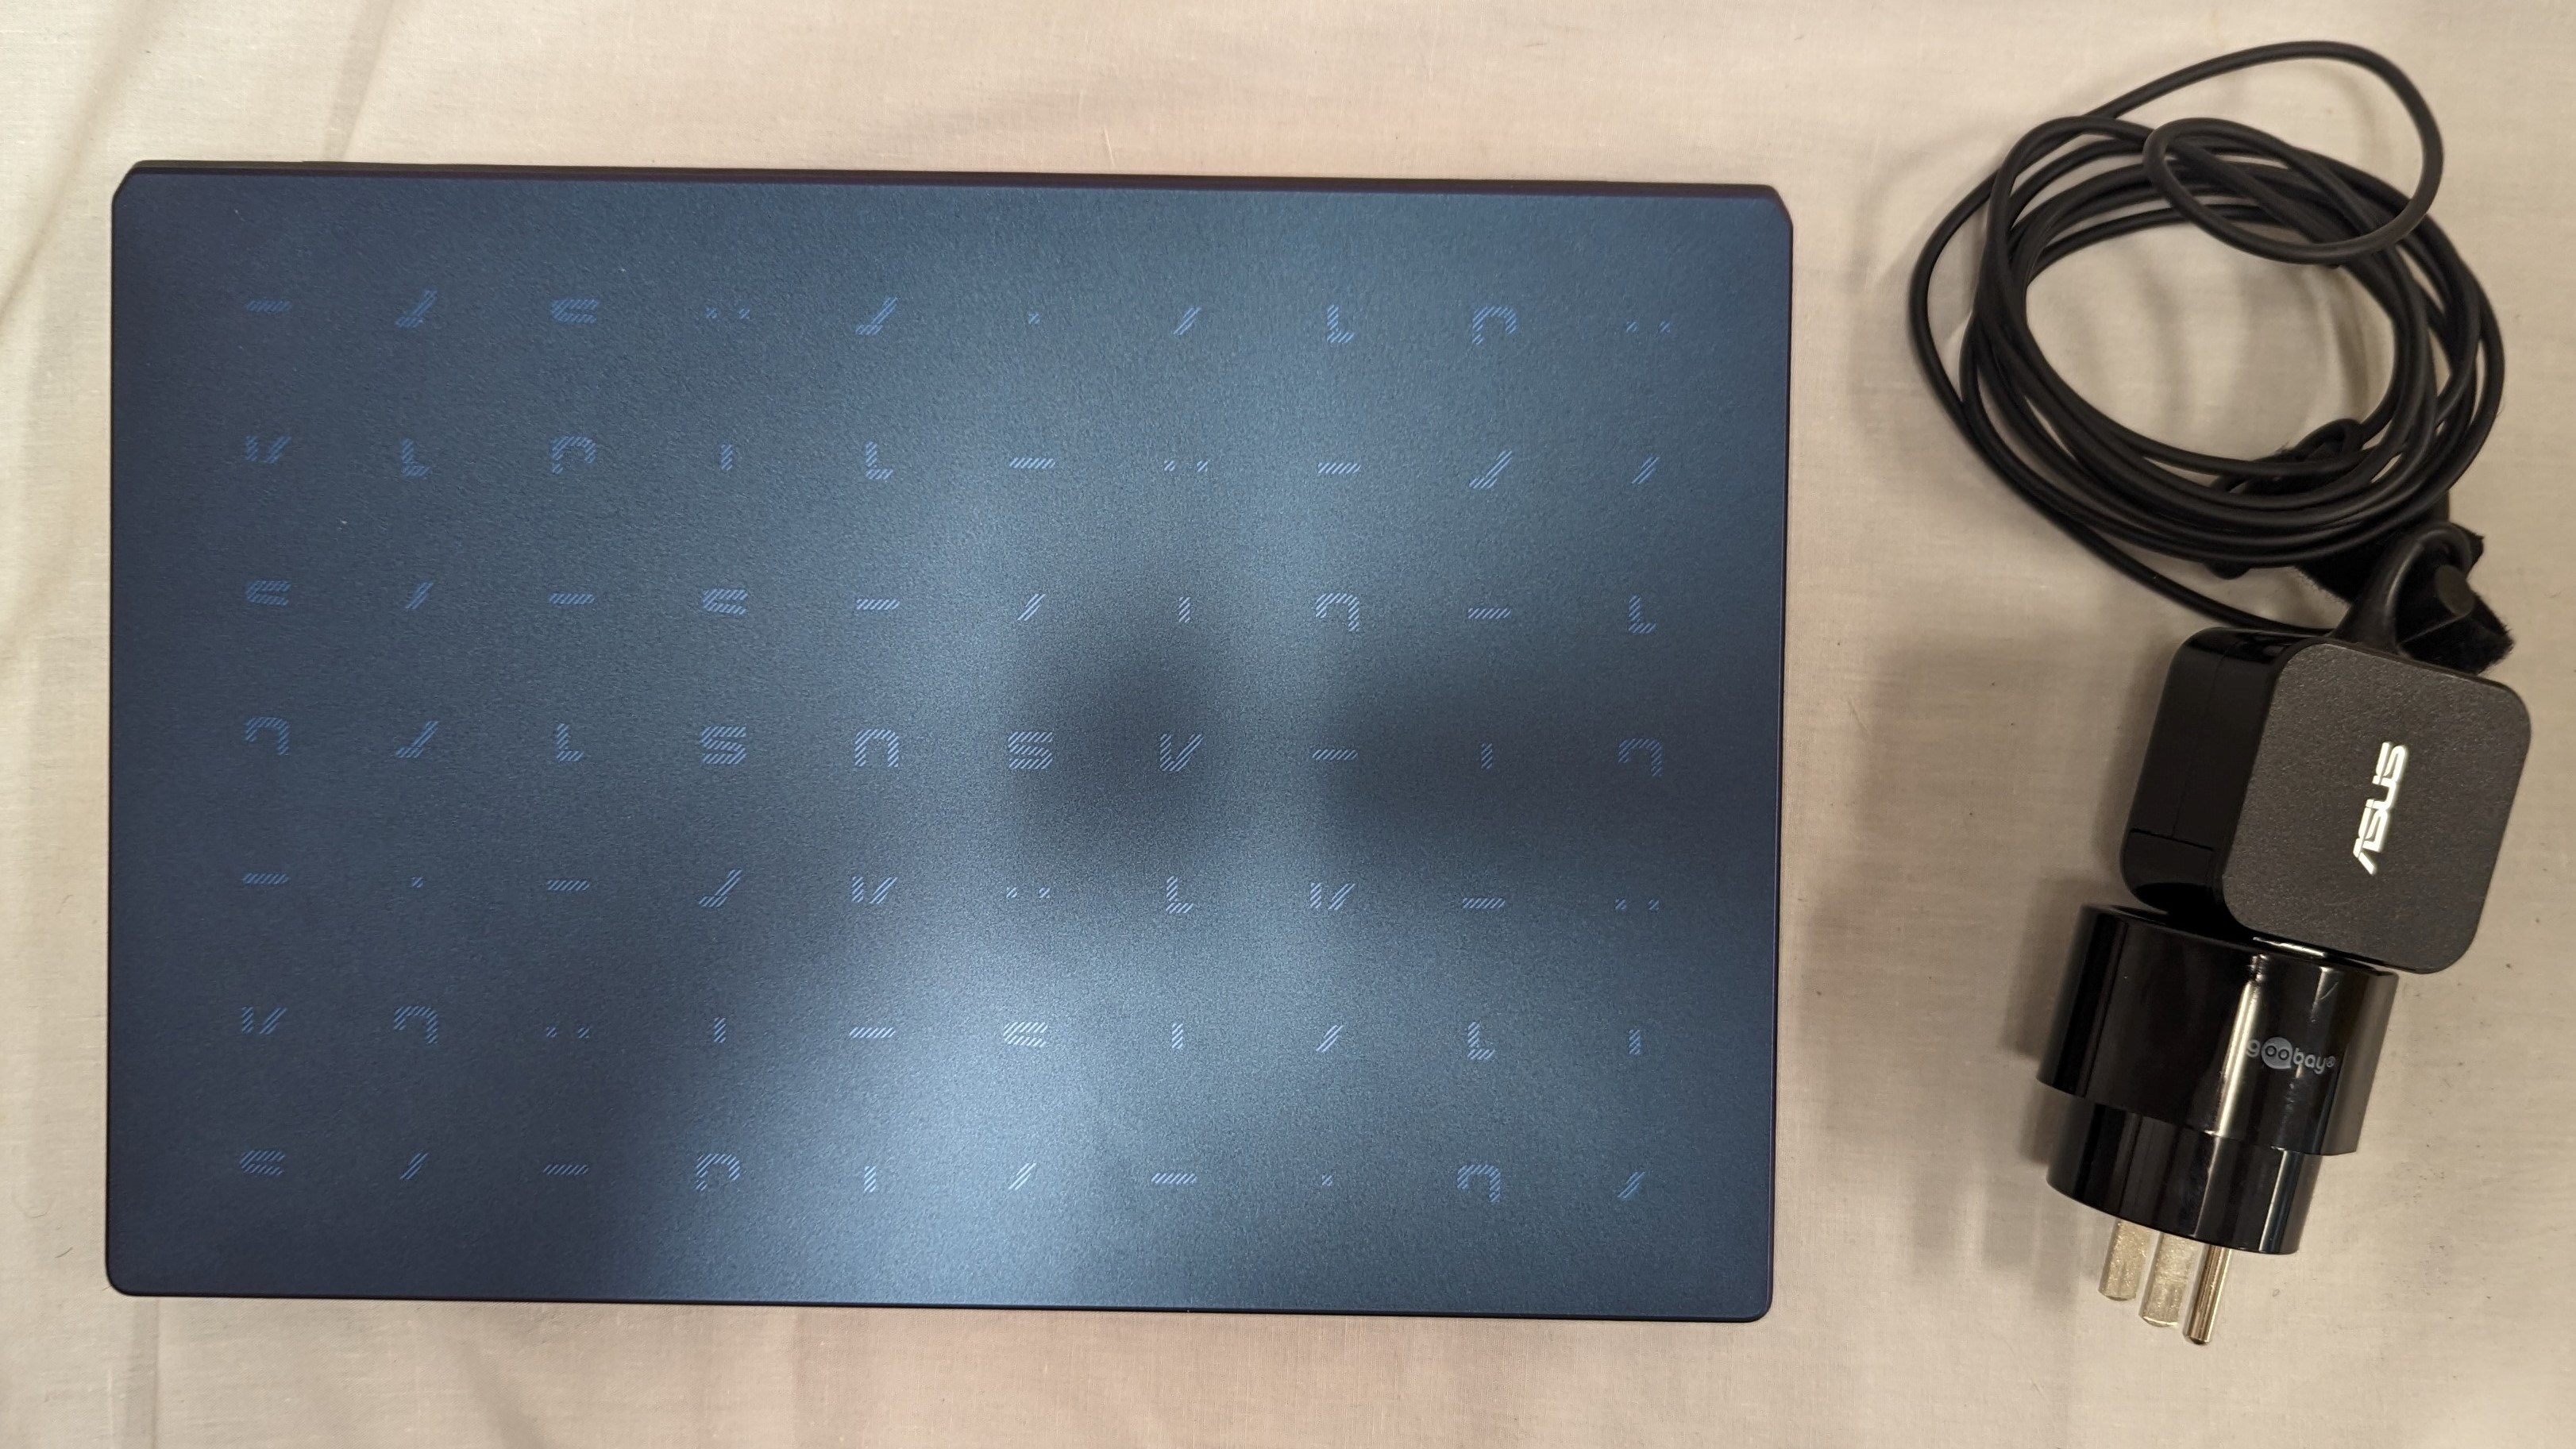
\includegraphics[width=1\linewidth]{images/portamon/asuslaptopandcharger}
- yellow Artinis Oxysoft USB
- Bluetooth dongle
- ROCKEY4ND license key

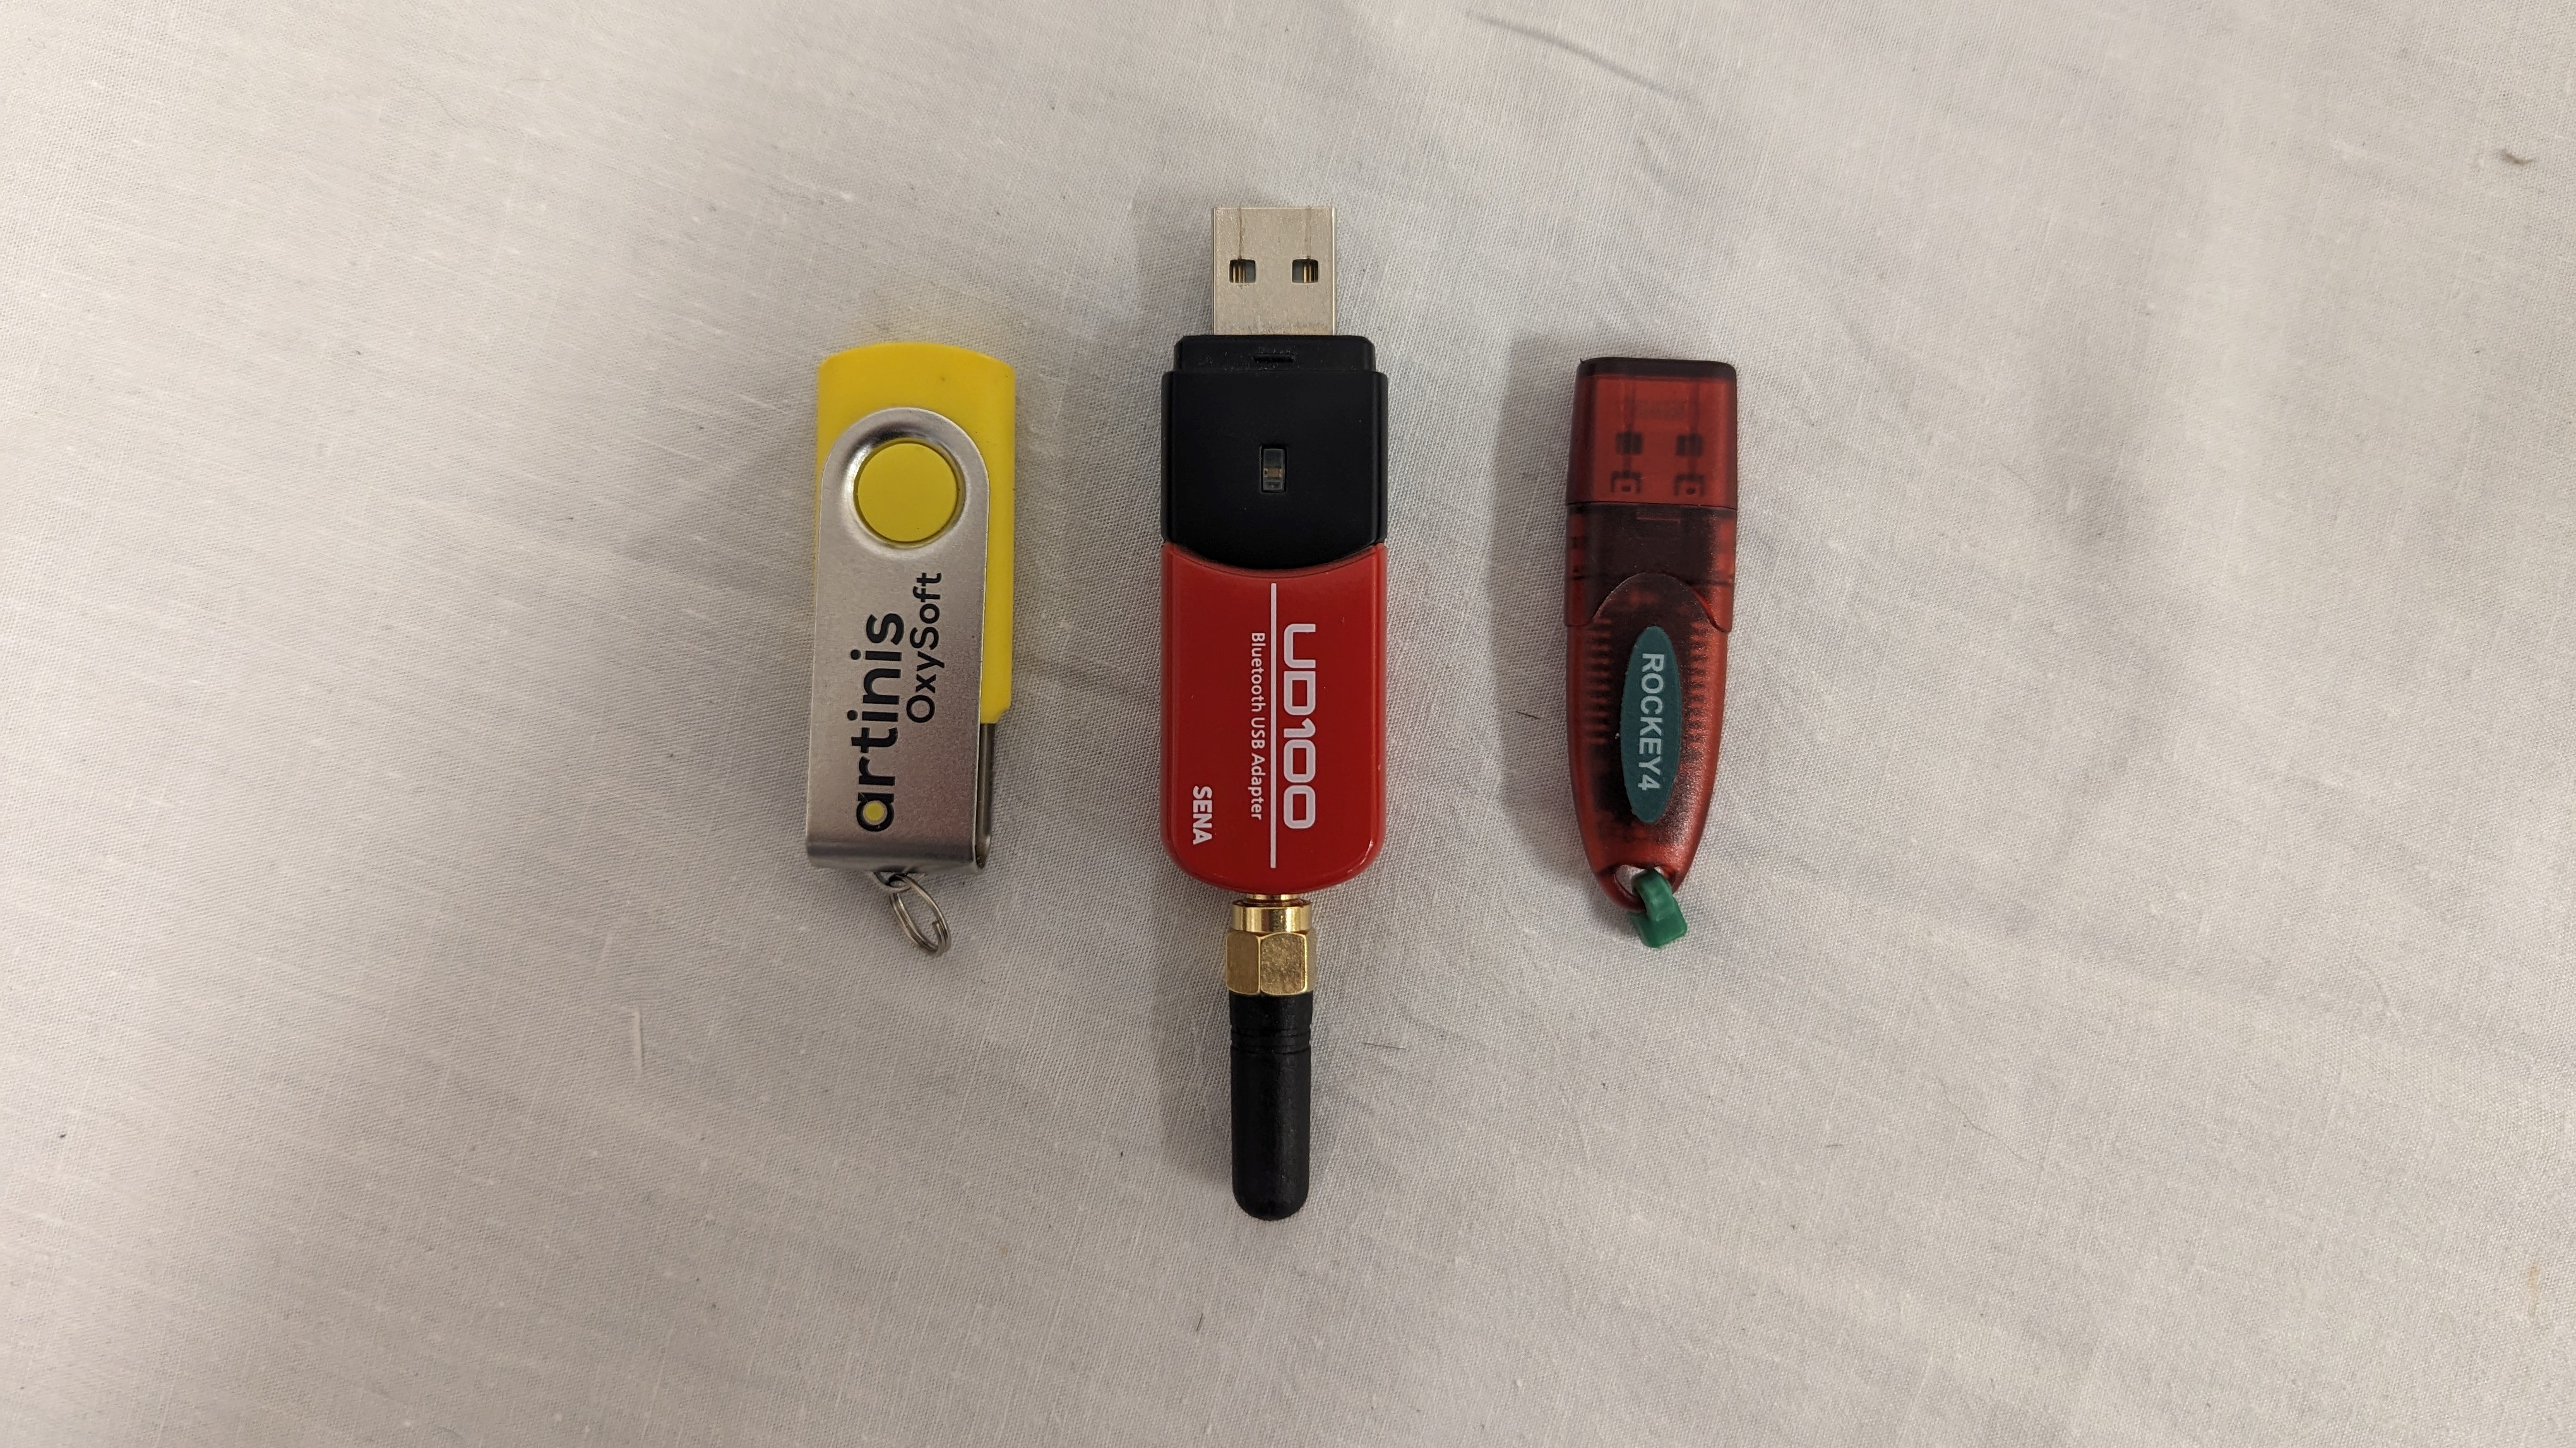
\includegraphics[width=1\linewidth]{images/portamon/laptopplugins}
- PortaMon device

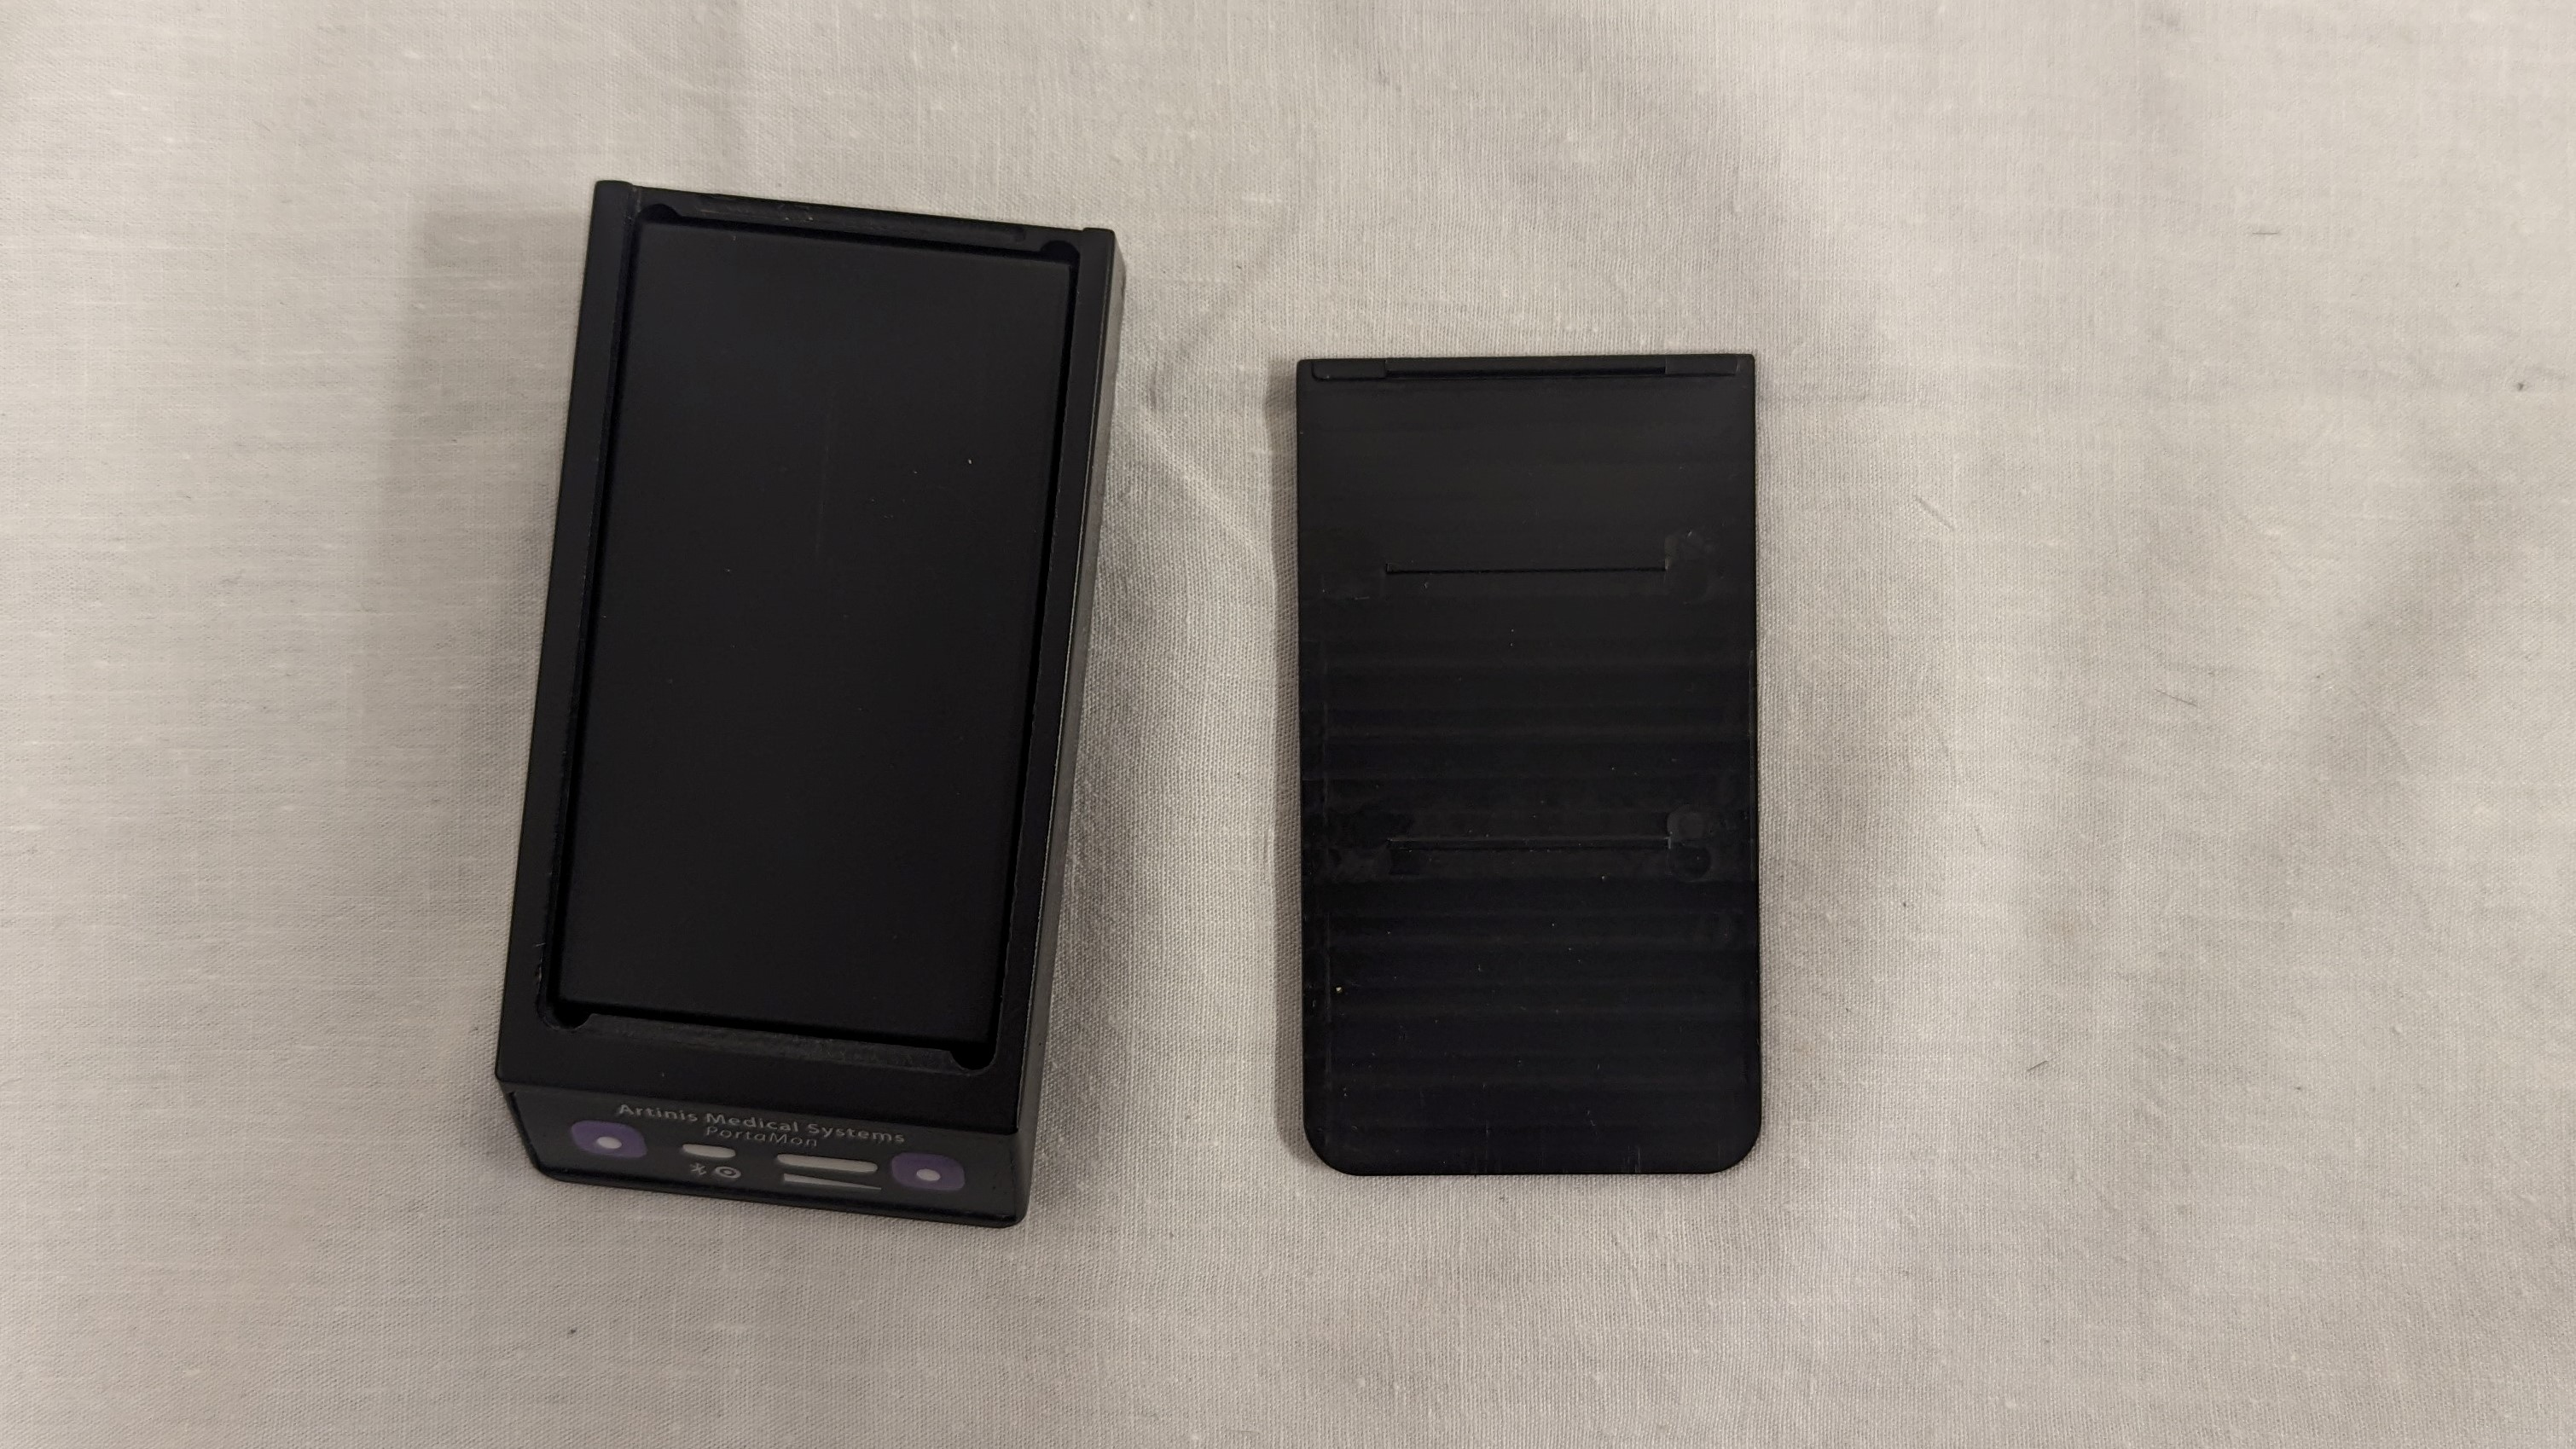
\includegraphics[width=1\linewidth]{images/portamon/portamonopen}
- two batteries
- battery charging dock
- micro-USB chord for battery charging dock

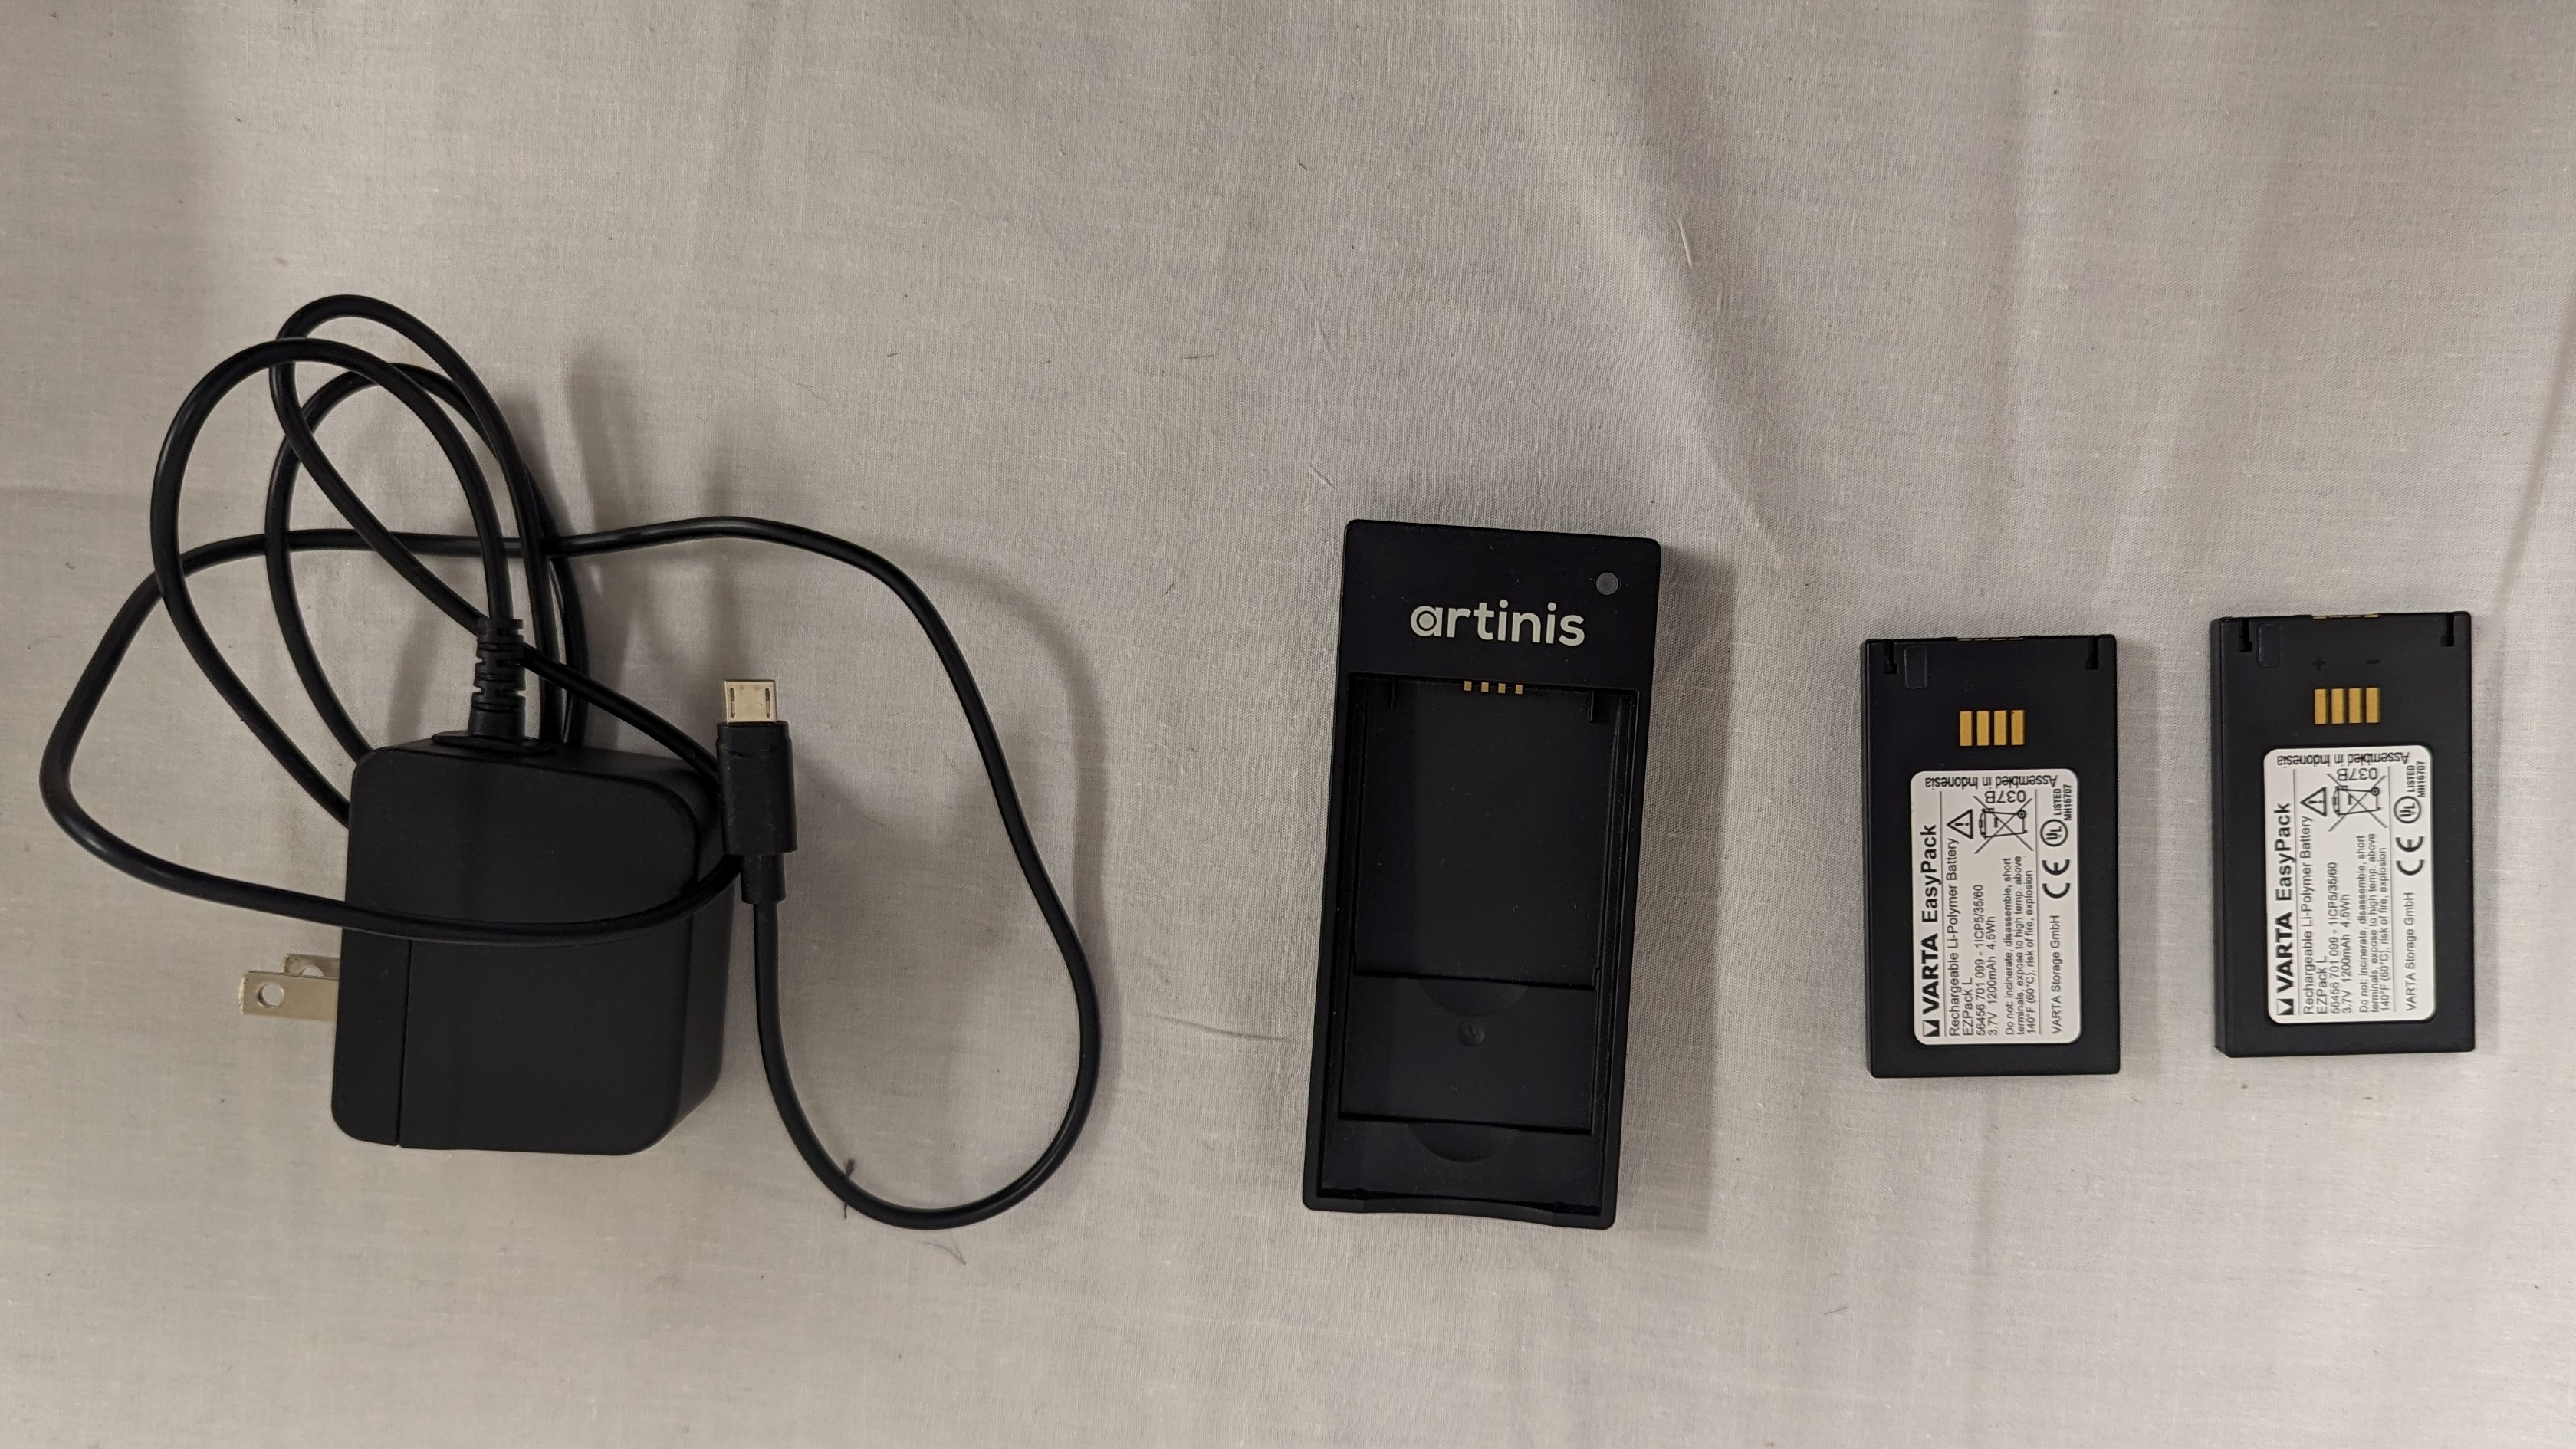
\includegraphics[width=1\linewidth]{images/portamon/portamonbatteriesandcharger}

\hypertarget{Oxysoft}{%
\section{Oysoft}\label{Oxysoft}}

Oxysoft is the software created by Artinis Medical Systems to connect with the PortaMon, collect, and analyze data.

Oxysoft is installed on the ASUS laptops that go with the yellow cases. These laptops do not have any PrismaHealth or USC SoMG software on them. If someone should want to install Oxysoft on a PrismaHealth or USC SoMG computer, Oxysoft will have to be approved by the respective organization's IT team.

Oxysoft has been approved to be on Sara Biddle's PrismaHealth desktop computer by PrismaHealth's IT. No other PrismaHealth or USC SoMG computers have Oxysoft installed.

If you wish to install Oxysoft on a personal computer or have been approved to install Oxysoft on an organization's computer, plug the yellow Artinis Oxysoft USB into the computer and run the installer.

\begin{itemize}
\item
  Oxysoft uses a legacy Bluetooth dongle to connect to the PortaMon. This makes using Oxysoft on a computer with the most up to date Windows difficult. It is easier to collect data on the ASUS laptops, which are default configured to use the Bluetooth dongle, and then export the data for analysis.
\item
  Oxysoft creates files with the extension \texttt{.oxy4} for every new measurement.
\end{itemize}

\hypertarget{PortaMon-Batteries}{%
\section{Batteries}\label{PortaMon-Batteries}}

The PortaMon batteries can hold up to 8 hours of power for the device. Make sure they are fully charged prior to a patient's visit.

Plug the micro-USB into the battery charging dock. Plug this into an outlet. Place the battery into the dock, sticker side down. The three metal connectors on the narrow side of the battery must be touching the three metal connectors on the charging dock. If the battery is correctly placed in the dock, an LED will light up. When the battery is fully charged, the LED will be green.

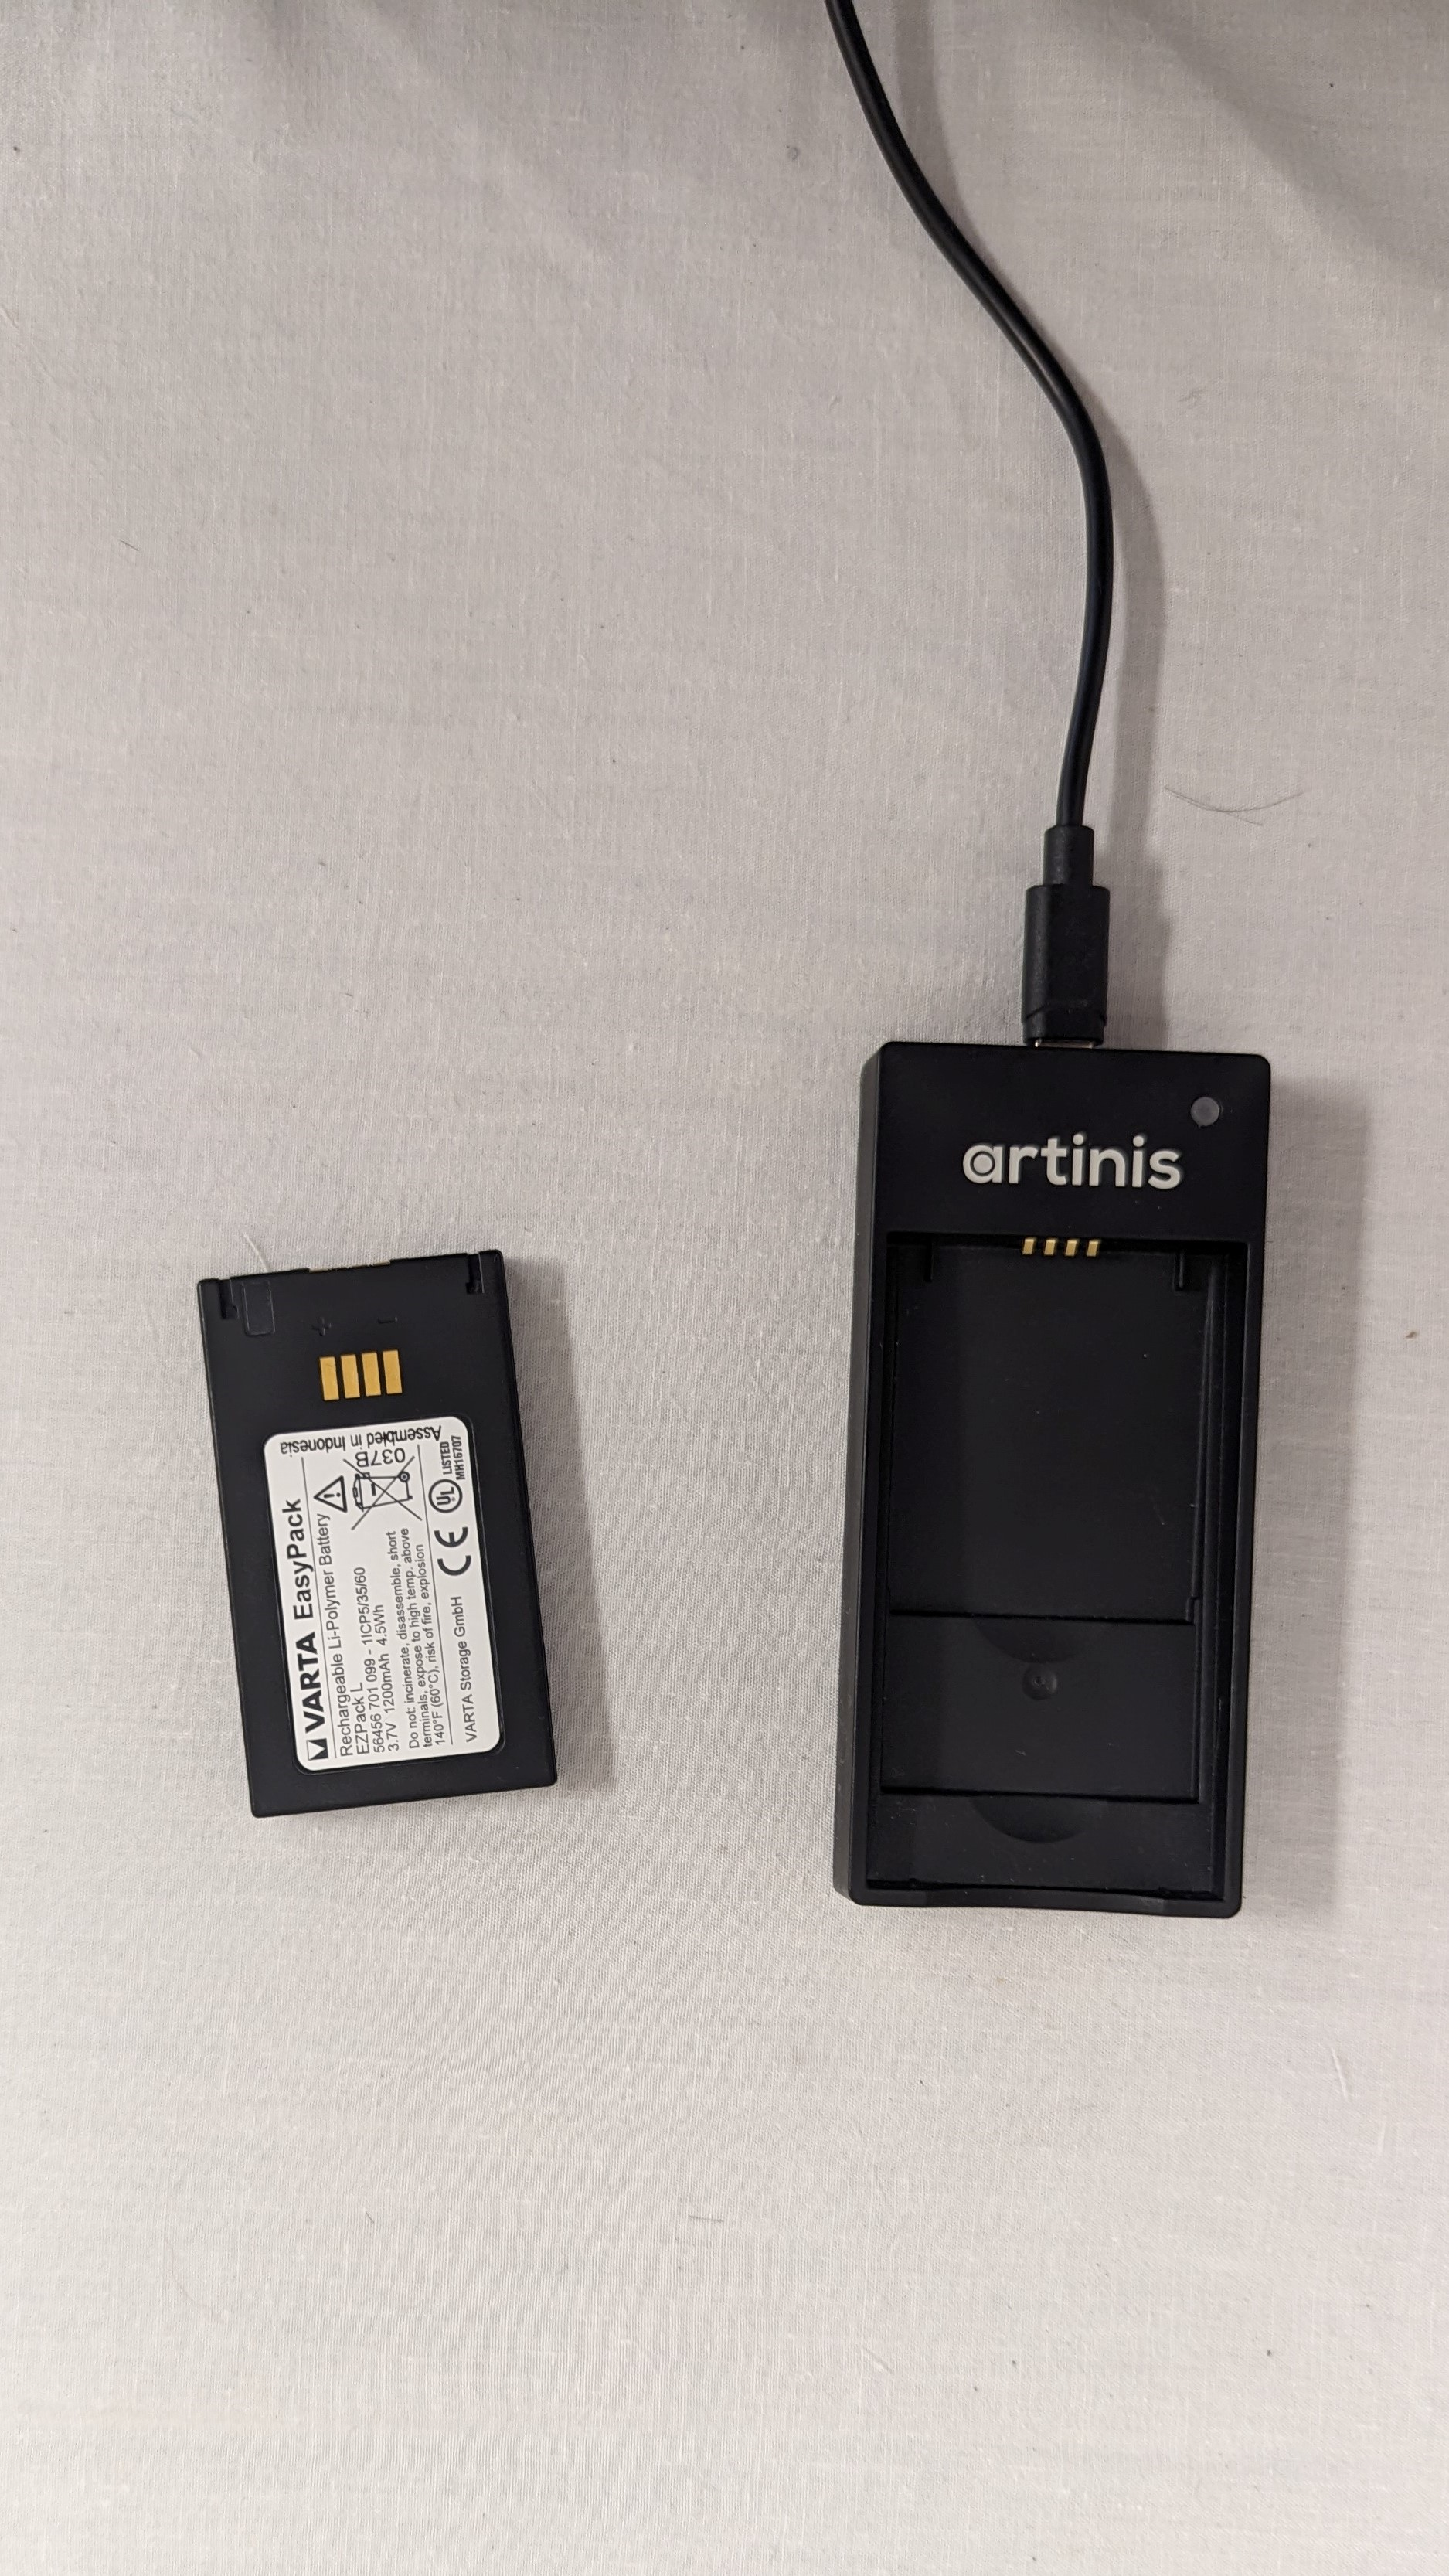
\includegraphics[width=0.33\linewidth]{images/portamon/portamonbatteryandchargerplug}
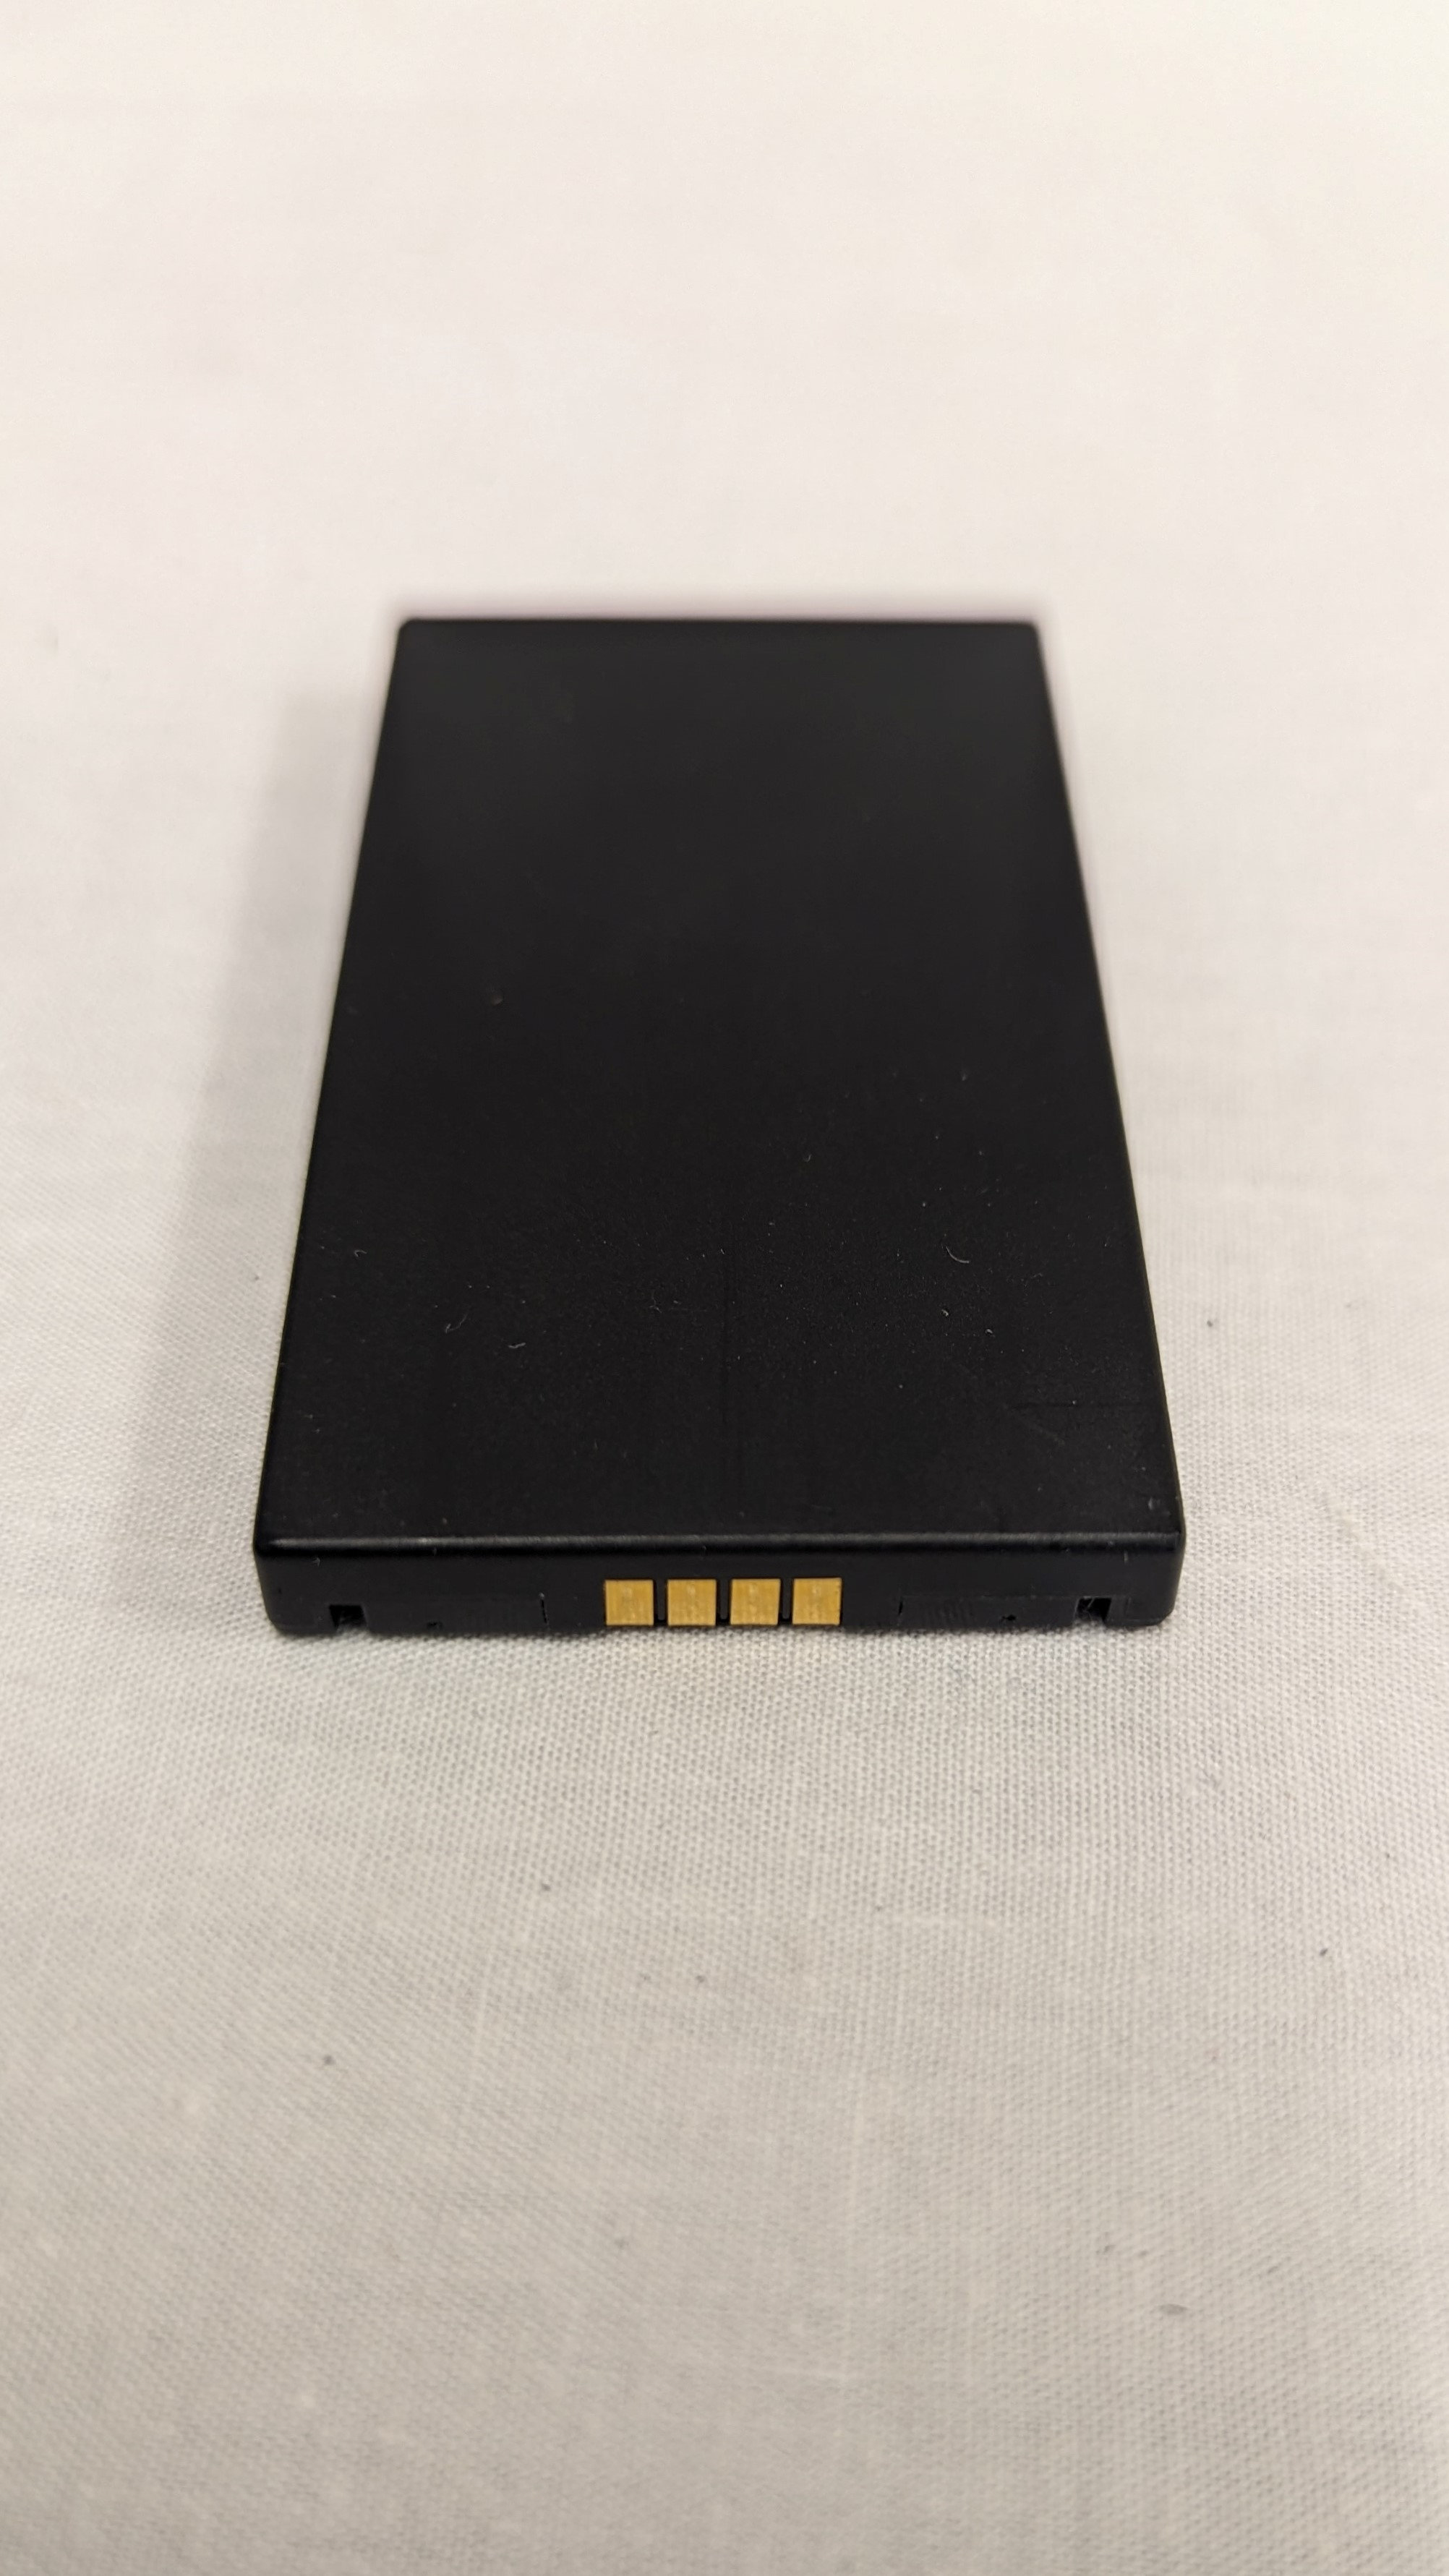
\includegraphics[width=0.33\linewidth]{images/portamon/portamonbatterychargingport}
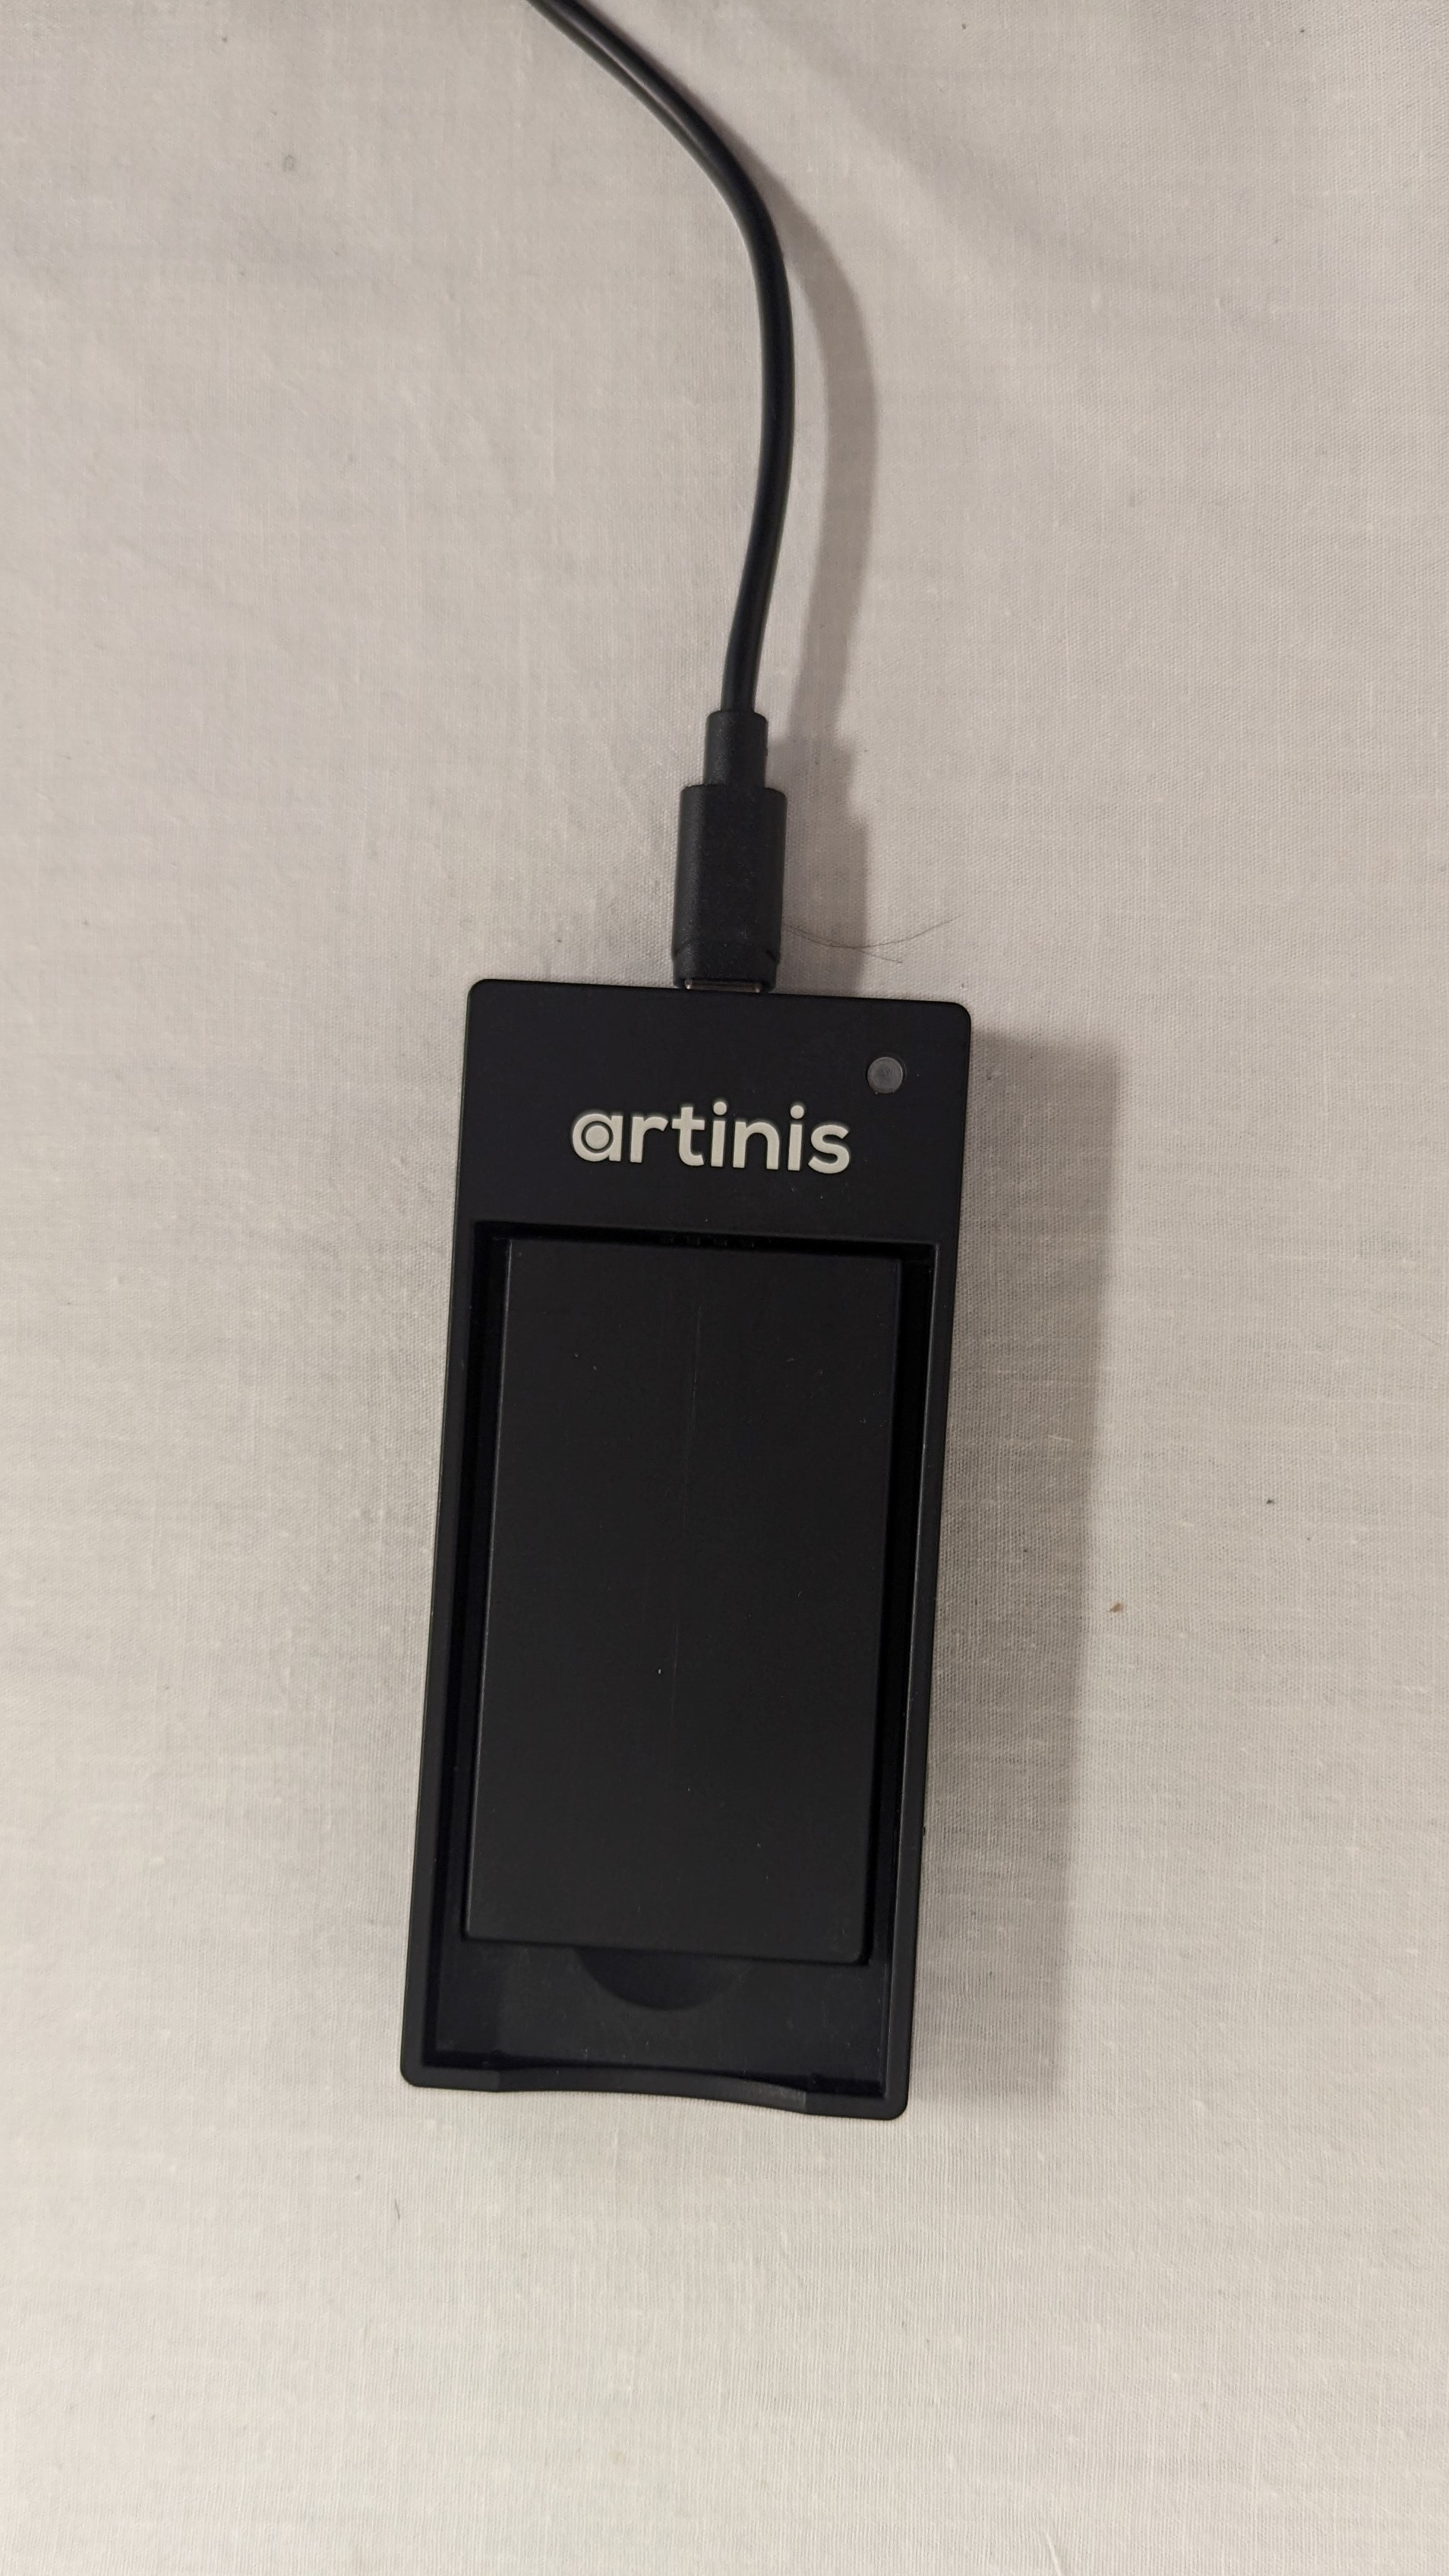
\includegraphics[width=0.33\linewidth]{images/portamon/portamonbatteryincharger}

\hypertarget{PortaMon-BeforeDataCollection}{%
\section{Before Data Collection}\label{PortaMon-BeforeDataCollection}}

\hypertarget{PortaMon-Prep}{%
\subsection{Instrument Preparation for Data Collection}\label{PortaMon-Prep}}

\begin{itemize}
\tightlist
\item
  Place a fully charged battery in the PortaMon, with the three connectors on the battery touching the three connectors in the PortaMon.
\item
  Slide the top of the PortaMon back in until it clicks into place. If the battery is charged and placed correctly, LEDs on the bottom of the PortaMon will light up.
\end{itemize}

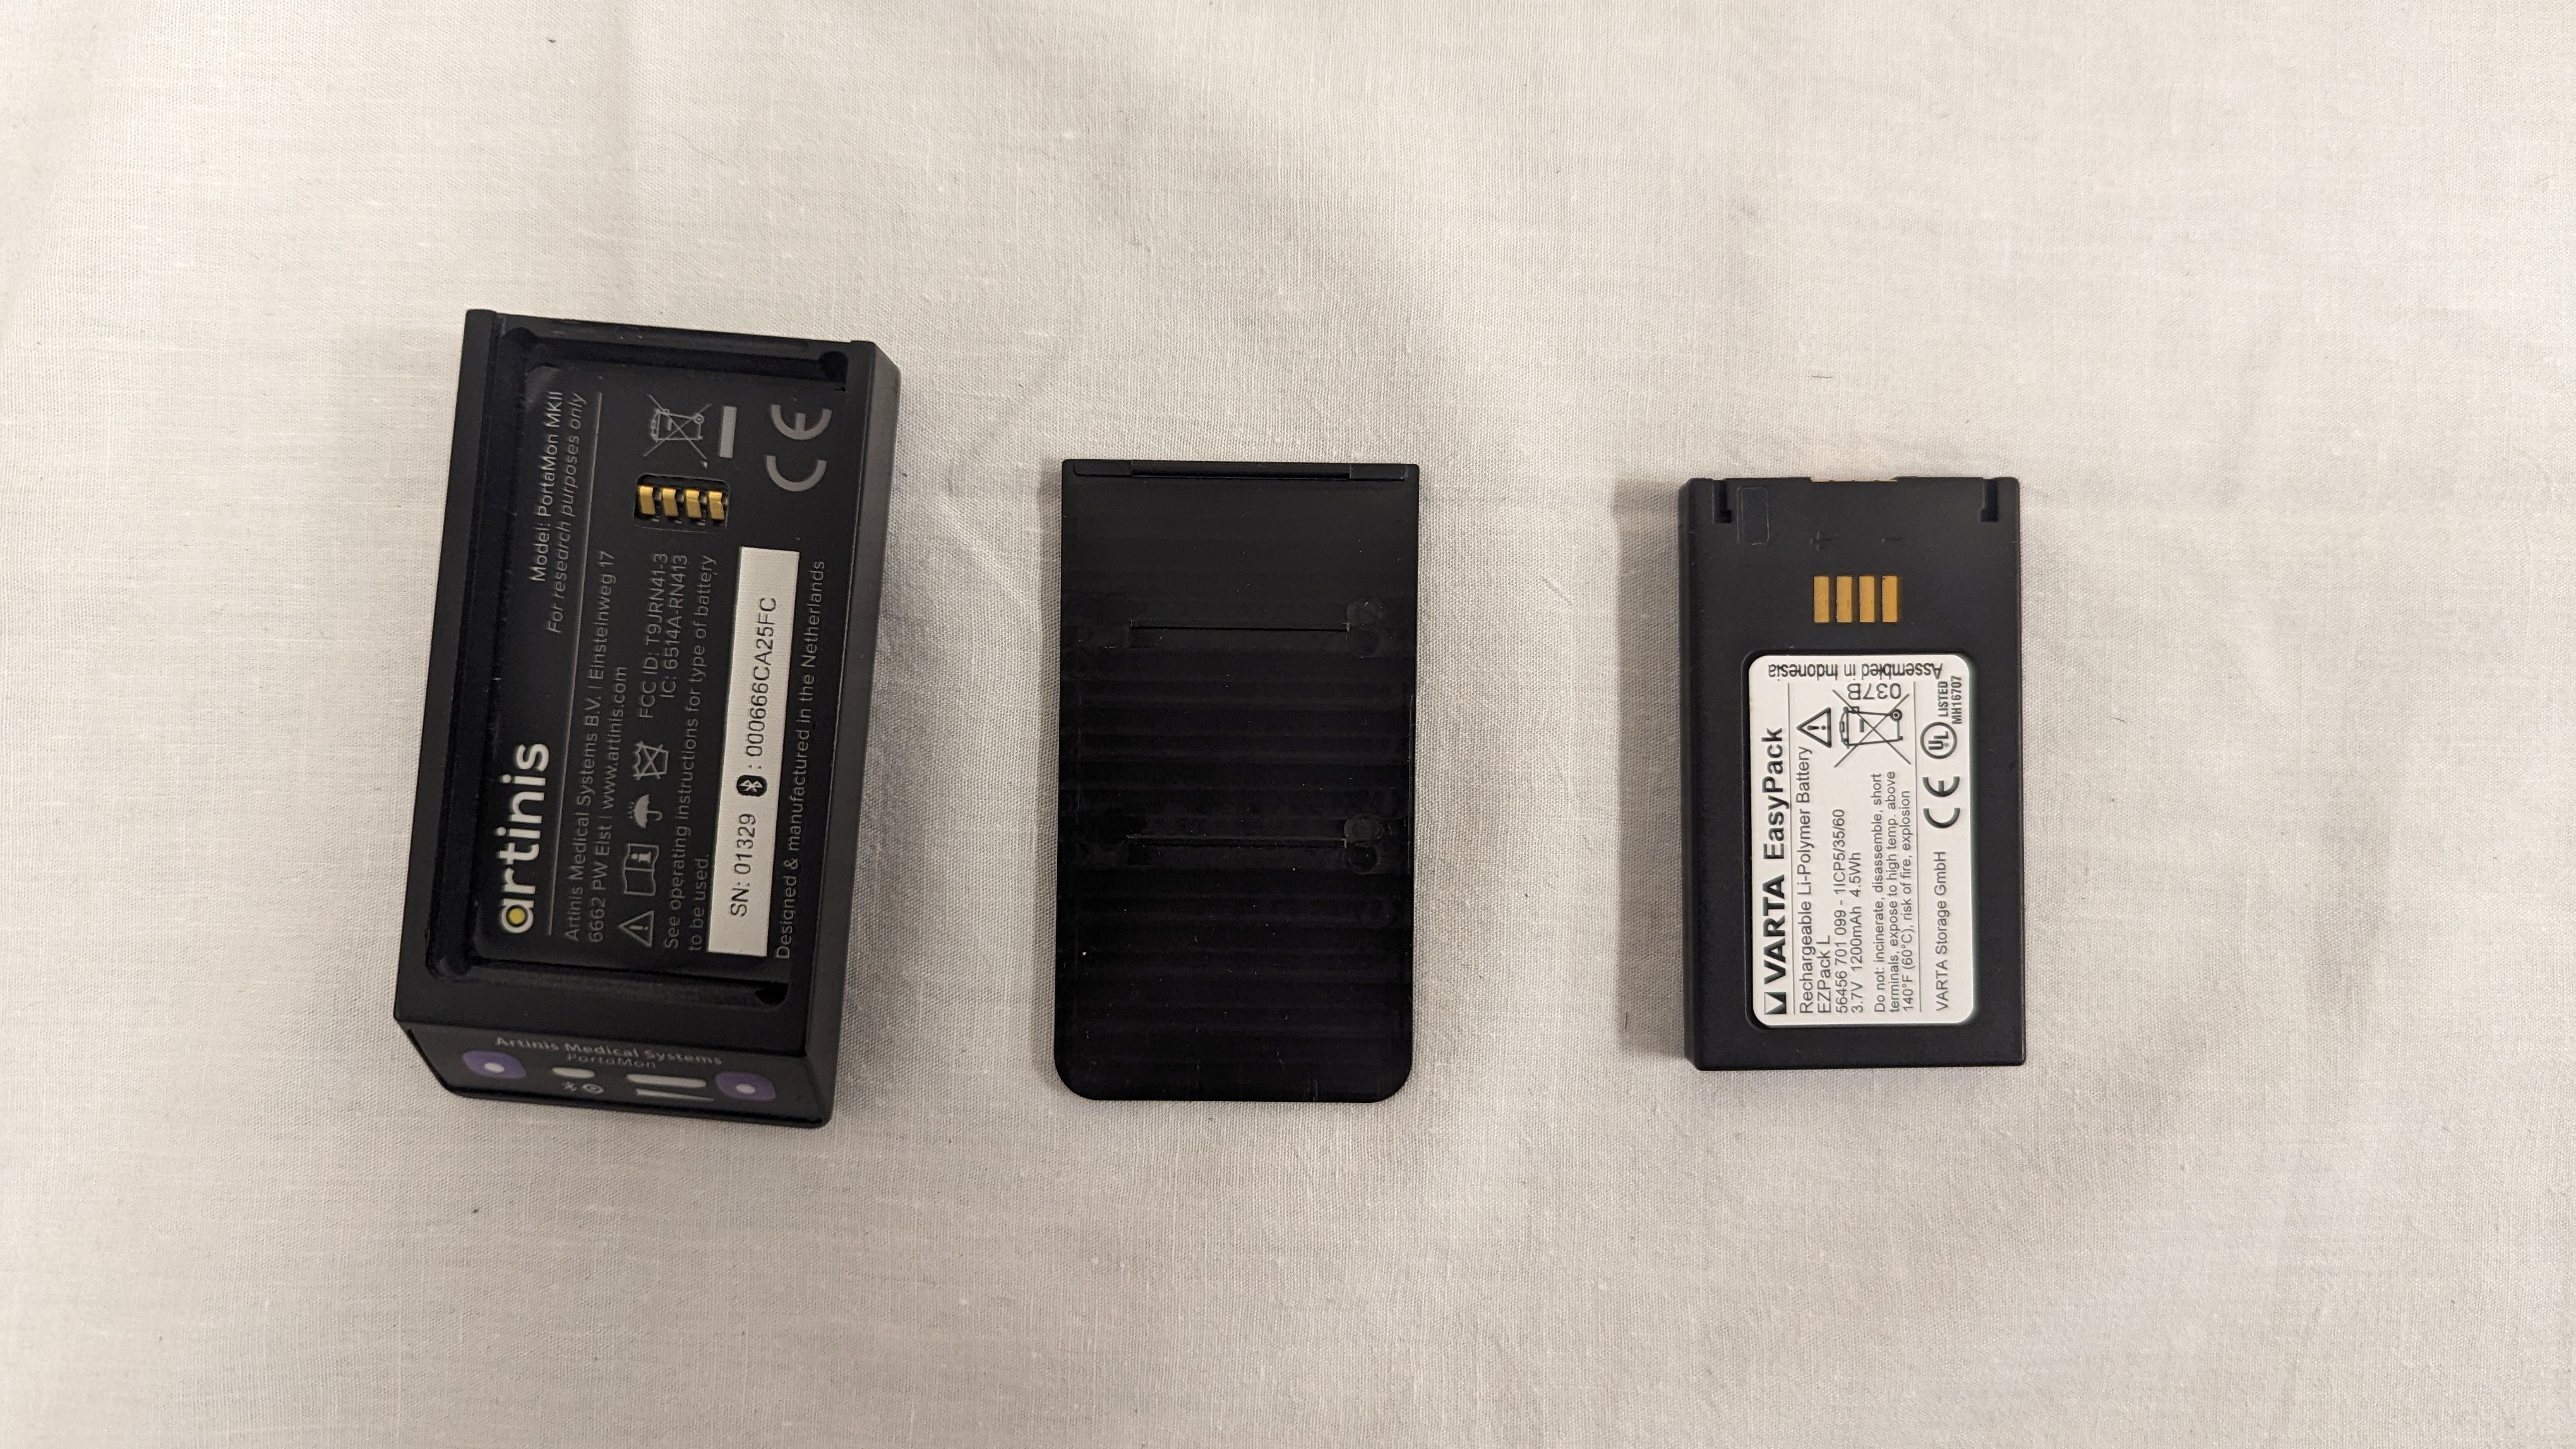
\includegraphics[width=0.5\linewidth]{images/portamon/portamonandbattery}
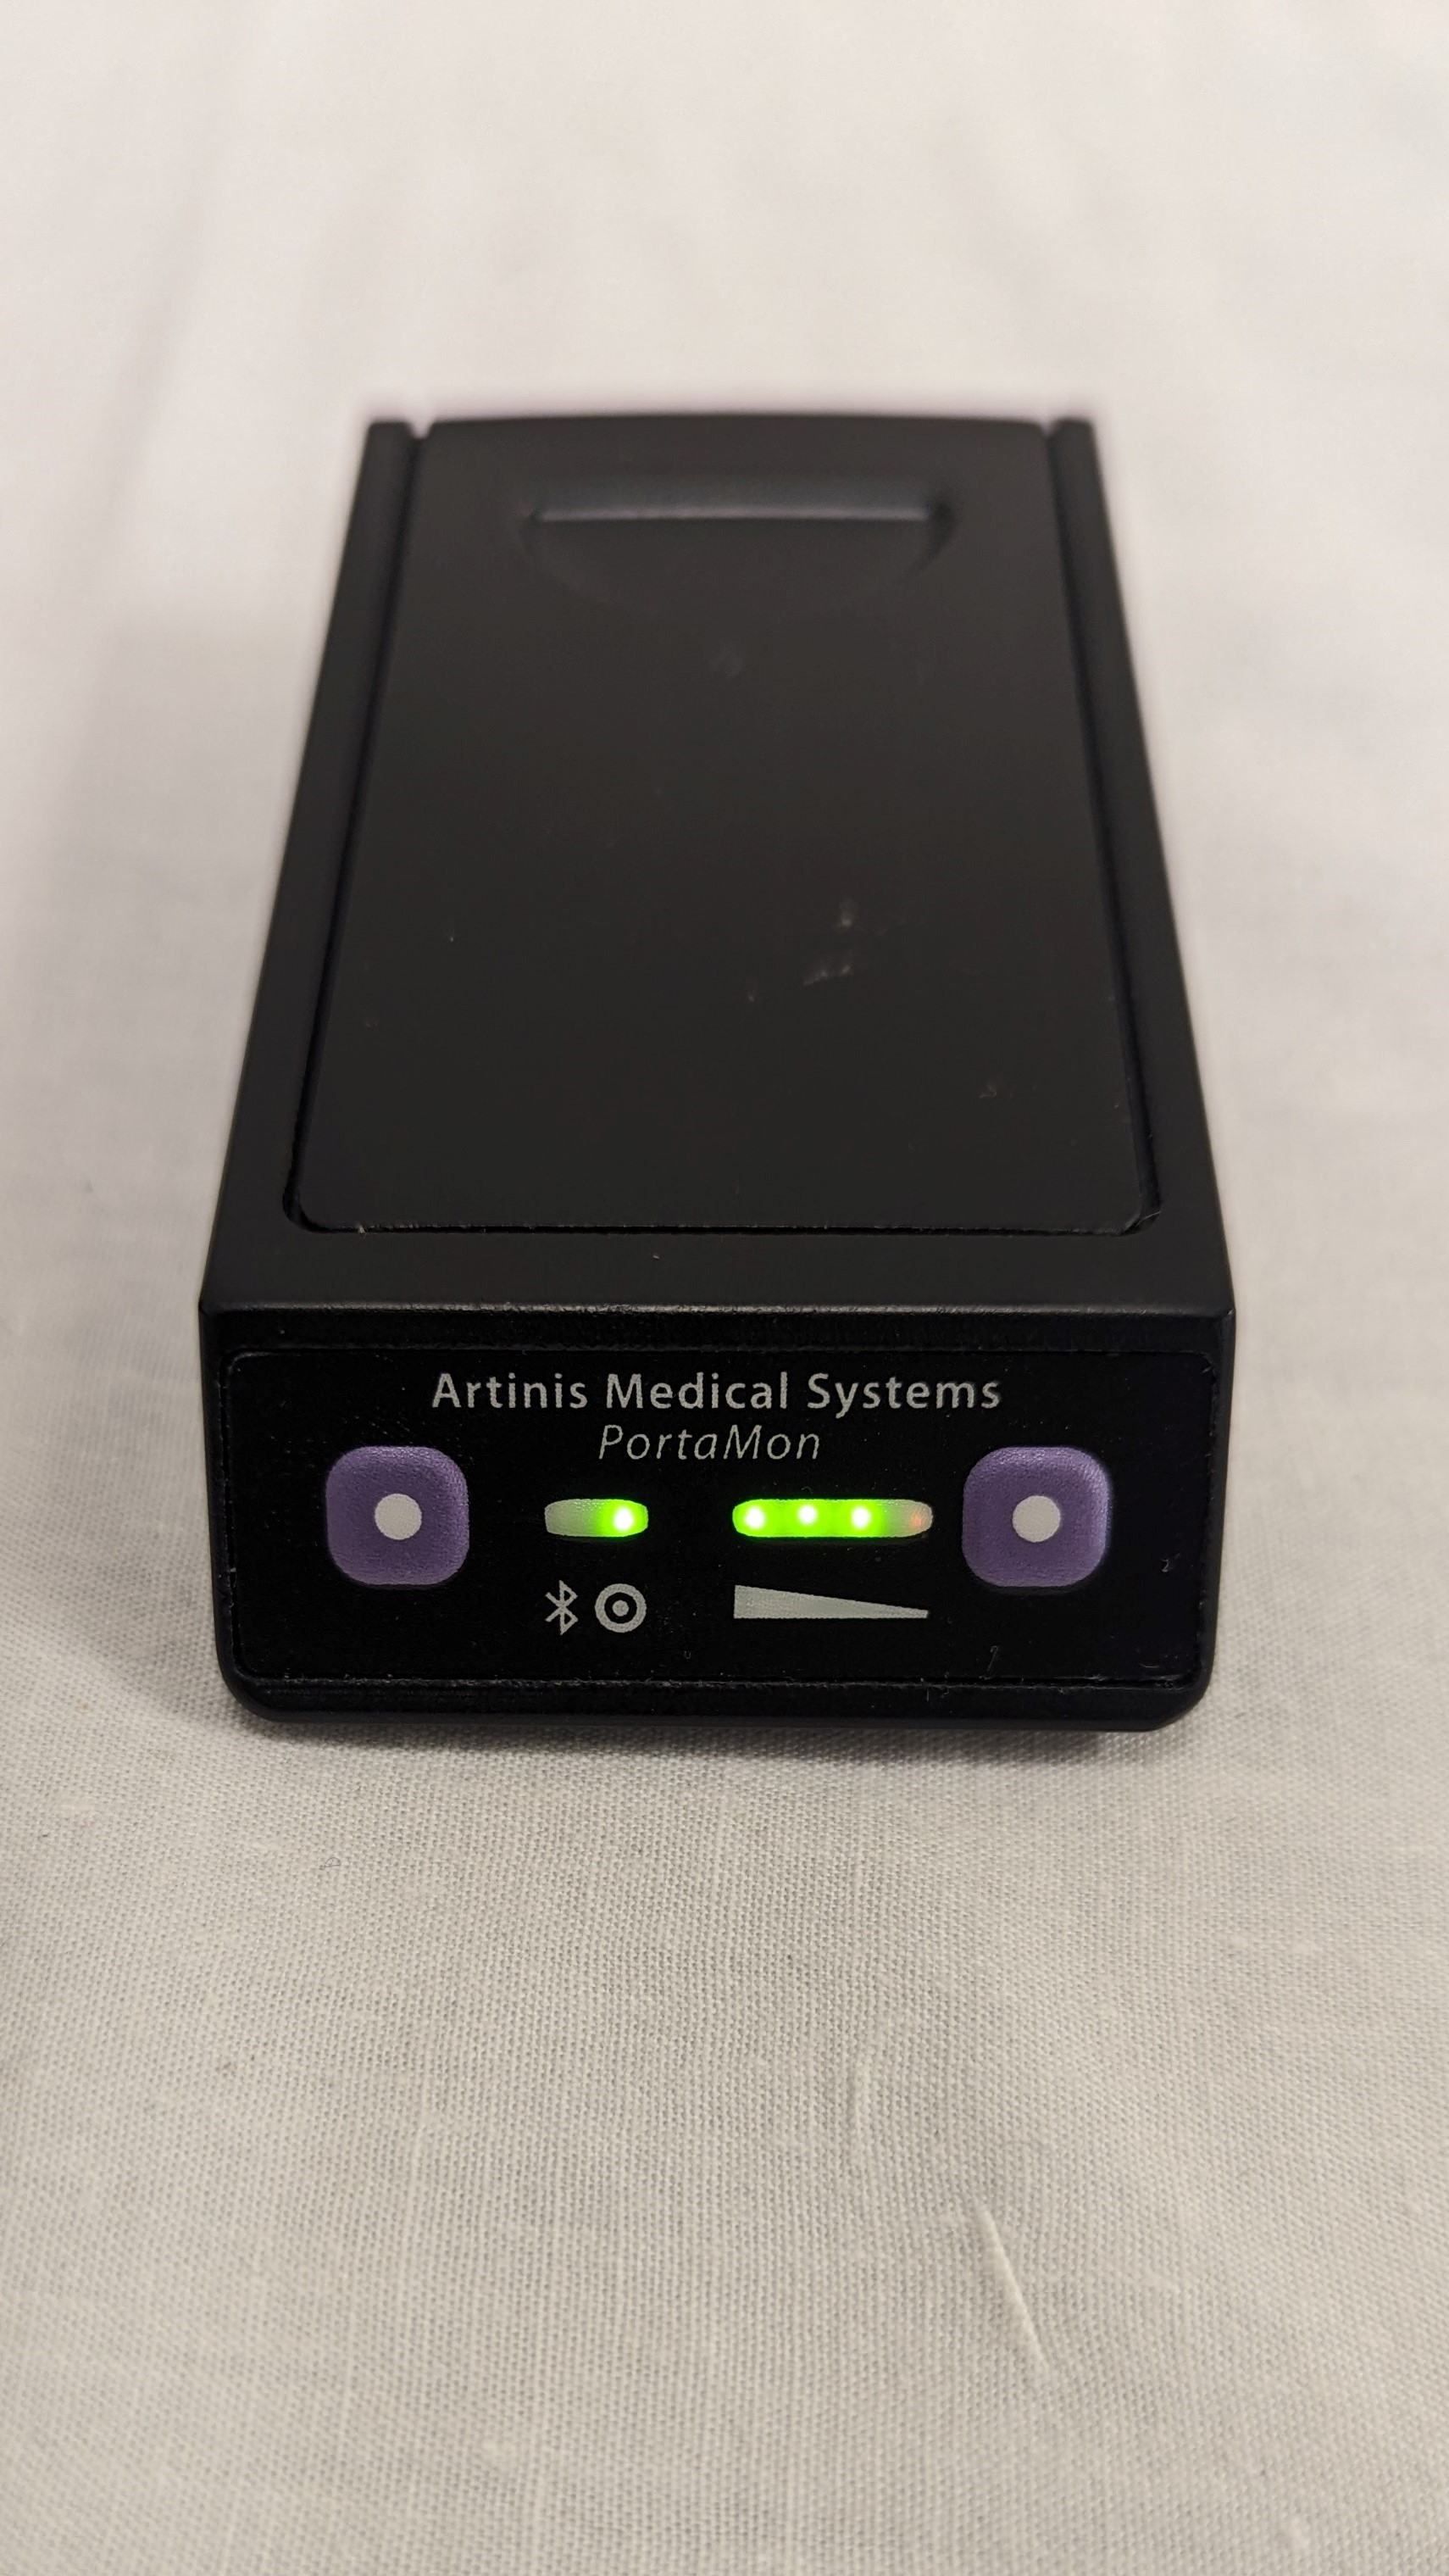
\includegraphics[width=0.5\linewidth]{images/portamon/portamonon}

\begin{itemize}
\tightlist
\item
  Wrap the PortaMon in clear saran wrap and tape the saran wrap in place. This prevents sweat and other moisture from getting in to the PortaMon. Since the PortaMon has electronic parts, it cannot be sterilized using liquids and the saran wrap means we do not have to sterilize the device itself. When testing is complete, pull saran wrap and tape off the PortaMon and throw it away.
\end{itemize}

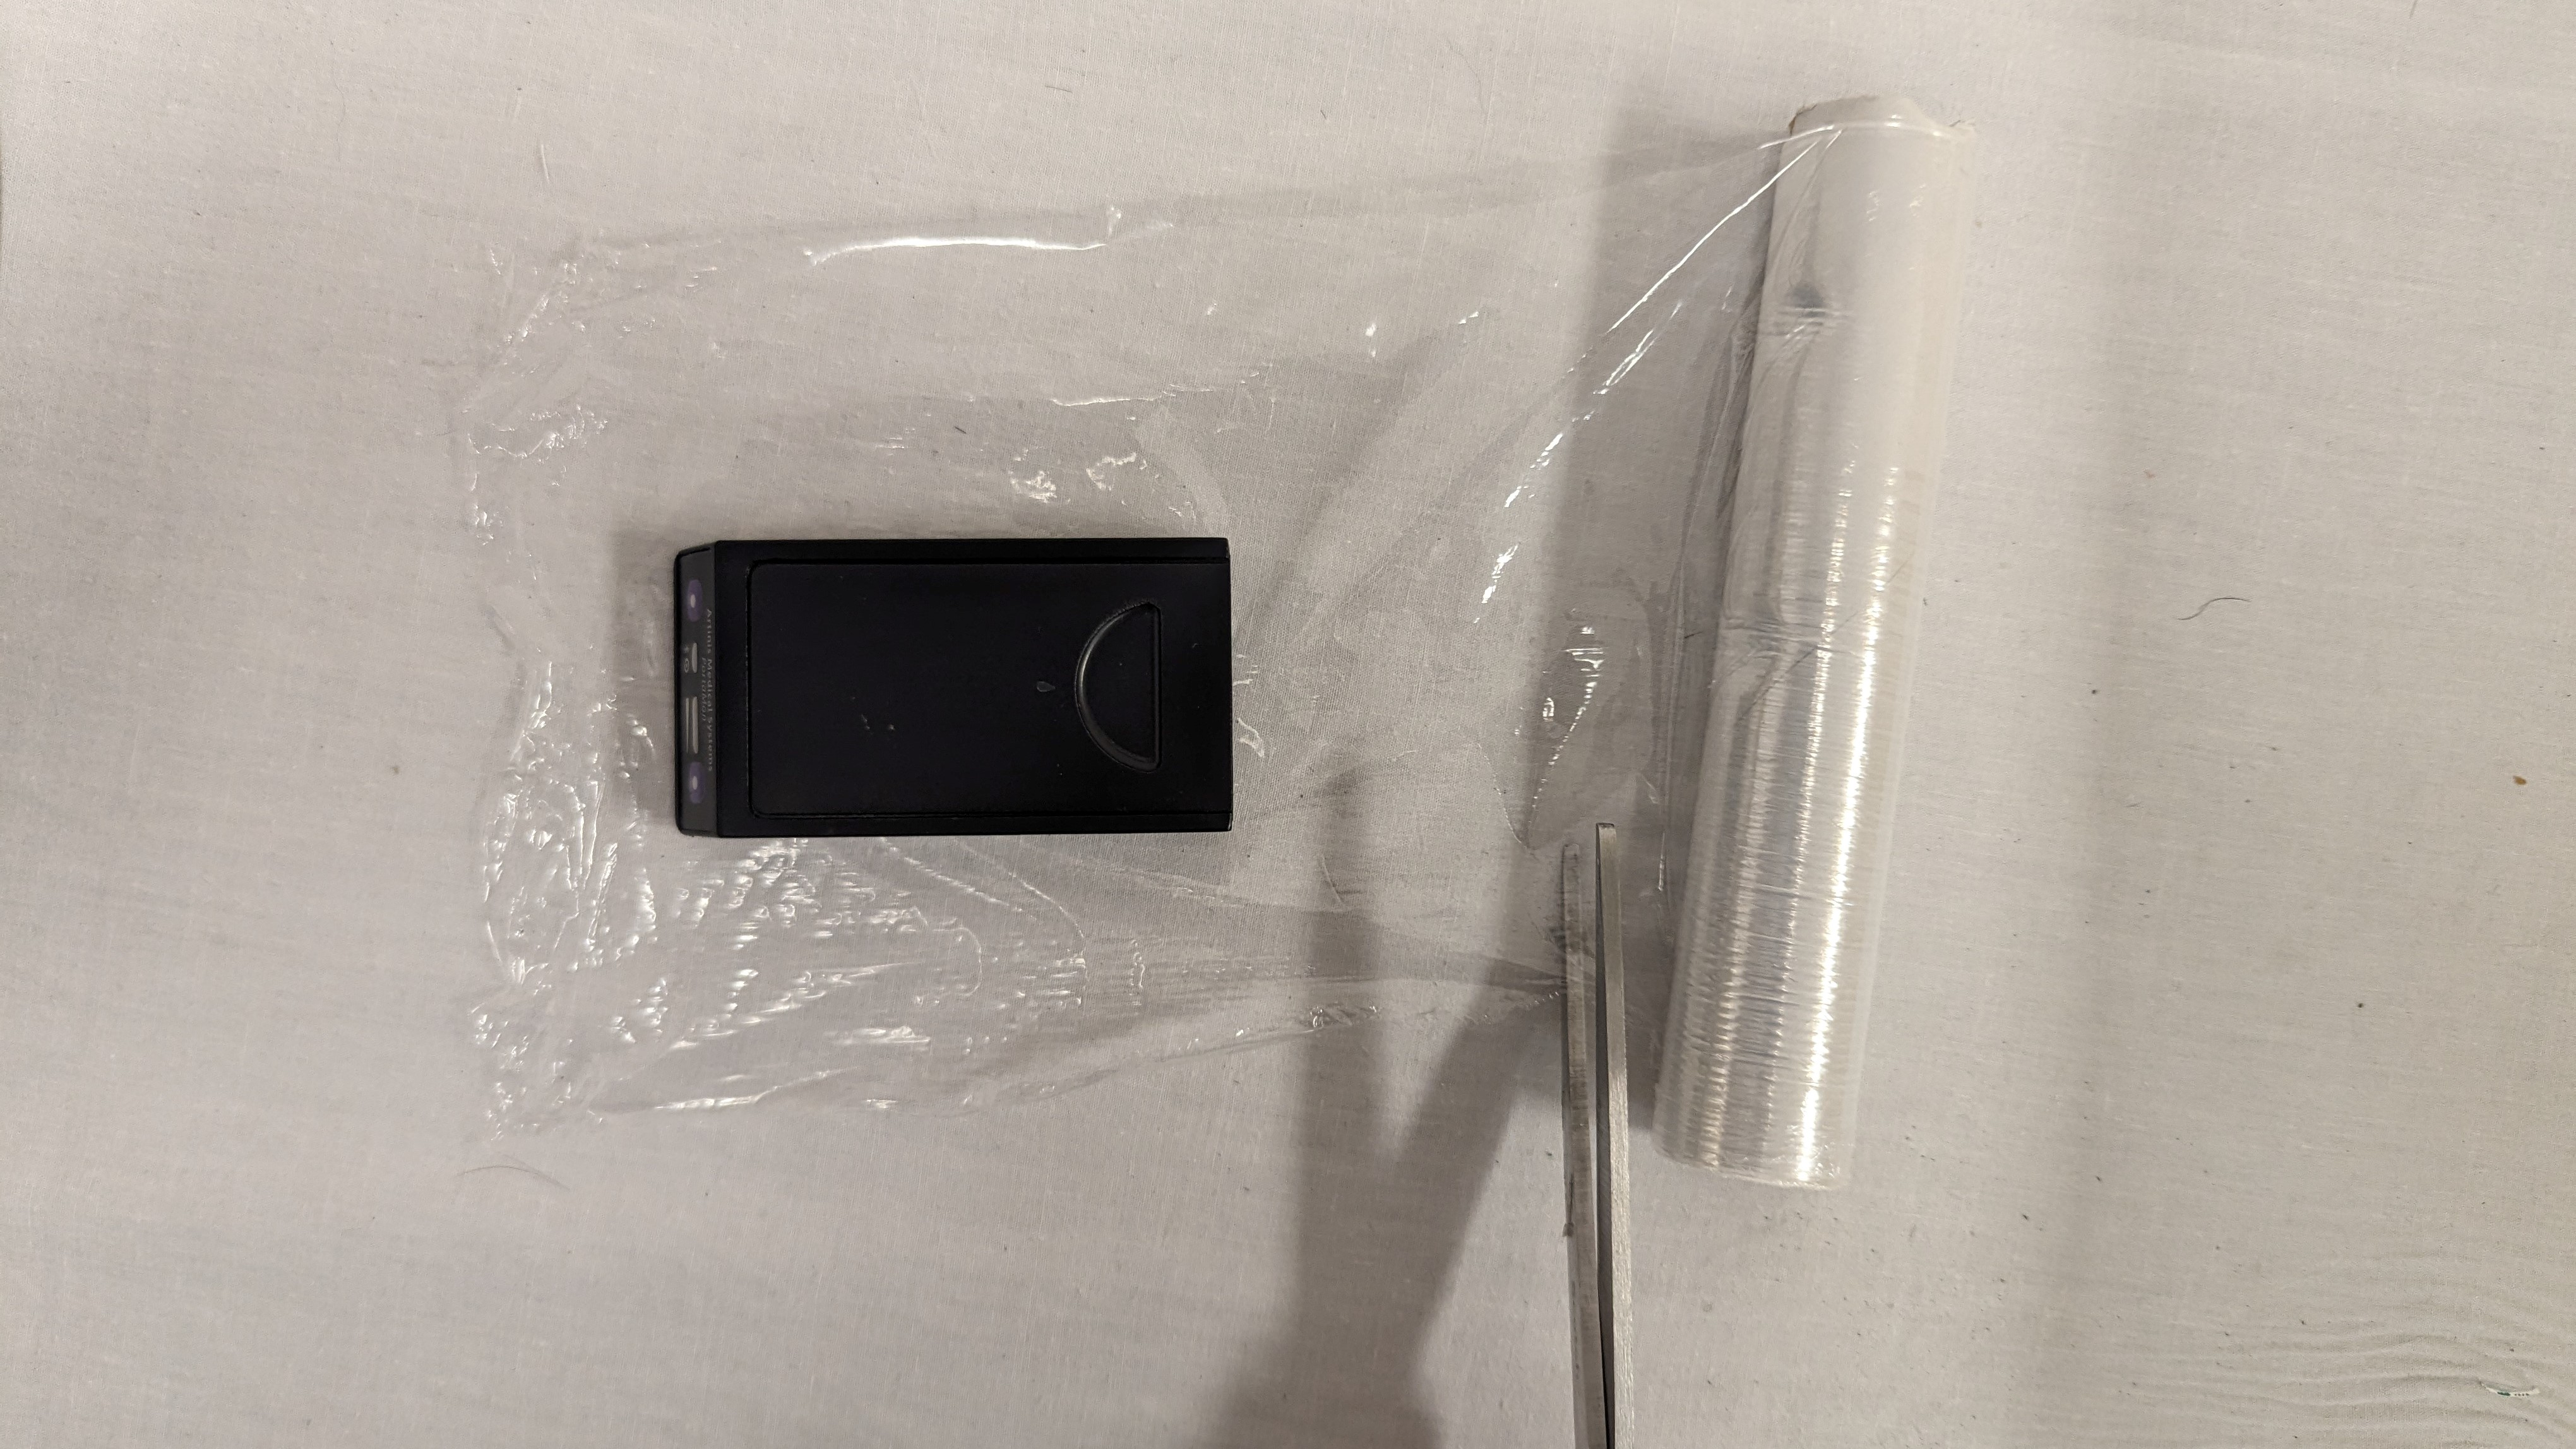
\includegraphics[width=0.33\linewidth]{images/portamon/saranwrapsize}
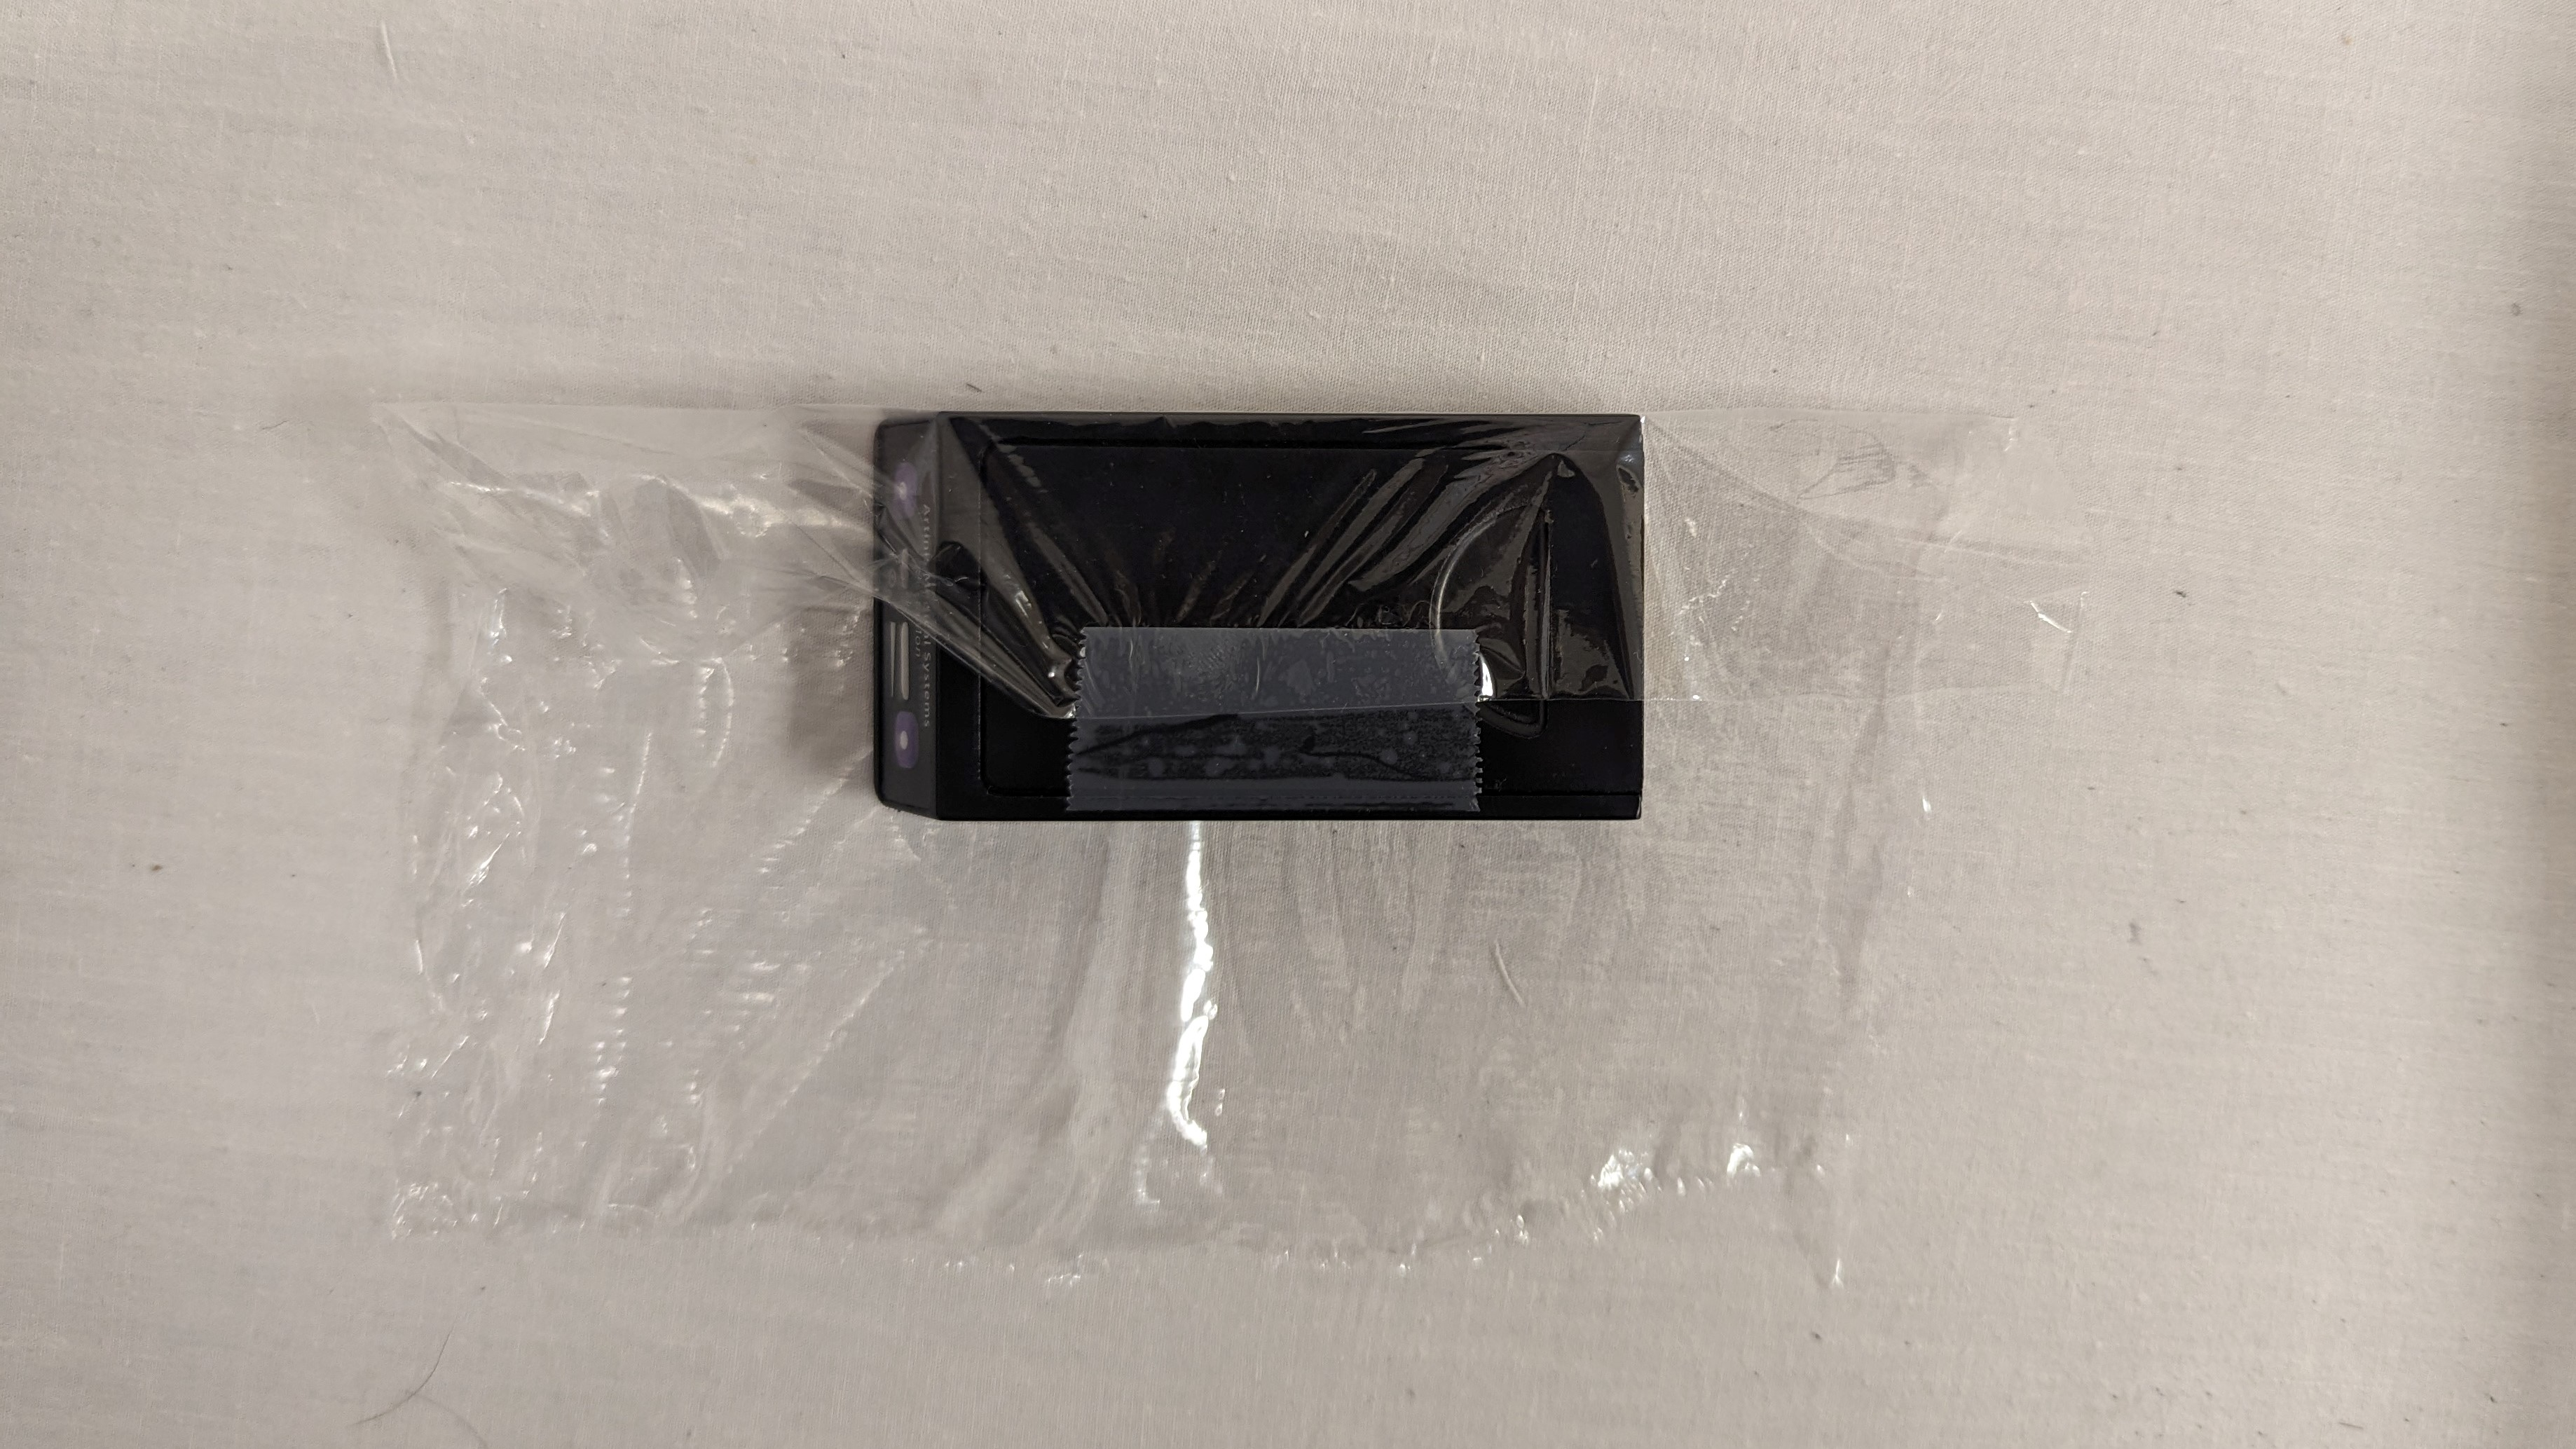
\includegraphics[width=0.33\linewidth]{images/portamon/saranwraponeside}
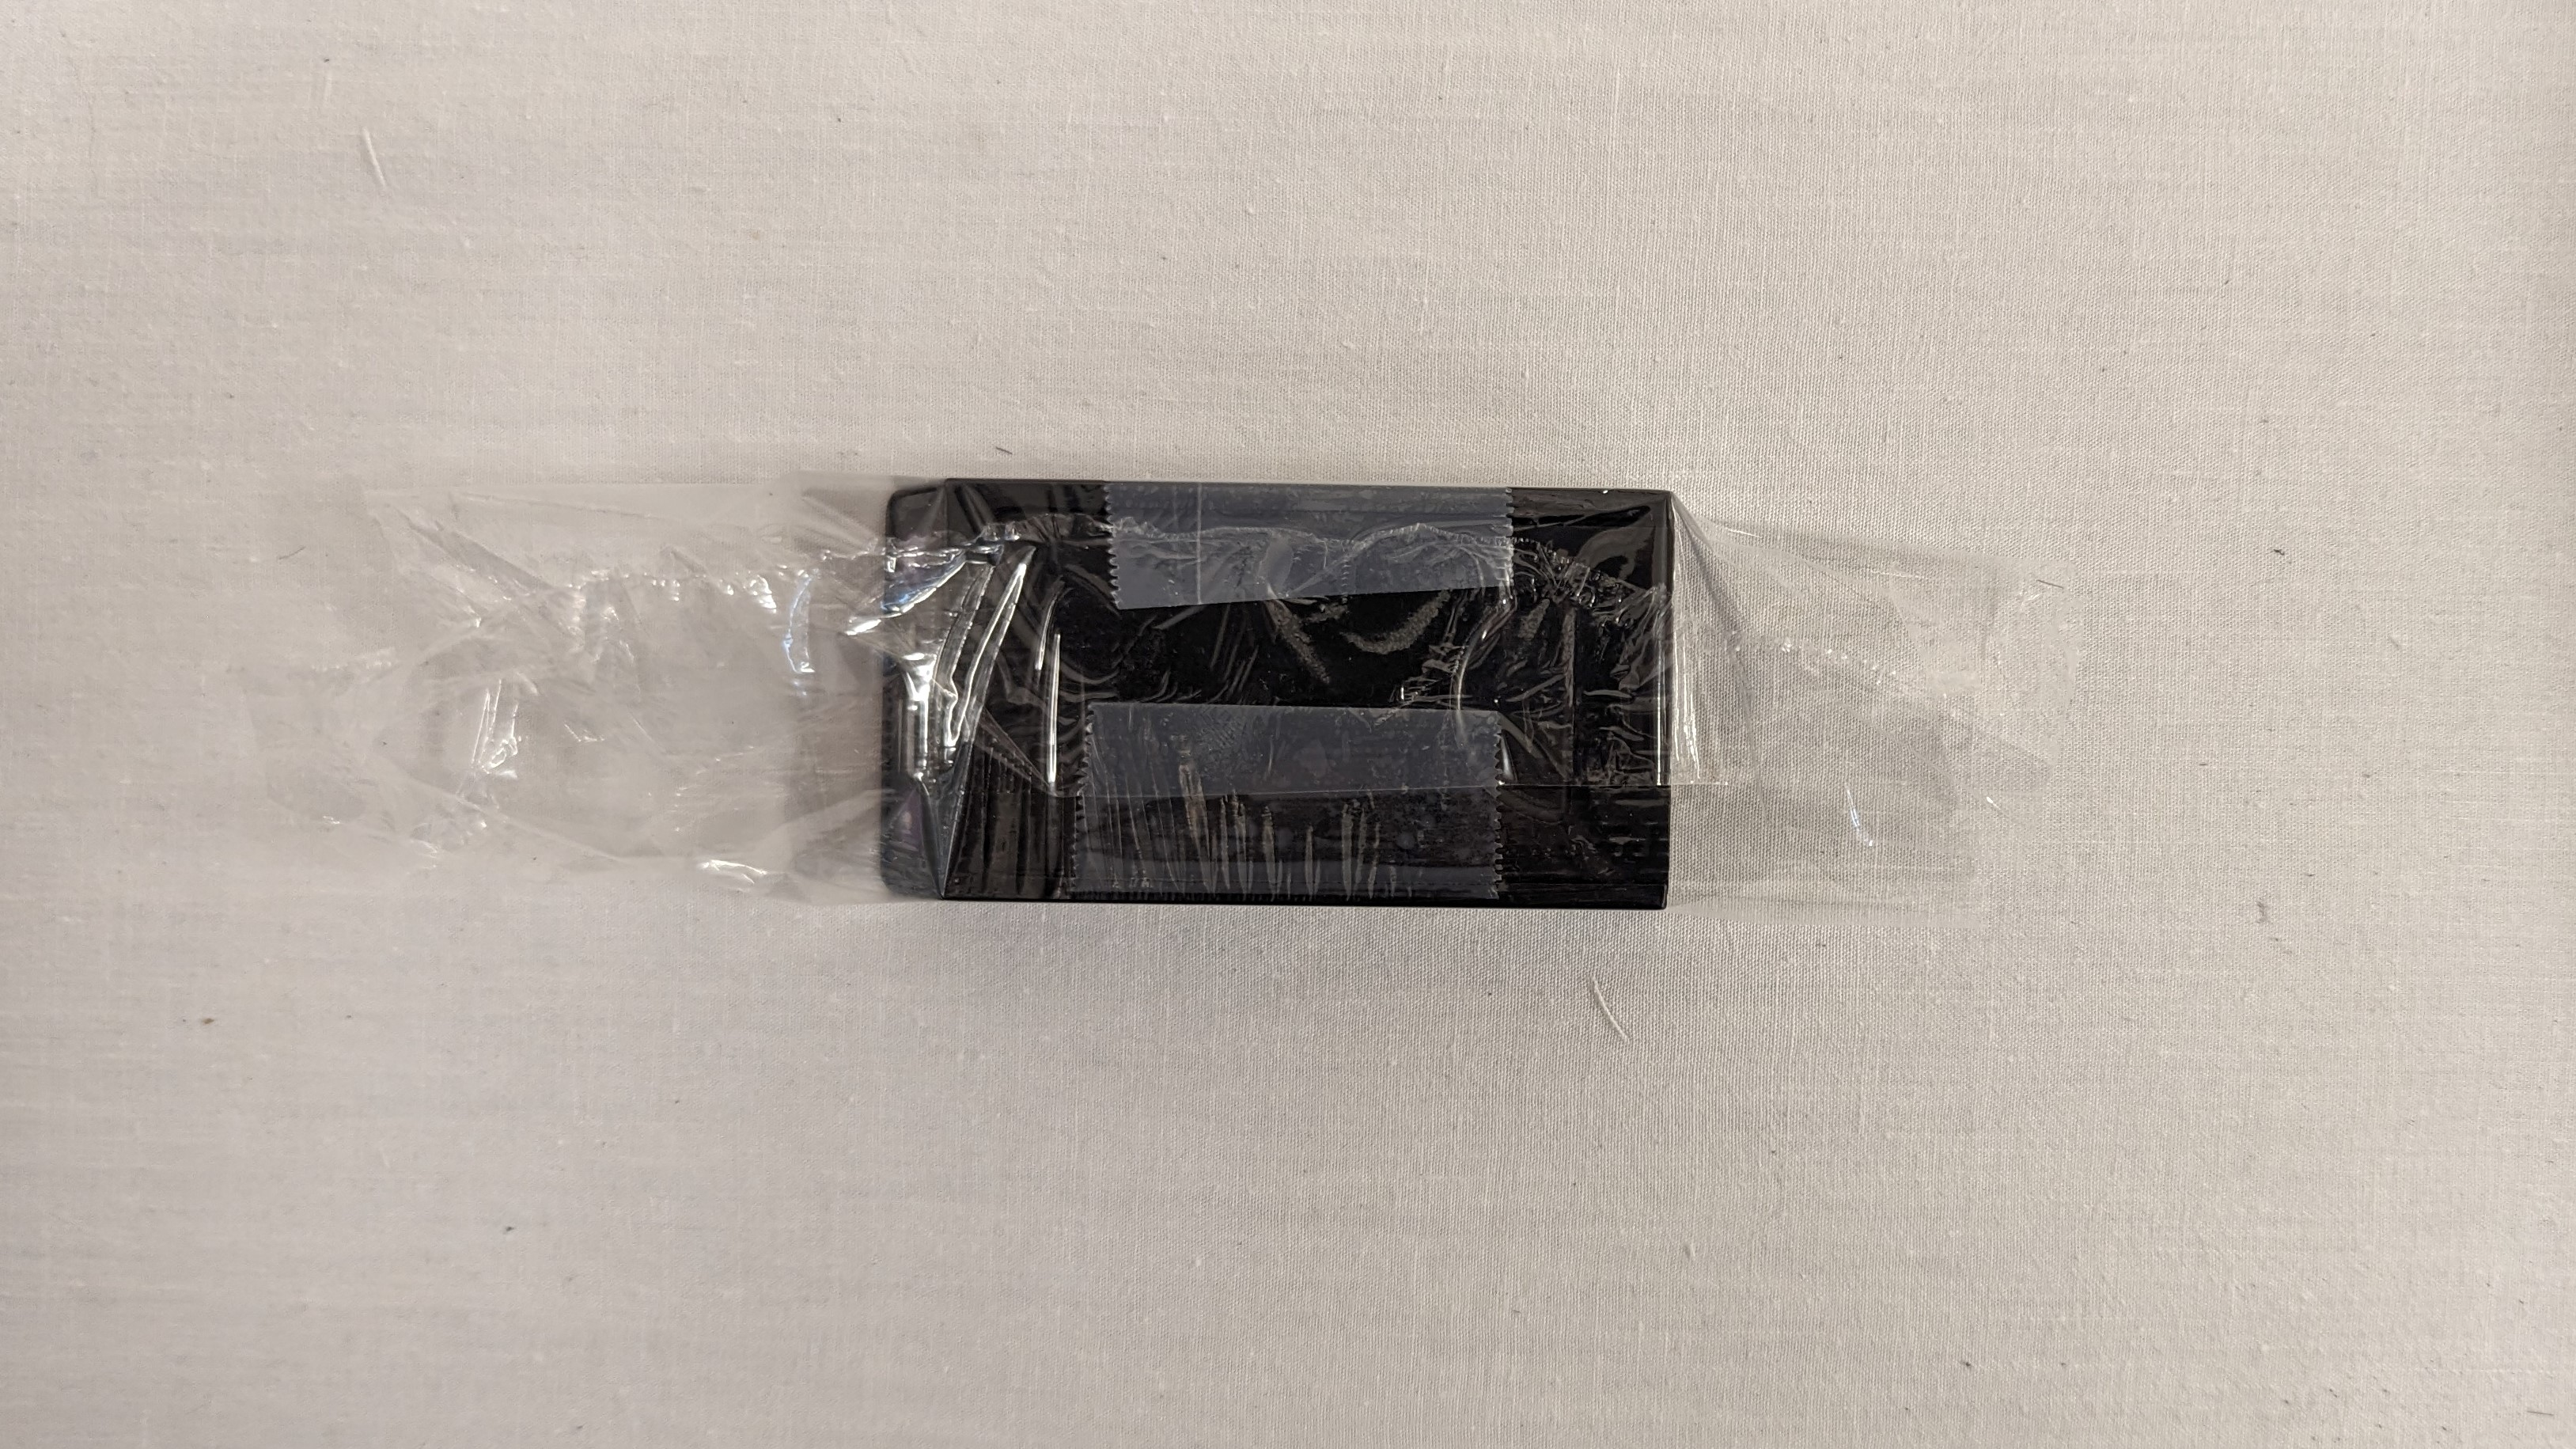
\includegraphics[width=0.33\linewidth]{images/portamon/saranwrapbothsides}

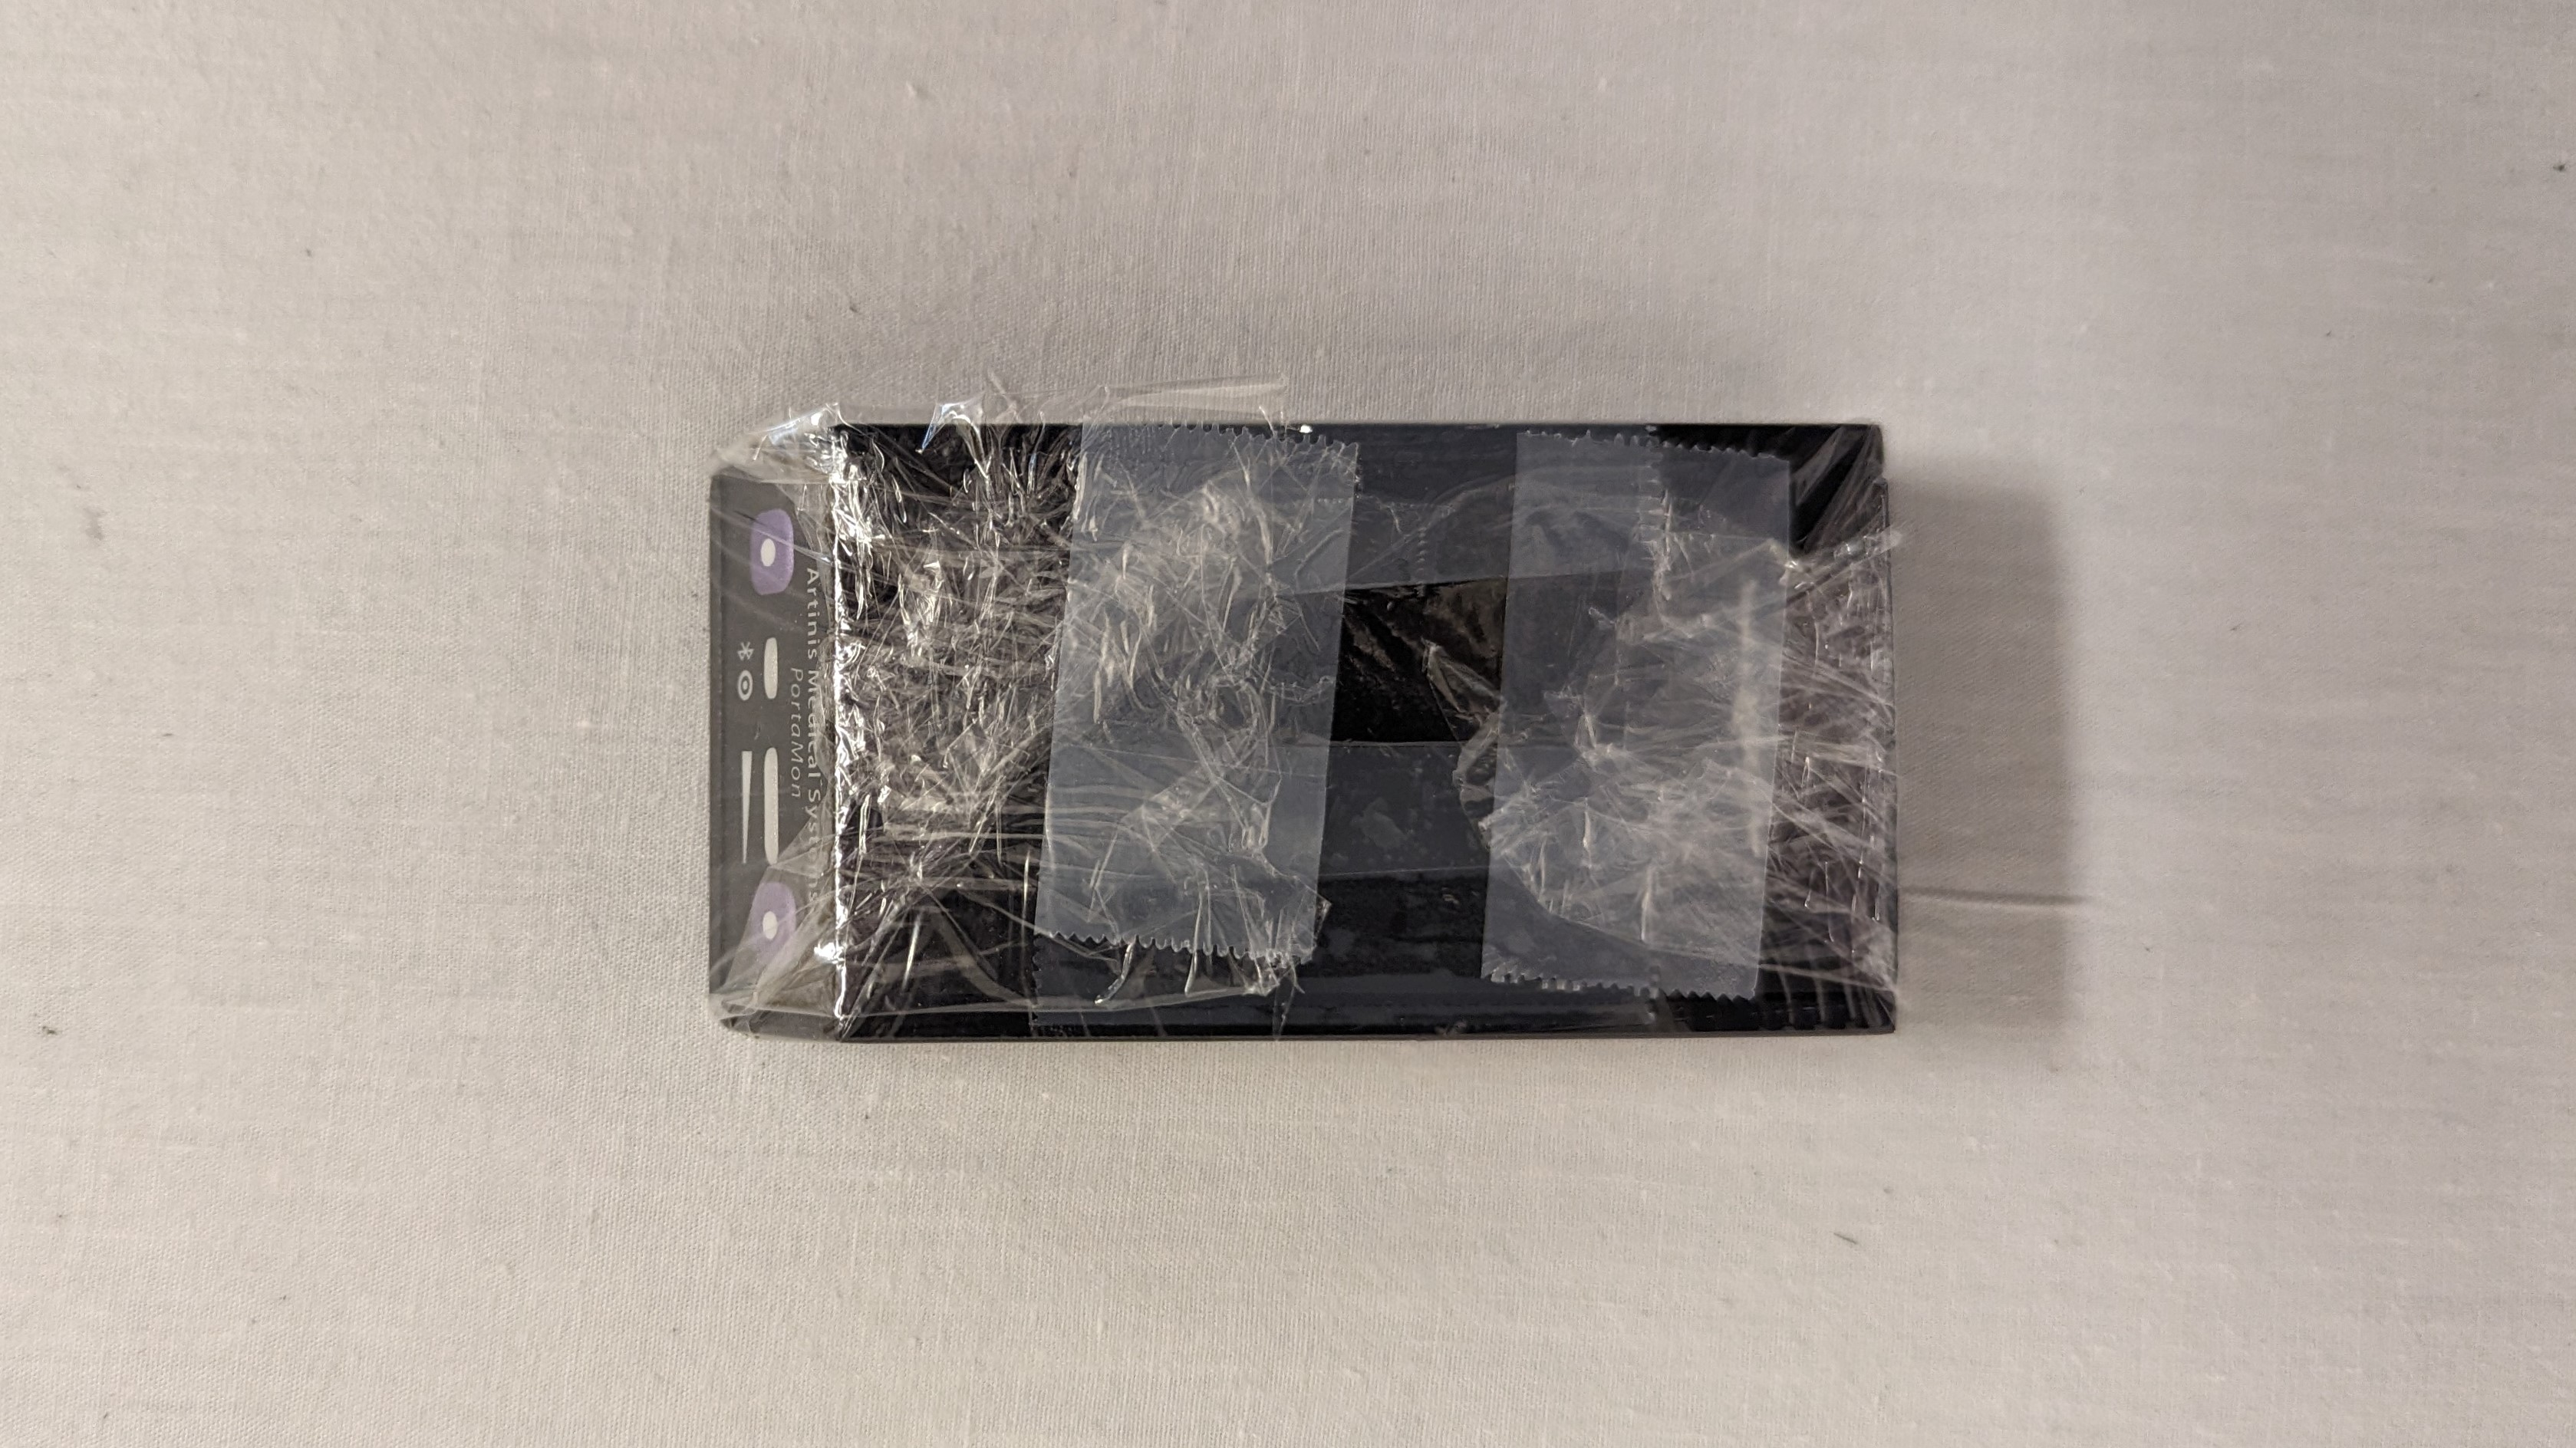
\includegraphics[width=0.5\linewidth]{images/portamon/saranwrapdonetopview}
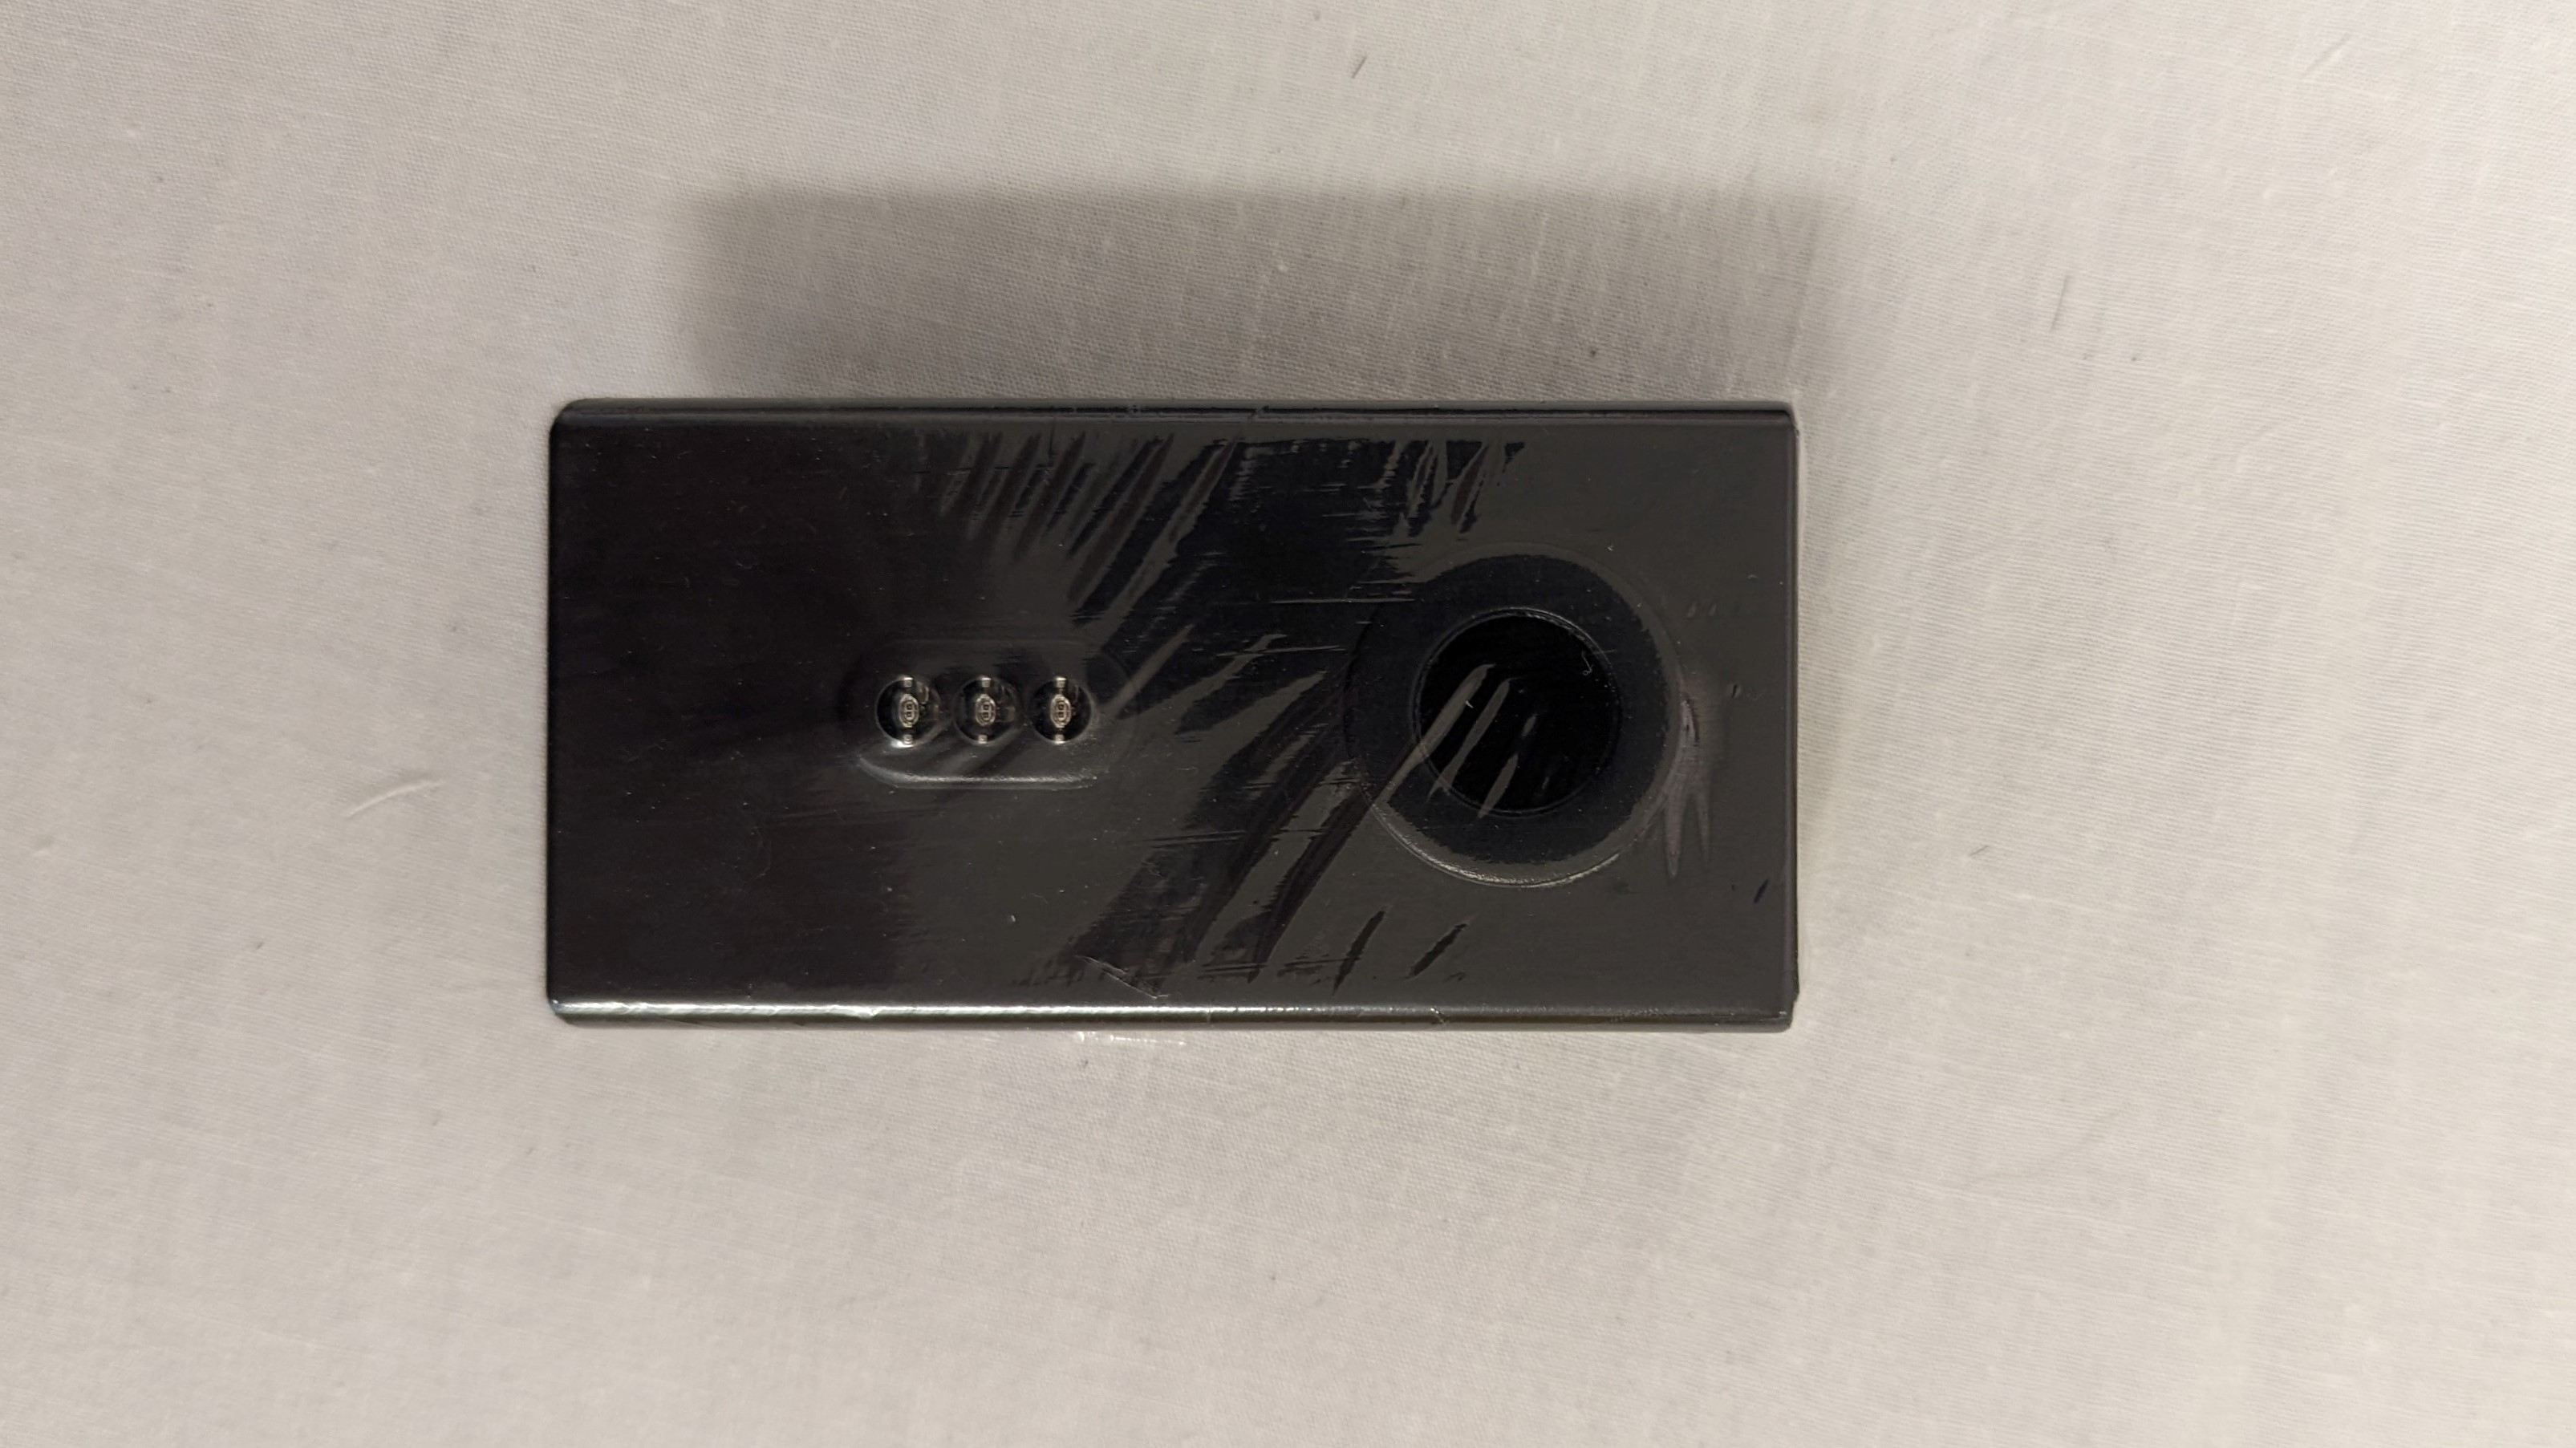
\includegraphics[width=0.5\linewidth]{images/portamon/saranwrapdonebottomview}

\begin{itemize}
\tightlist
\item
  Cut the double-sided taupe tape length-wise into two long strips.
\item
  Place one strip to the left of the transmitters and receiver and one strip to the right of the transmitters and receiver. Leave the exterior side of the double-sided tape covered until the placement on the thigh is complete.
\end{itemize}

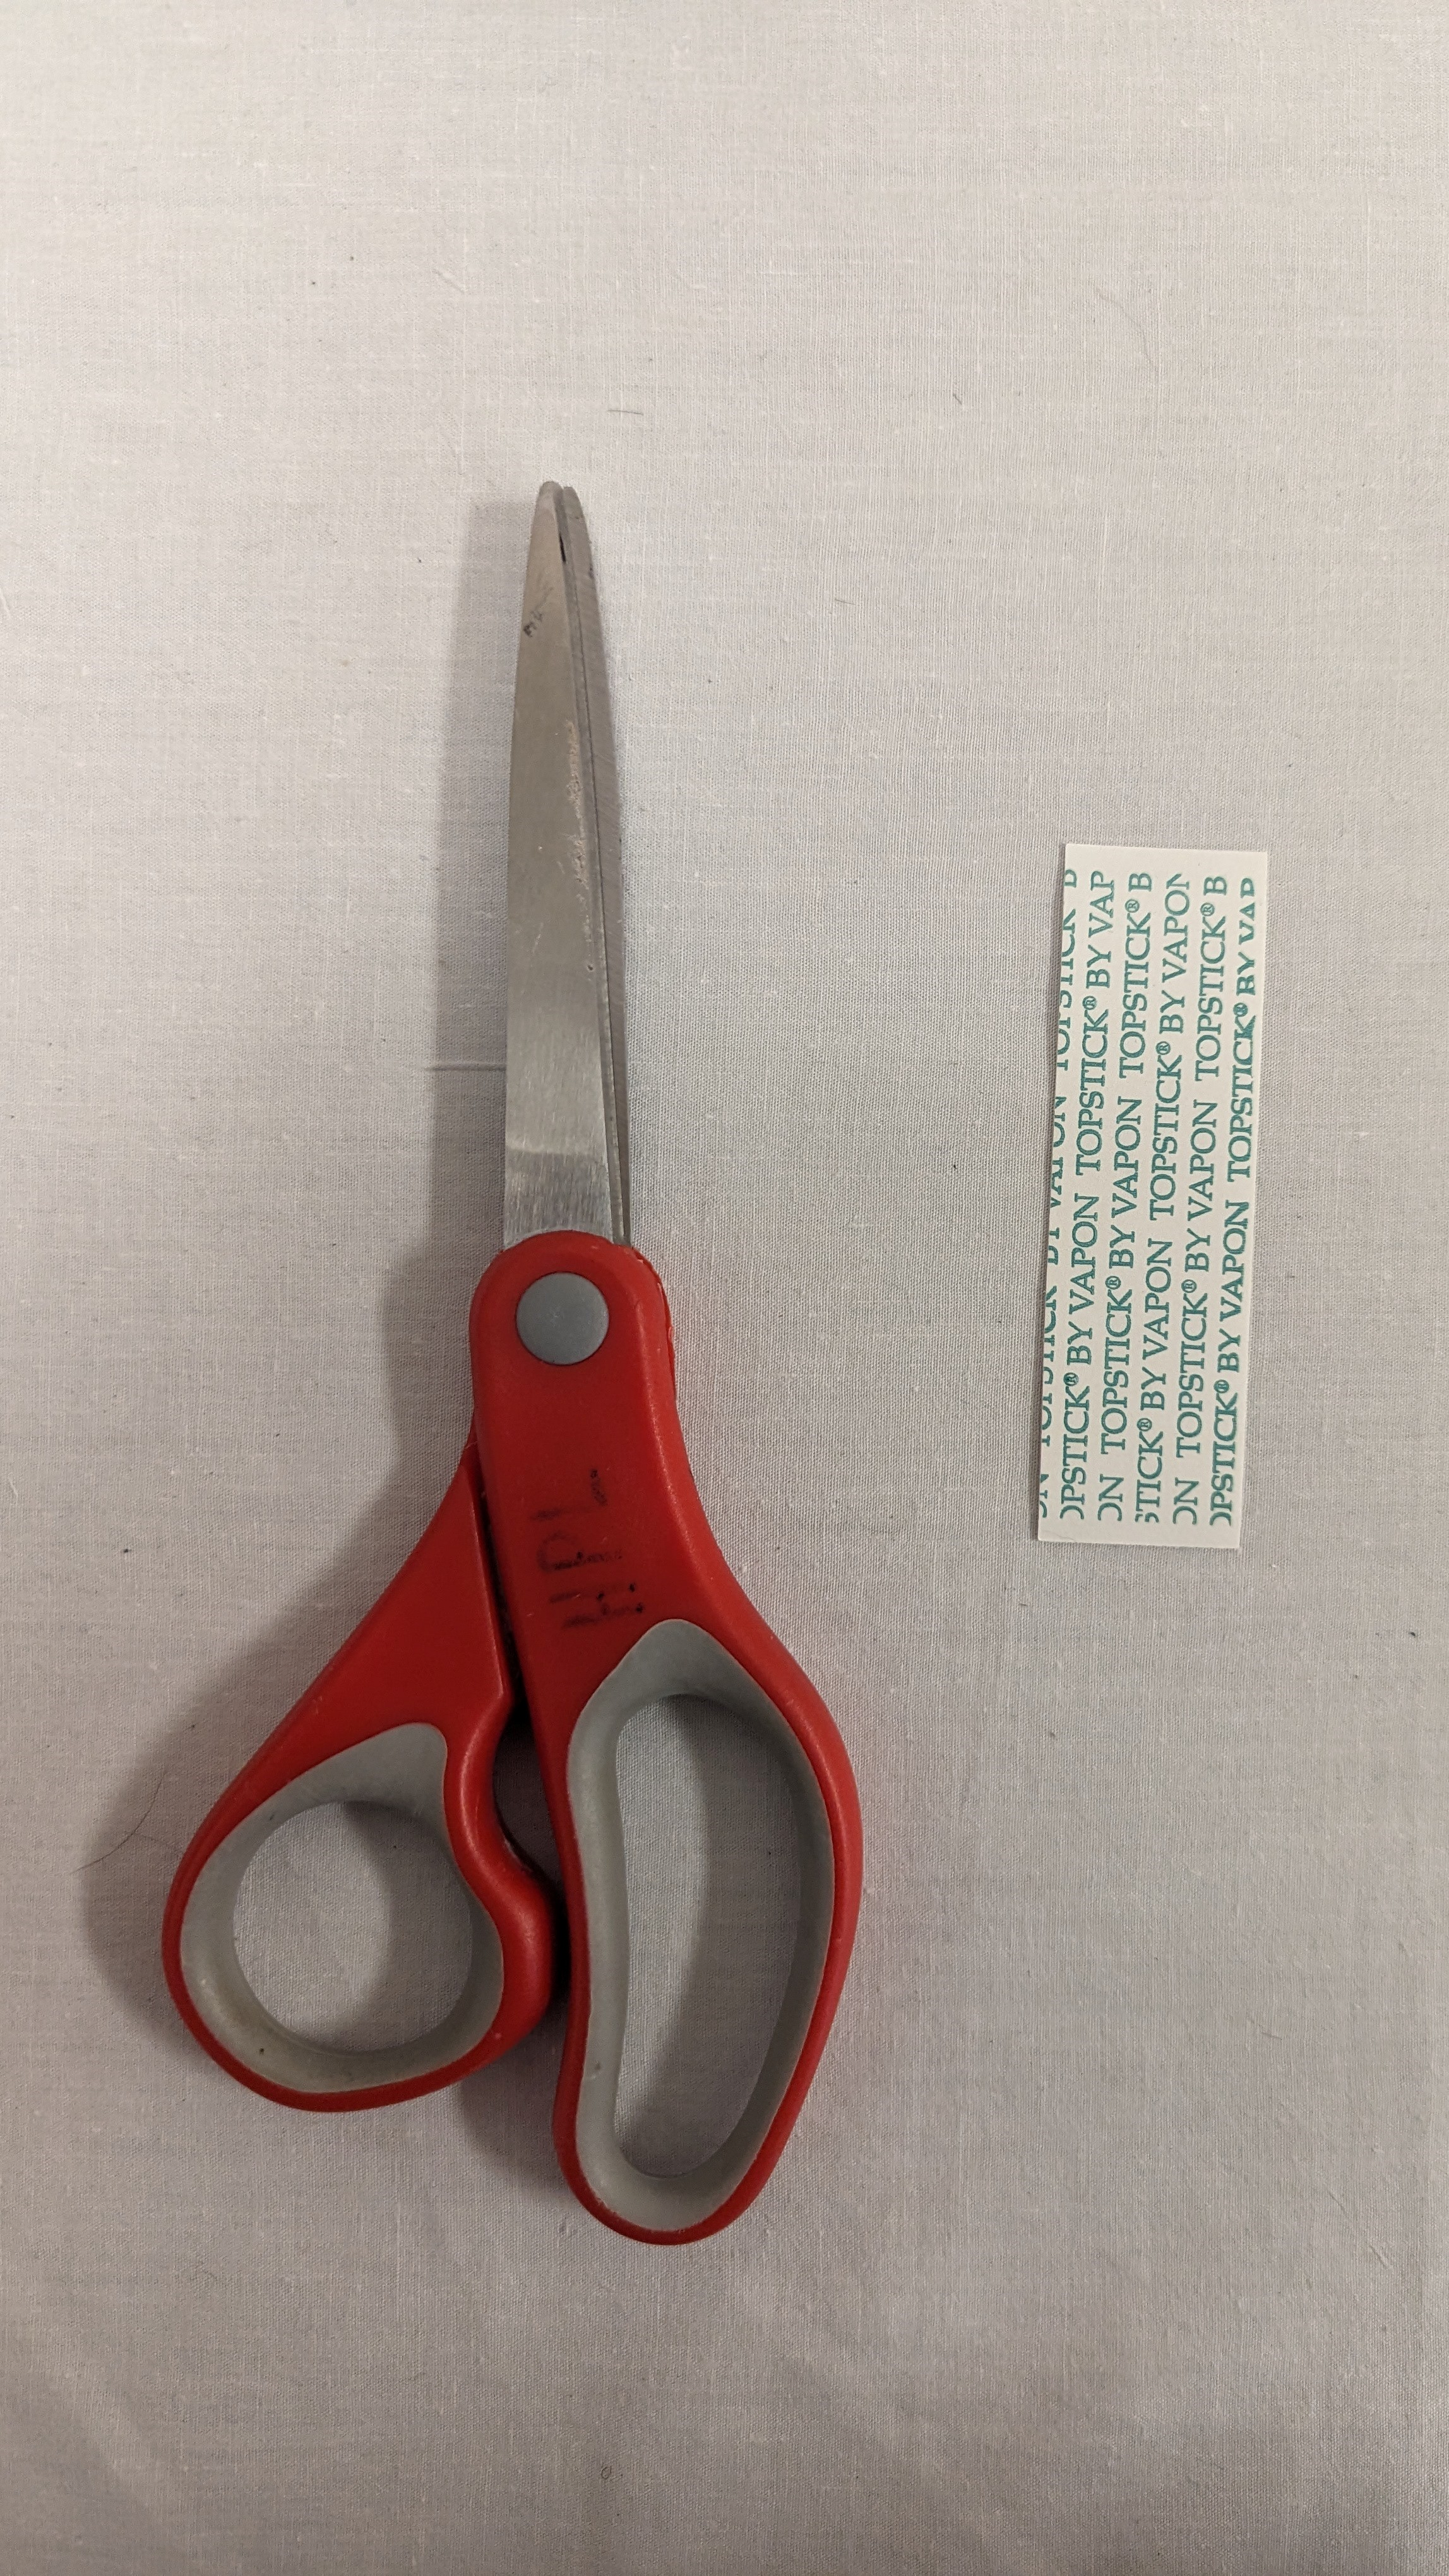
\includegraphics[width=0.33\linewidth]{images/portamon/scissorsandtaupetape}
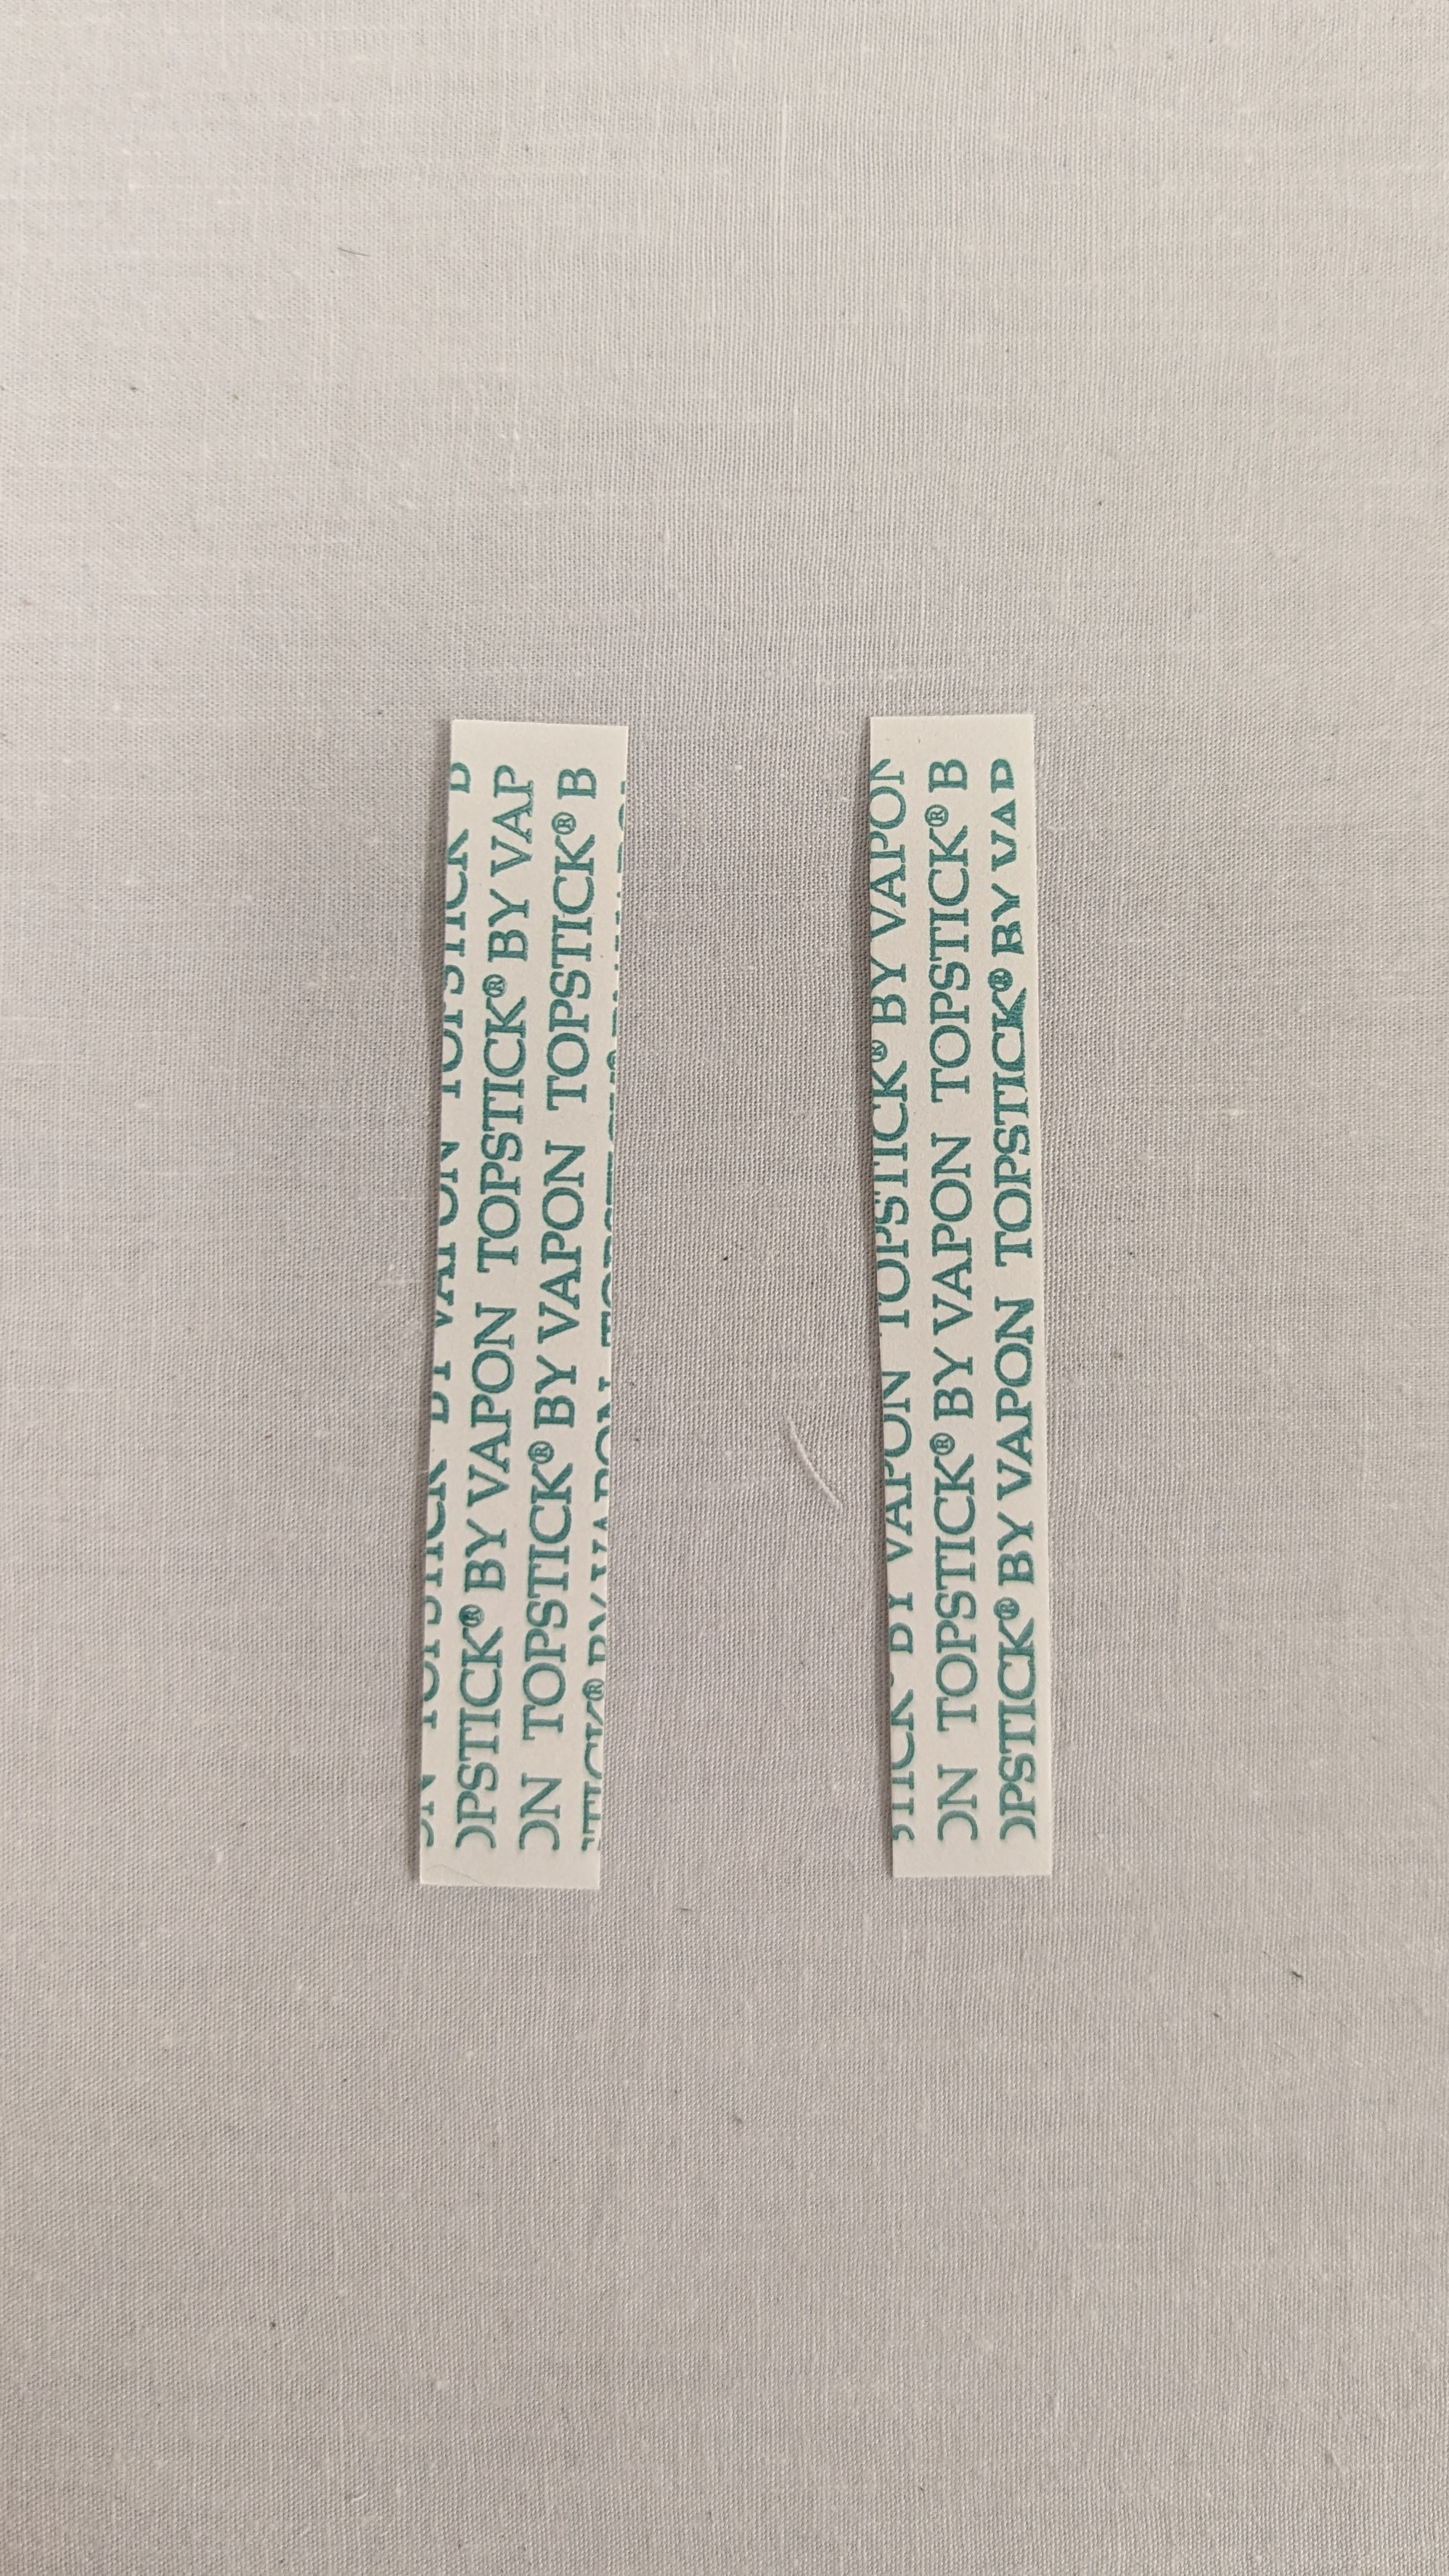
\includegraphics[width=0.33\linewidth]{images/portamon/taupetapelongsplit}
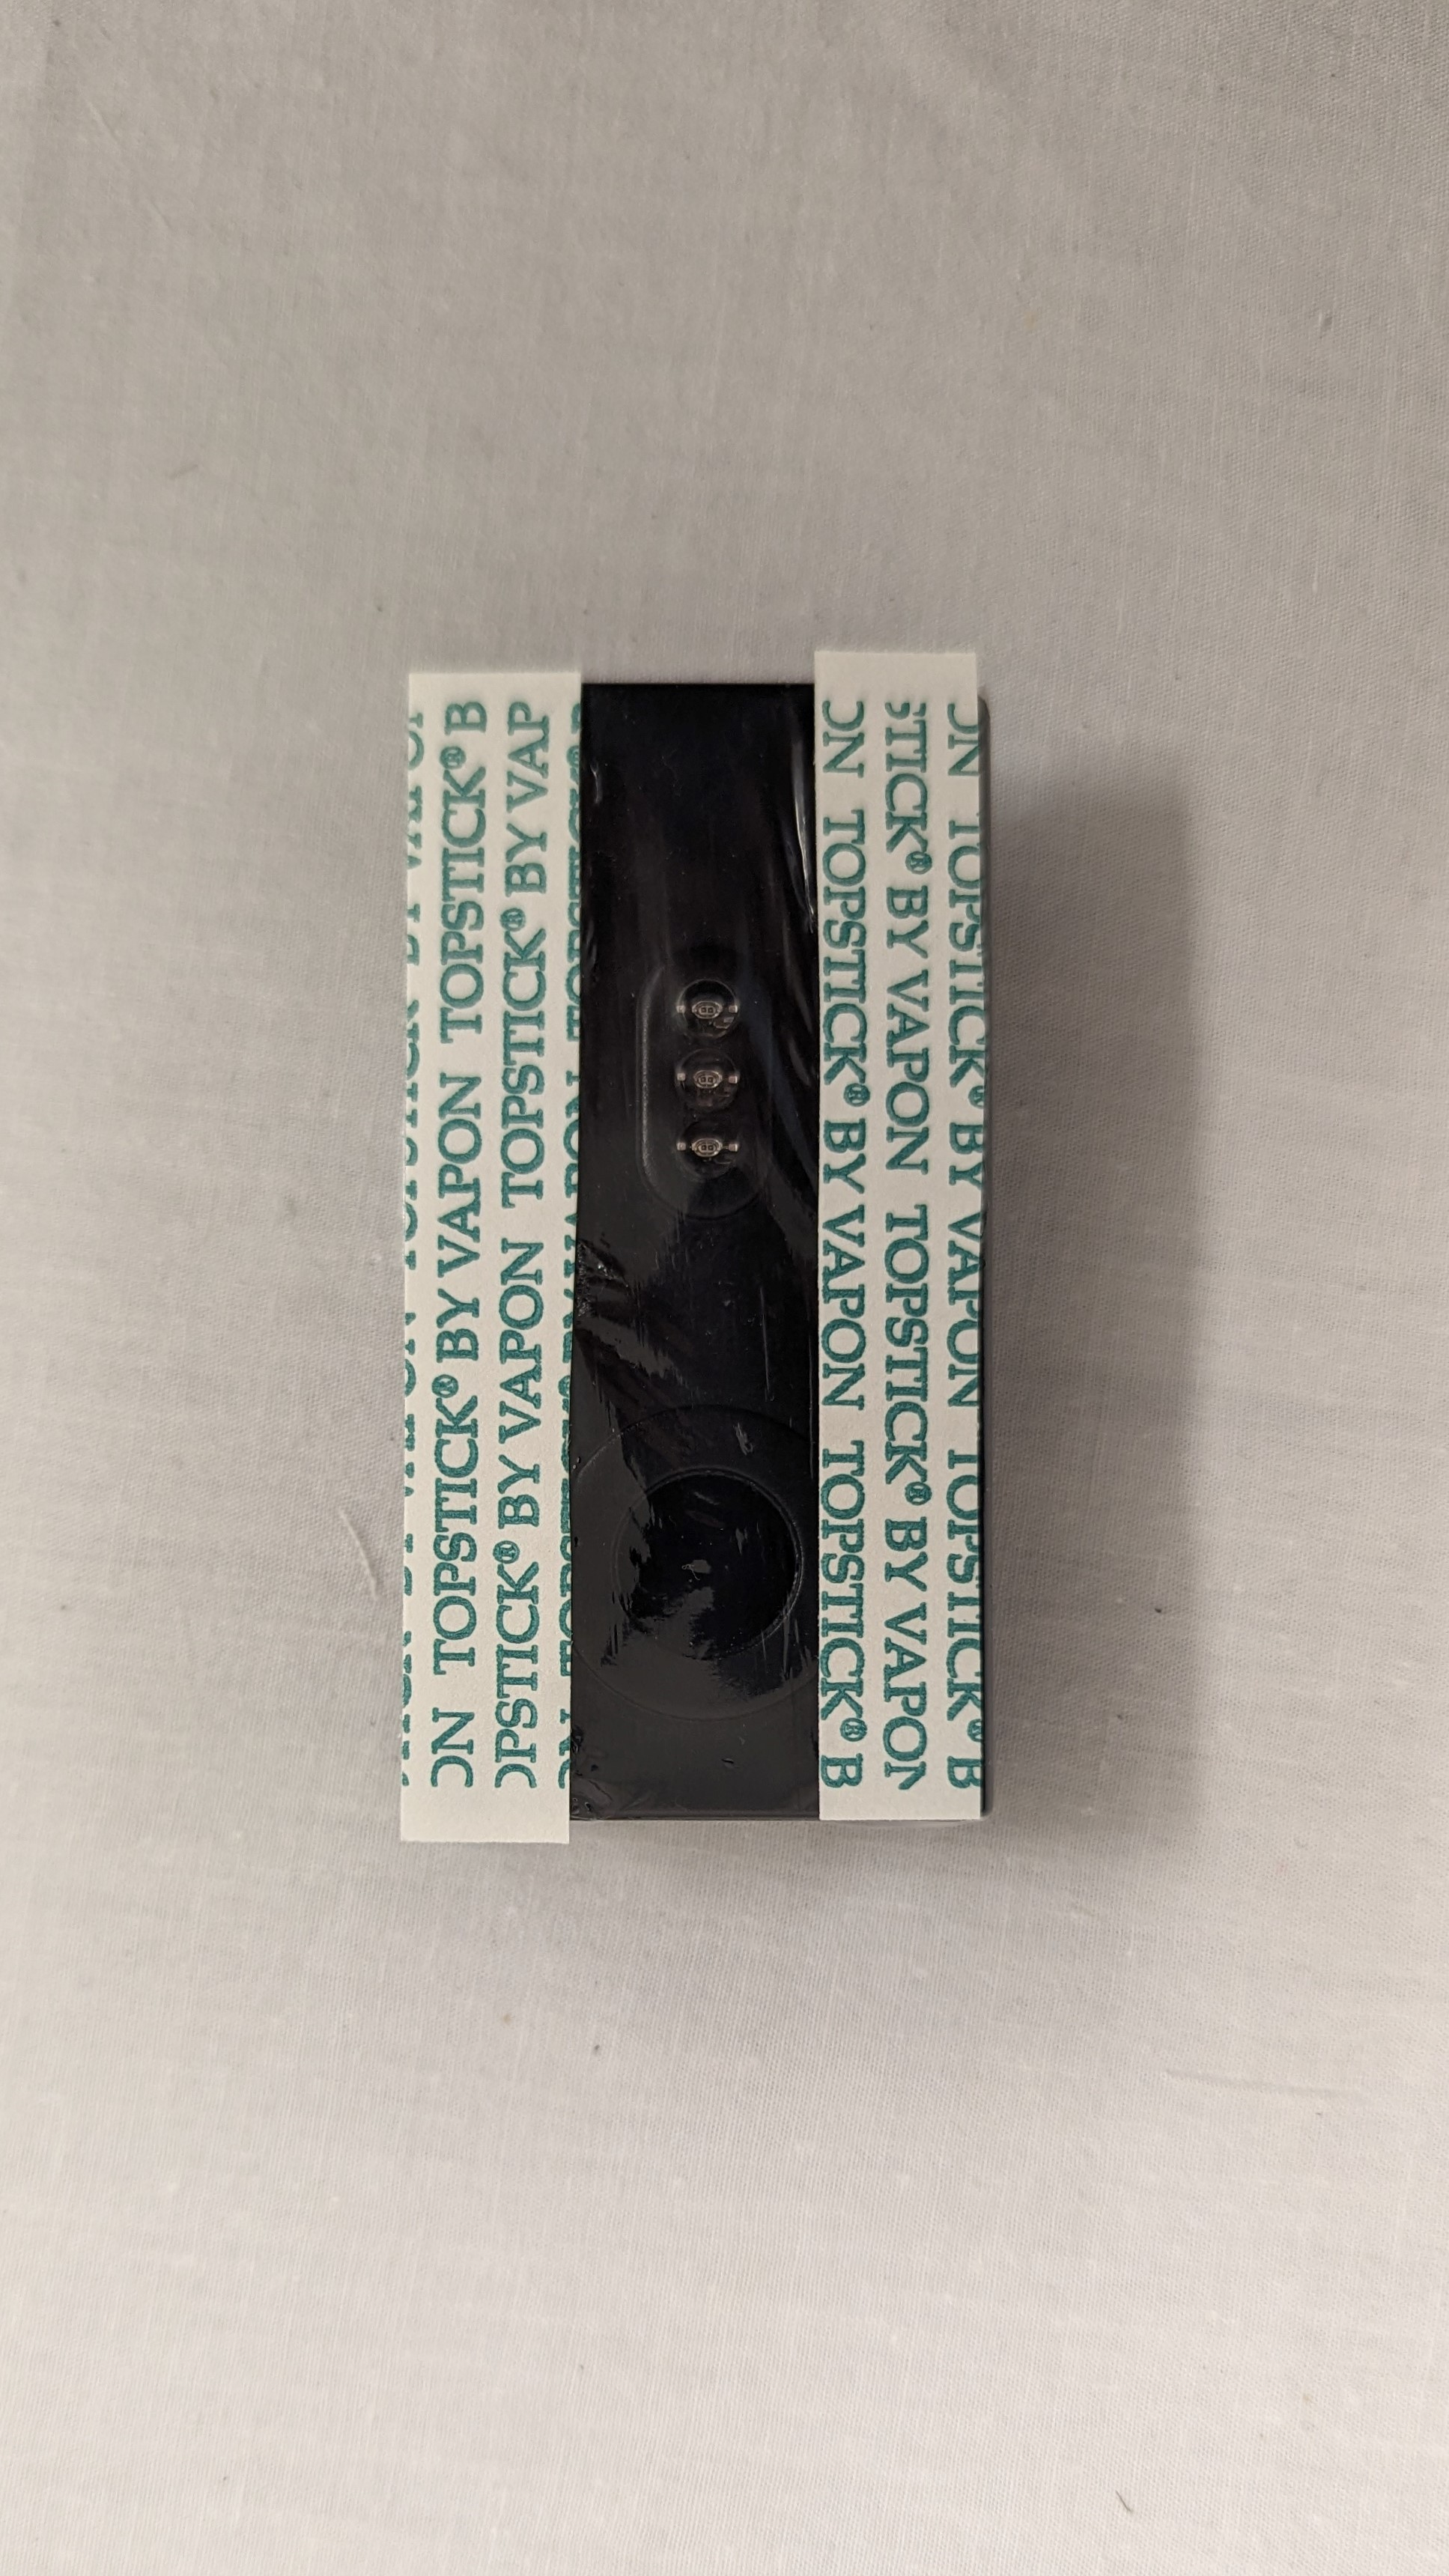
\includegraphics[width=0.33\linewidth]{images/portamon/taupetapeonportamon}

\hypertarget{bluetooth-troubleshooting}{%
\subsection{Bluetooth Troubleshooting}\label{bluetooth-troubleshooting}}

\hypertarget{PortaMon-StartMeasurement}{%
\subsection{Start a Measurement}\label{PortaMon-StartMeasurement}}

\begin{itemize}
\tightlist
\item
  Turn on the ASUS laptop.\\
\item
  Ensure the bluetooth dongle and the Rockey dongle are plugged in to the laptop.

  \begin{itemize}
  \tightlist
  \item
    The Rockey license key must say `ROCKEY4ND' and NOT `ROCKEY4'. The `ROCKEY4' is from an older Artinis device and is not the current license key. You will not be able to use the most up to date Oxysoft software with the incorrect license key.
  \end{itemize}
\end{itemize}

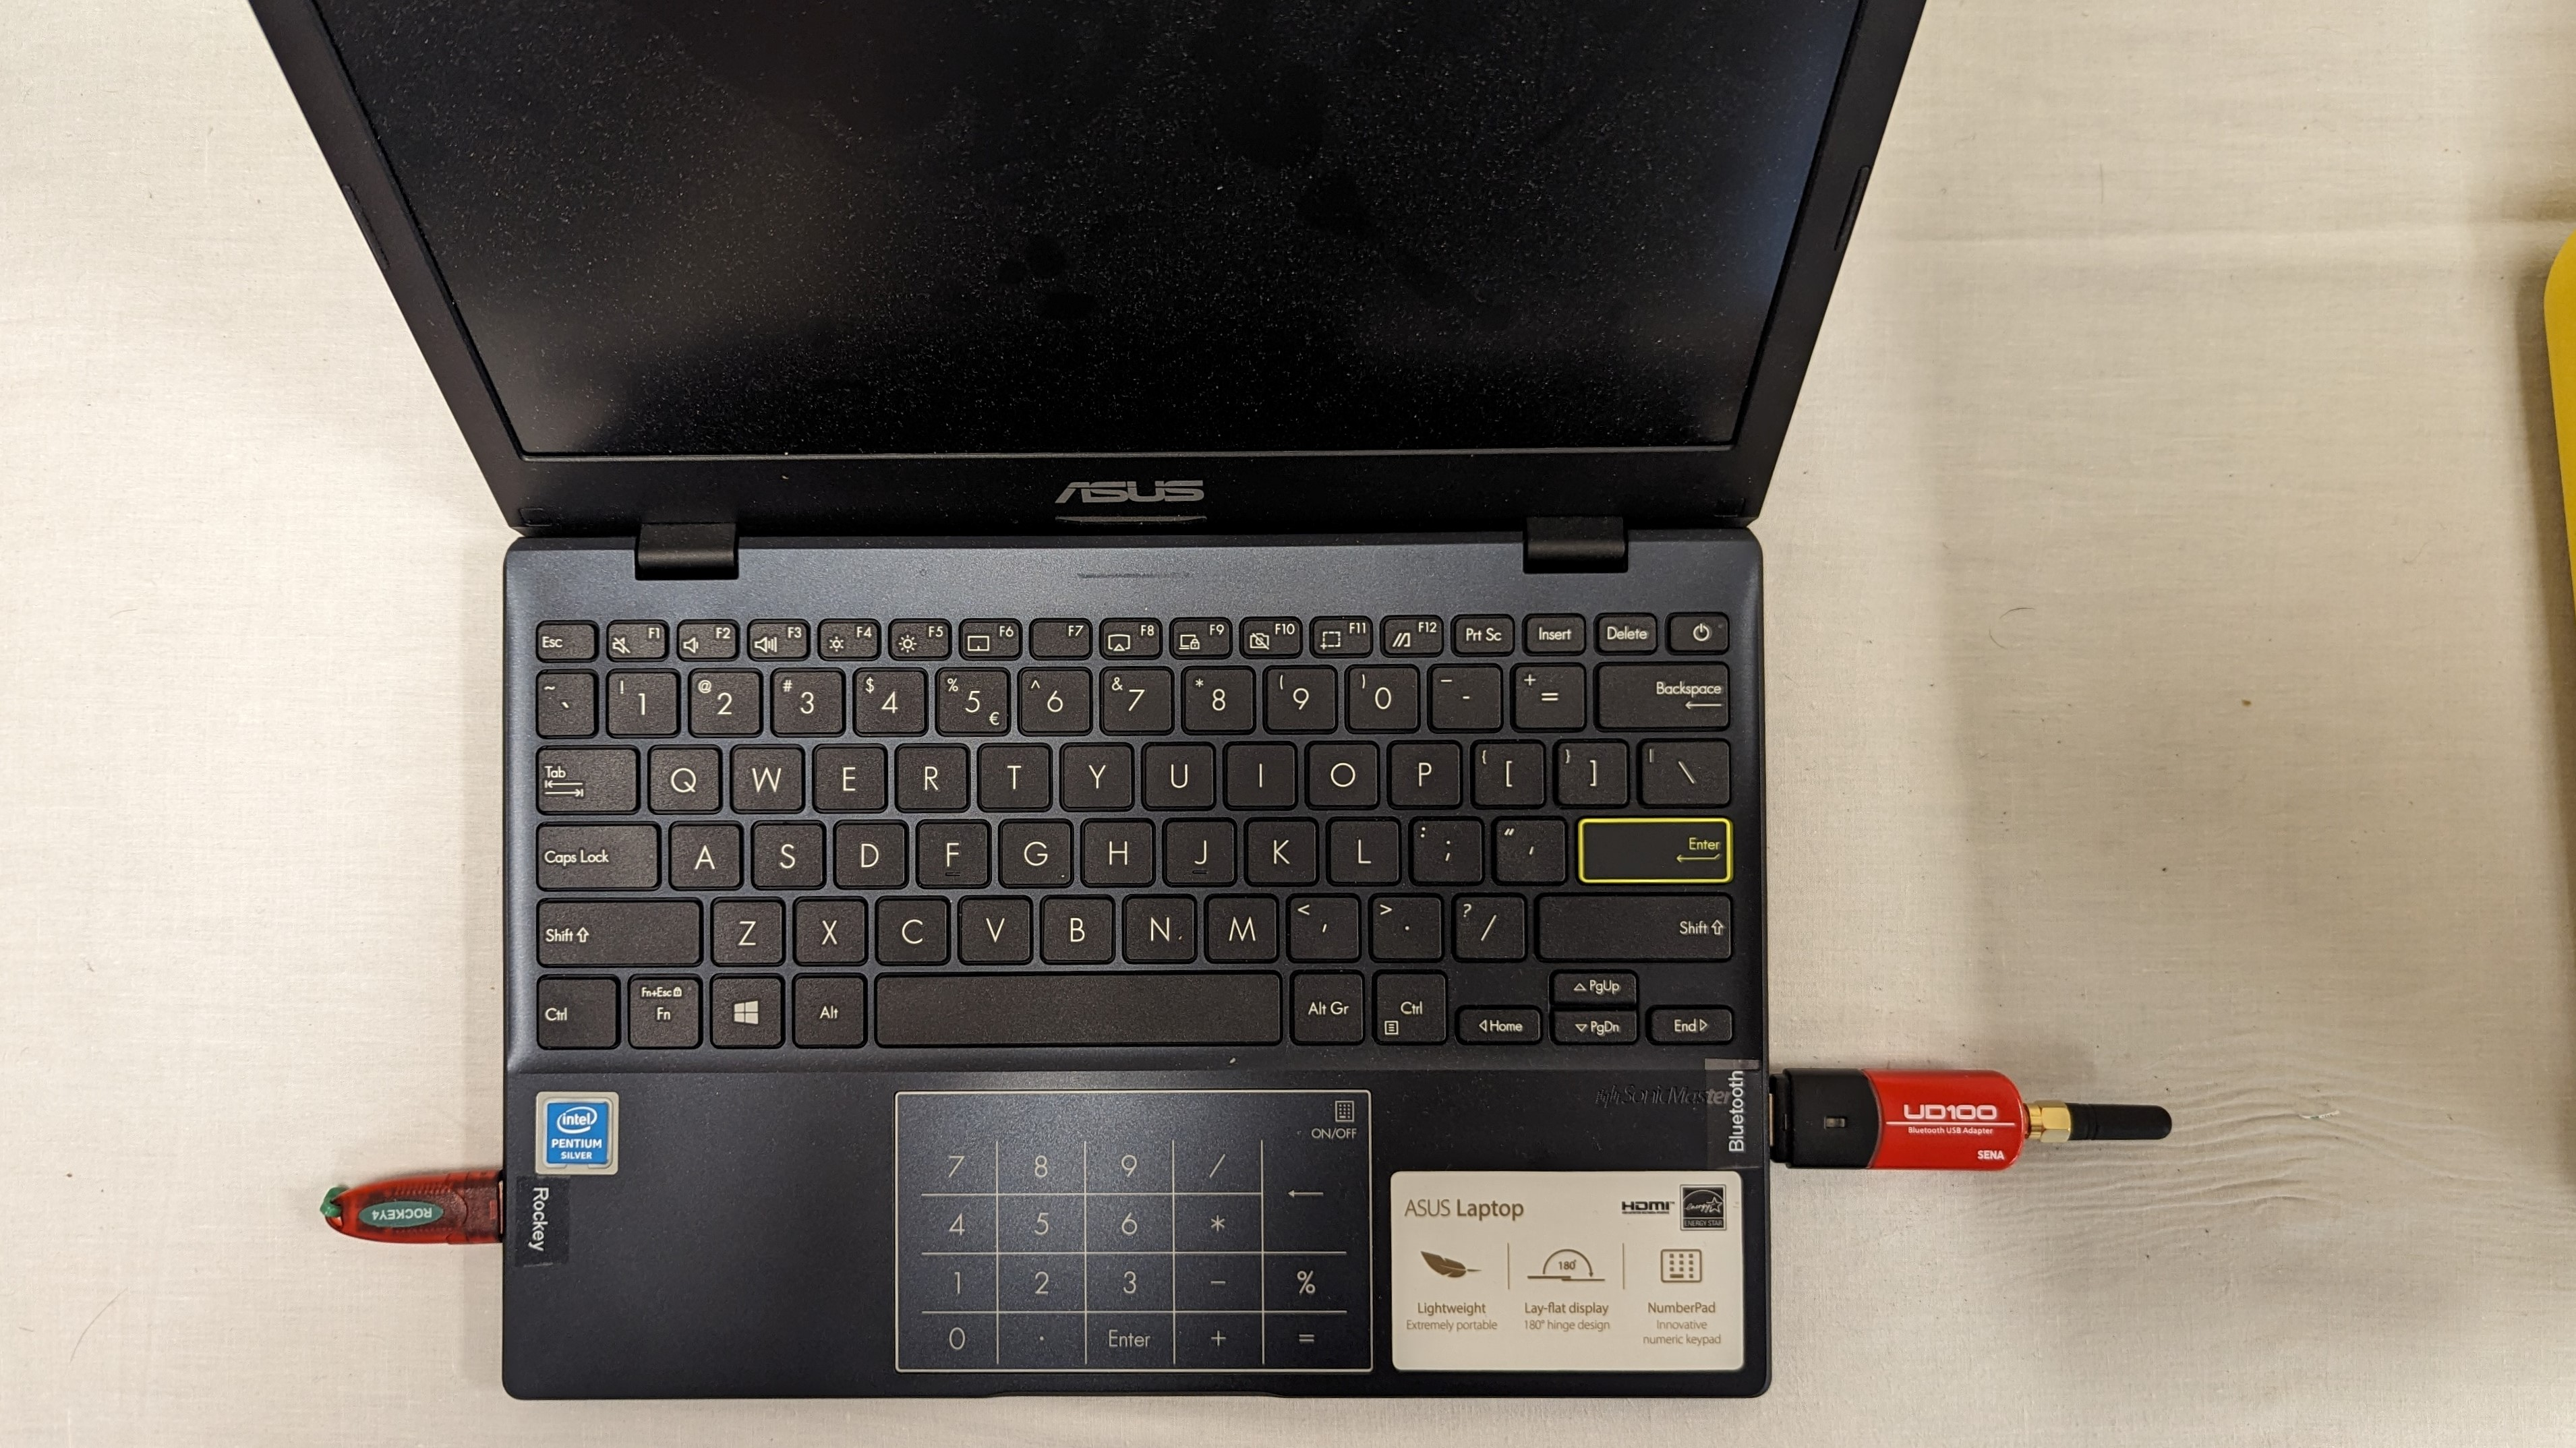
\includegraphics[width=1\linewidth]{images/portamon/laptopwithplugins}

\begin{itemize}
\tightlist
\item
  Open Oxysoft.
\end{itemize}

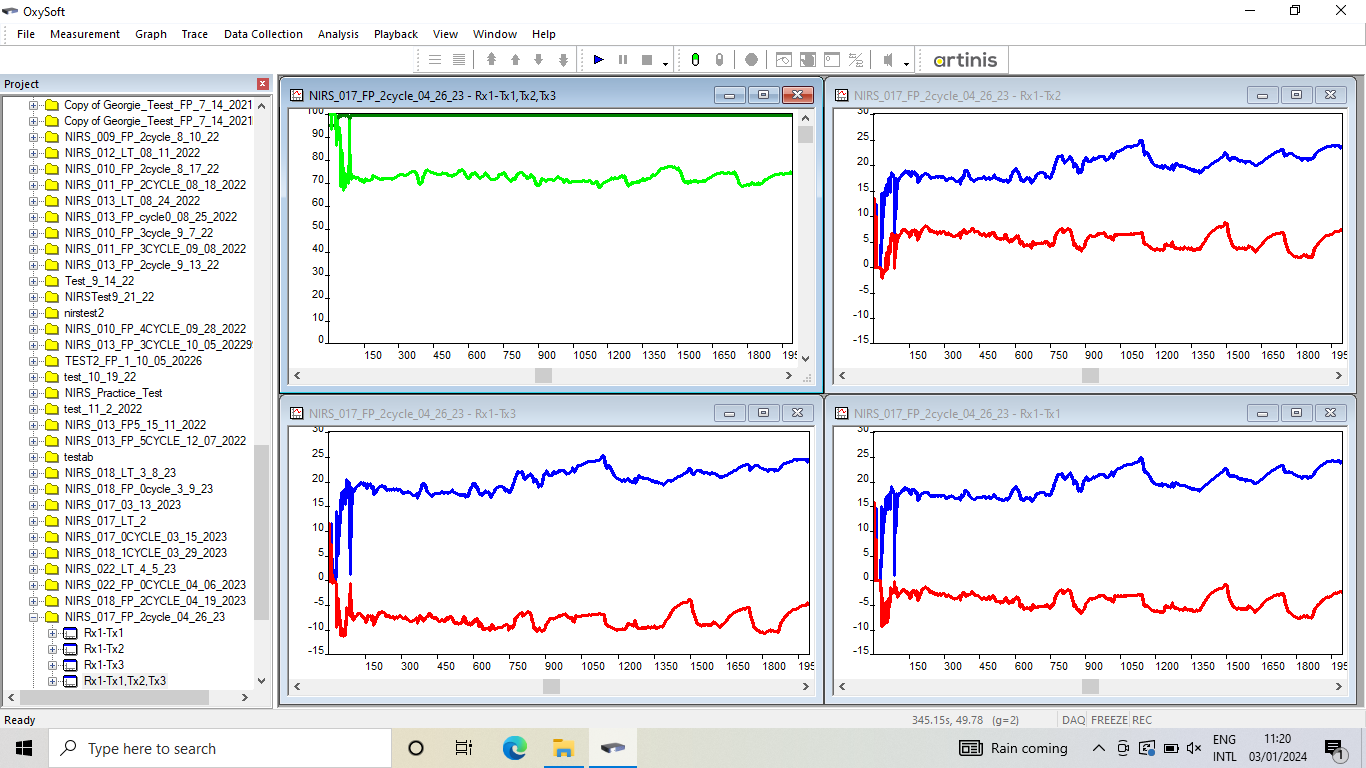
\includegraphics[width=1\linewidth]{images/startnewmeasurement/01_open_oxysoft}

\begin{itemize}
\tightlist
\item
  Close any open graphs in the main panel.

  \begin{itemize}
  \tightlist
  \item
    Select \texttt{Graphs} in the top bar.\\
  \item
    Select \texttt{Close\ all\ graphs}. There should be no open graphs in the main panel.
  \end{itemize}
\end{itemize}

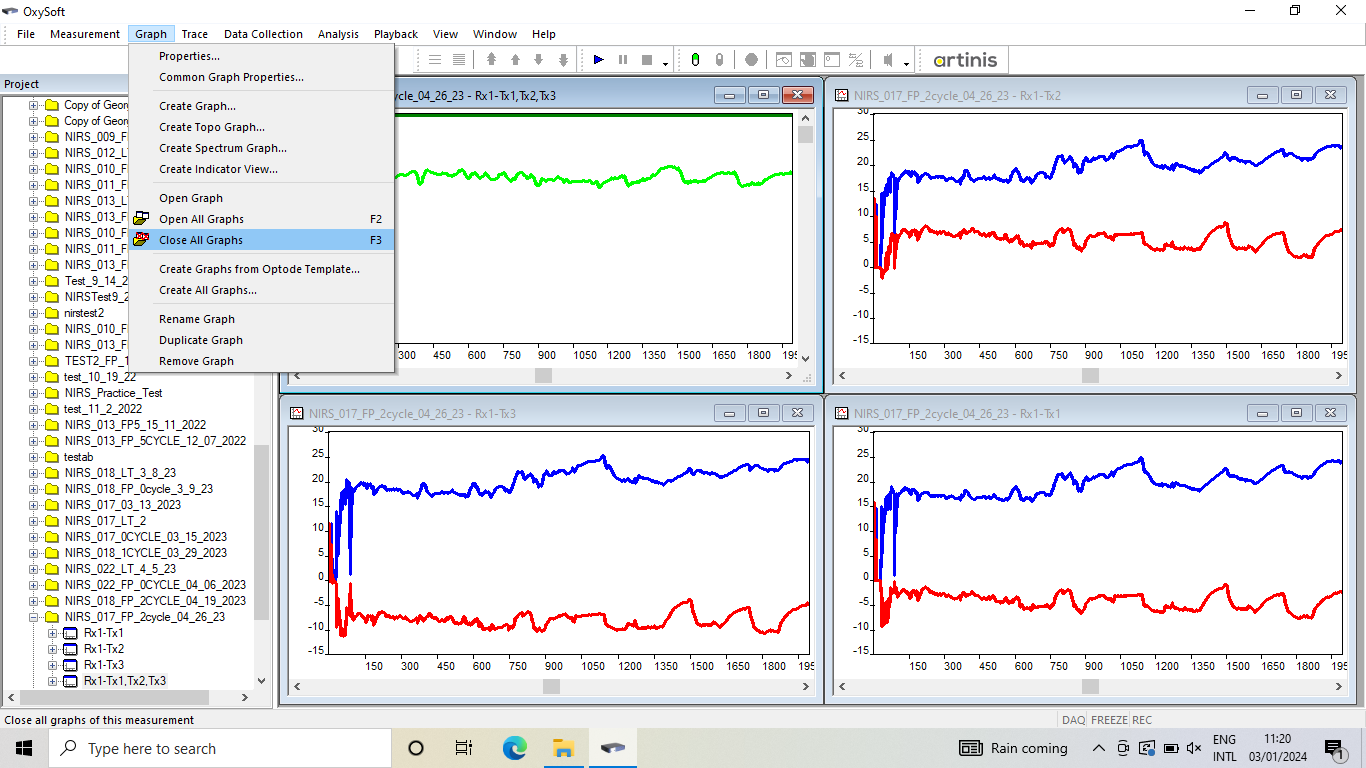
\includegraphics[width=1\linewidth]{images/startnewmeasurement/02_select_close_all_graphs}
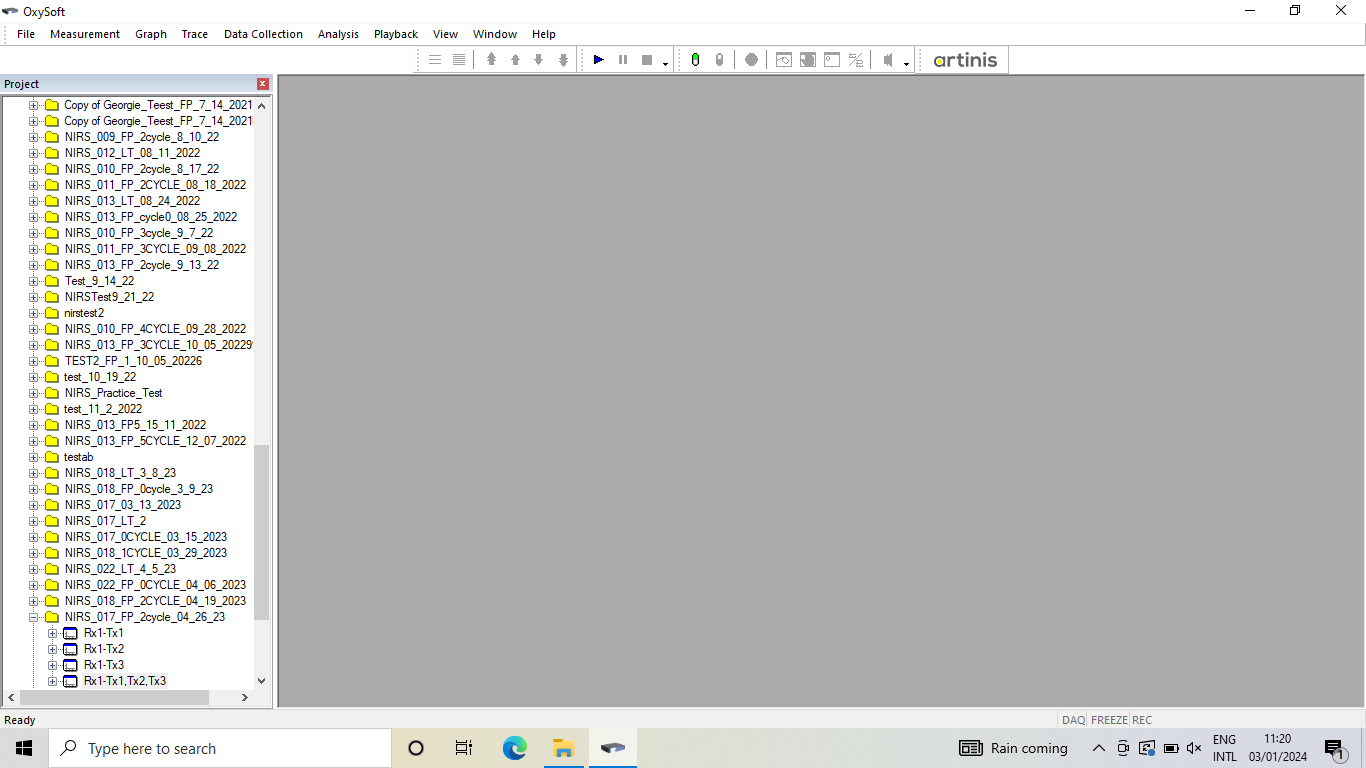
\includegraphics[width=1\linewidth]{images/startnewmeasurement/03_closed_all_graphs}

\begin{itemize}
\tightlist
\item
  Select \texttt{Measurement} in the top bar.
\item
  Select \texttt{Create\ Measurement\ and\ Start\ Device\ (Wizard)...} from drop down.
\end{itemize}

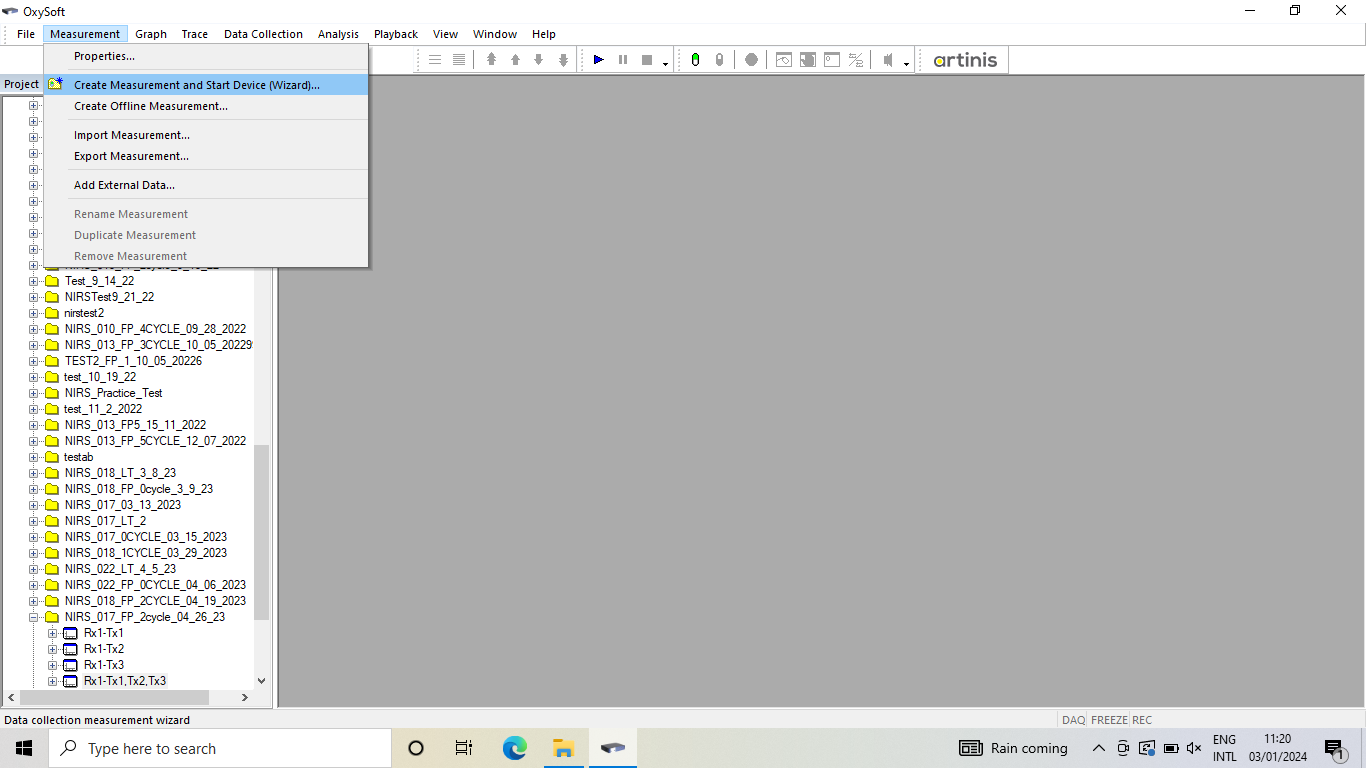
\includegraphics[width=1\linewidth]{images/startnewmeasurement/04_select_start_new}

\begin{itemize}
\tightlist
\item
  Name the measurement appropriately.
\item
  Select the \texttt{Copy\ settings\ from:} drop down.
\item
  Scroll to the top of the drop down and select \texttt{no\ copy}.
\end{itemize}

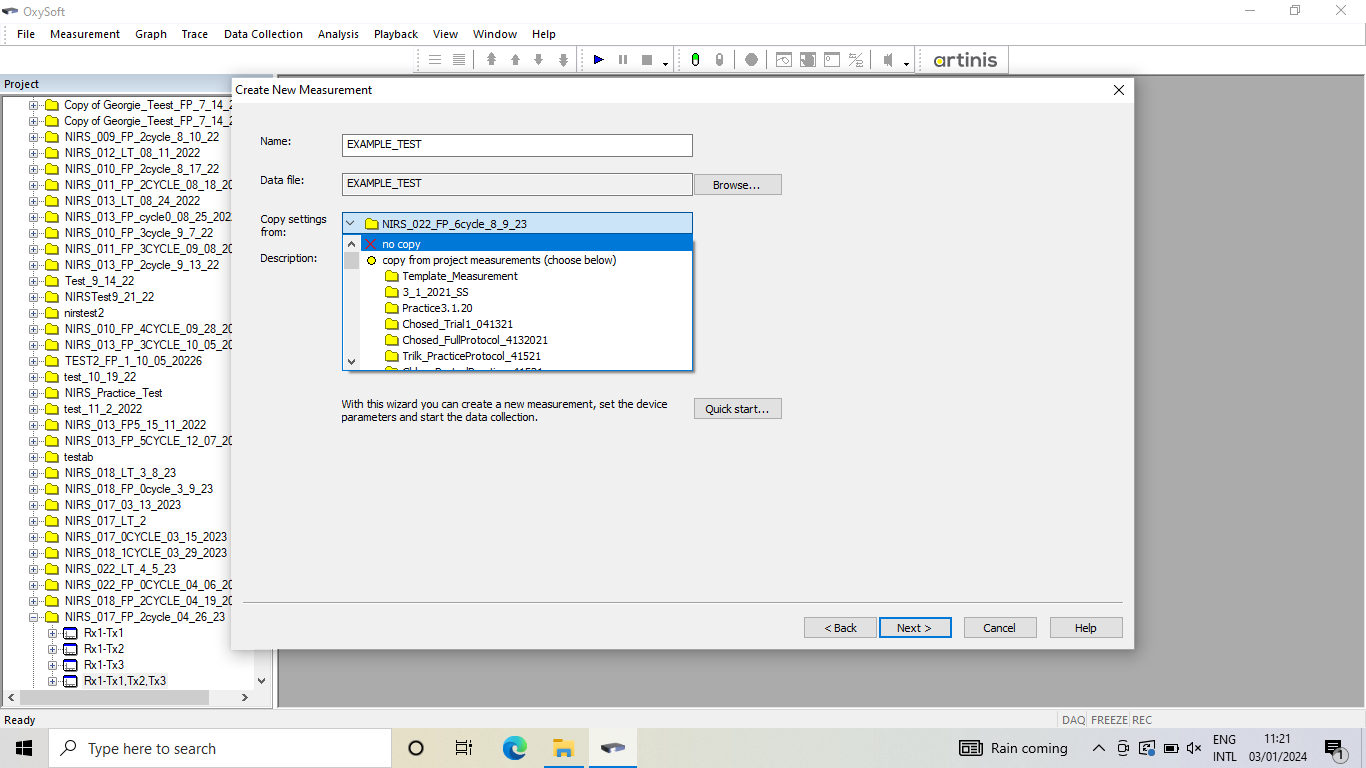
\includegraphics[width=1\linewidth]{images/startnewmeasurement/05_copy_no_settings}

\begin{itemize}
\tightlist
\item
  Click \texttt{Next}. Pop up will open to add a bluetooth device.
\end{itemize}

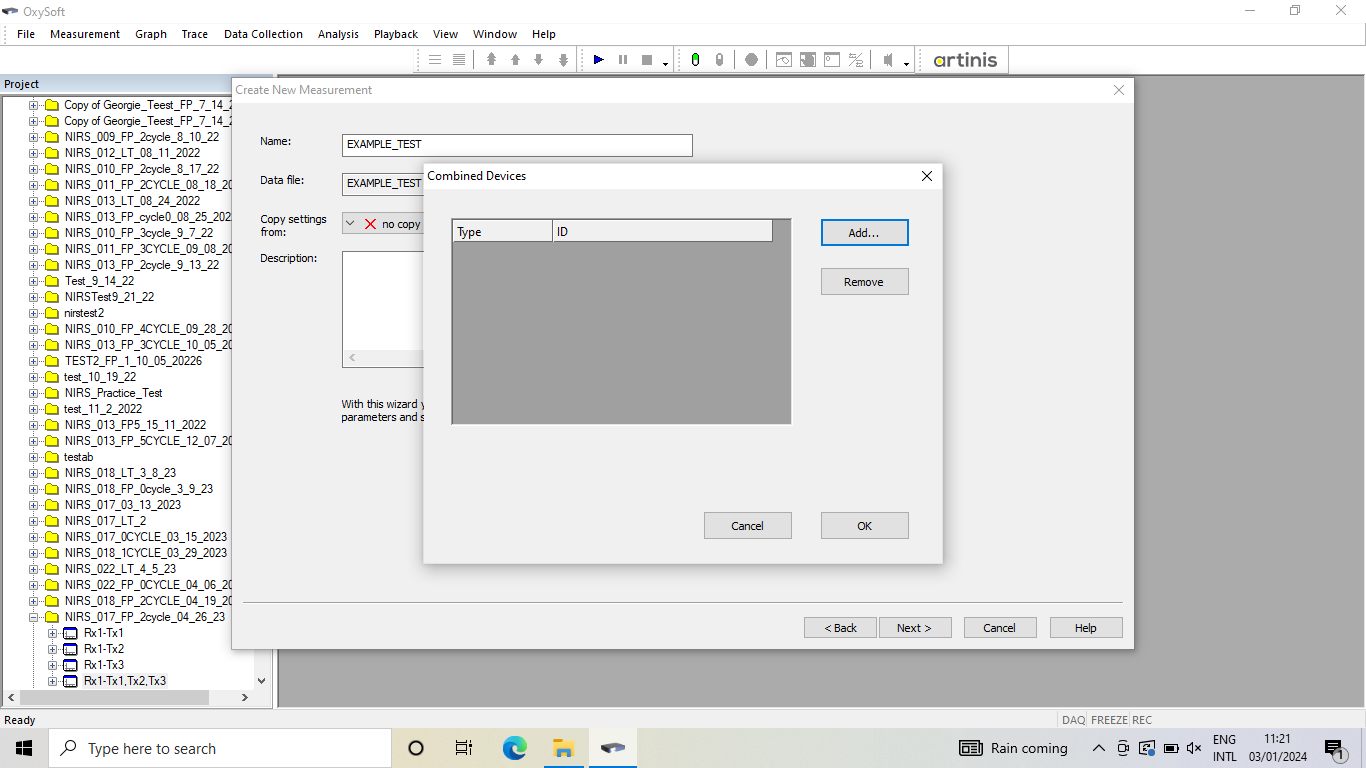
\includegraphics[width=1\linewidth]{images/startnewmeasurement/06_add_device}

\begin{itemize}
\tightlist
\item
  Click \texttt{Add}. Pop up will open to select type of device.
\item
  Select \texttt{OxyMon/PortaMon/PortaLite/OctaMon}, which should be auto filled.
\end{itemize}

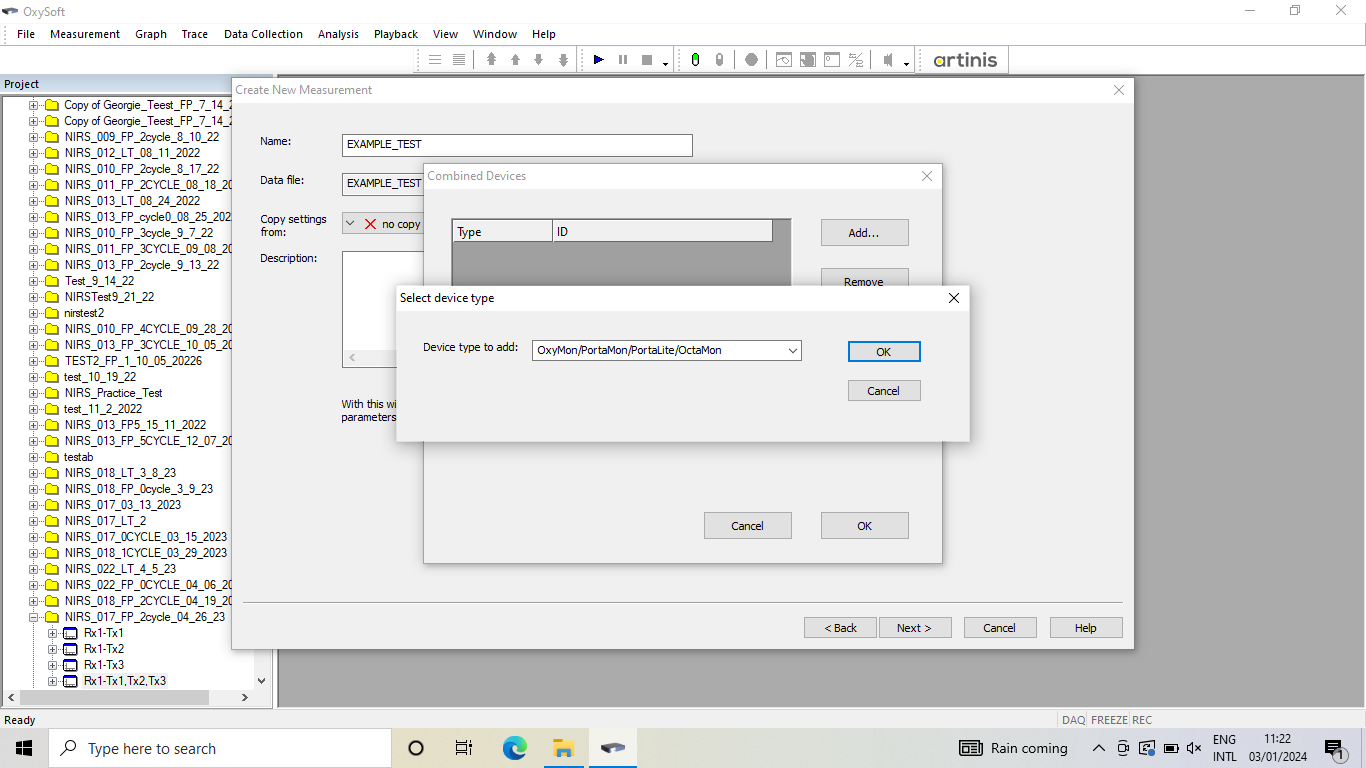
\includegraphics[width=1\linewidth]{images/startnewmeasurement/07_type_of_device_to_add}

\begin{itemize}
\tightlist
\item
  Click \texttt{OK}.
\item
  Select correct device number, this should match the number on the top of the Portamon.
\end{itemize}

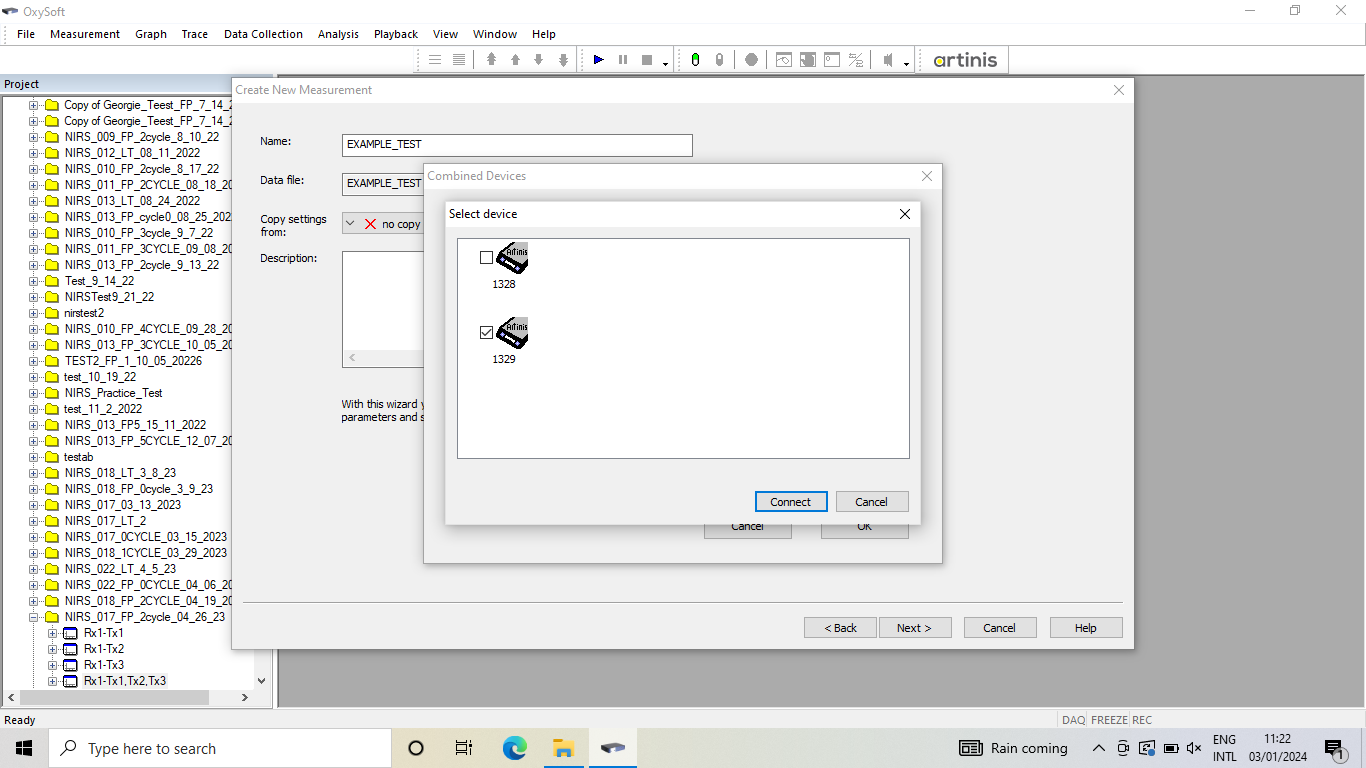
\includegraphics[width=1\linewidth]{images/startnewmeasurement/08_device_number}

\begin{itemize}
\tightlist
\item
  Click \texttt{Connect}.
\item
  Device should pair with the computer. If it does not, try the following steps:

  \begin{itemize}
  \tightlist
  \item
    Check the device is on. The green LED light should be on. If not, turn on by holding down the button on the left until the lights come on (about three seconds).
  \item
    Hold the bluetooth button down for about three seconds while you click \texttt{connect} on the computer.
  \item
    Unpair the device with the computer in the computer's bluetooth settings, then re-pair.
  \item
    Restart the computer.
  \item
    Try using the other Portamon.
  \end{itemize}
\item
  When successfully connected, a blue LED will turn on on the Portamon and the device type and number will be listen in the \texttt{Combined\ Devices} pop up.
\end{itemize}

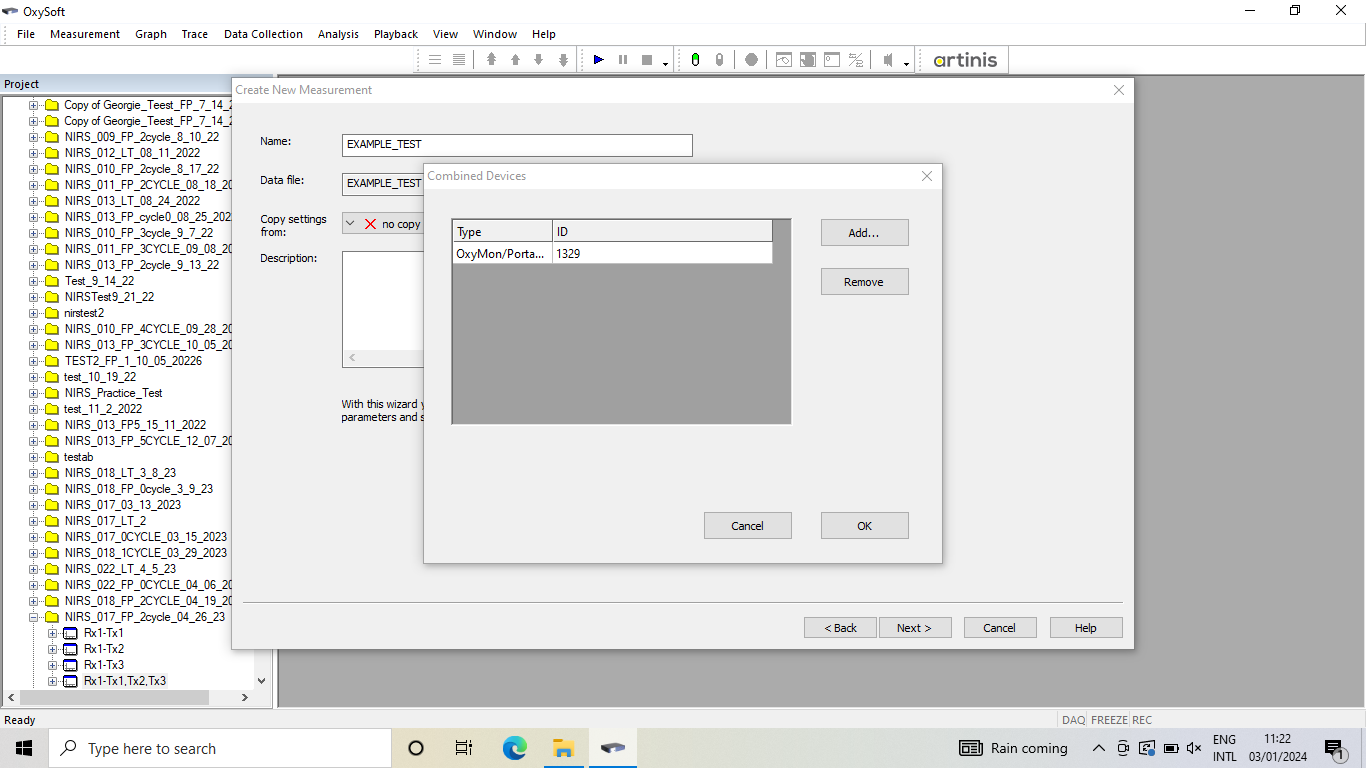
\includegraphics[width=1\linewidth]{images/startnewmeasurement/09_successful_connection}

\begin{itemize}
\tightlist
\item
  Click \texttt{OK}.
\item
  The Optode-template window will now be open.
\item
  Under \texttt{Optode-template:\ (Filtered\ by\ PortaMon)} click the drop down.
\item
  Select \texttt{Portamon\ TSI\ Fit\ Factor}.
\end{itemize}

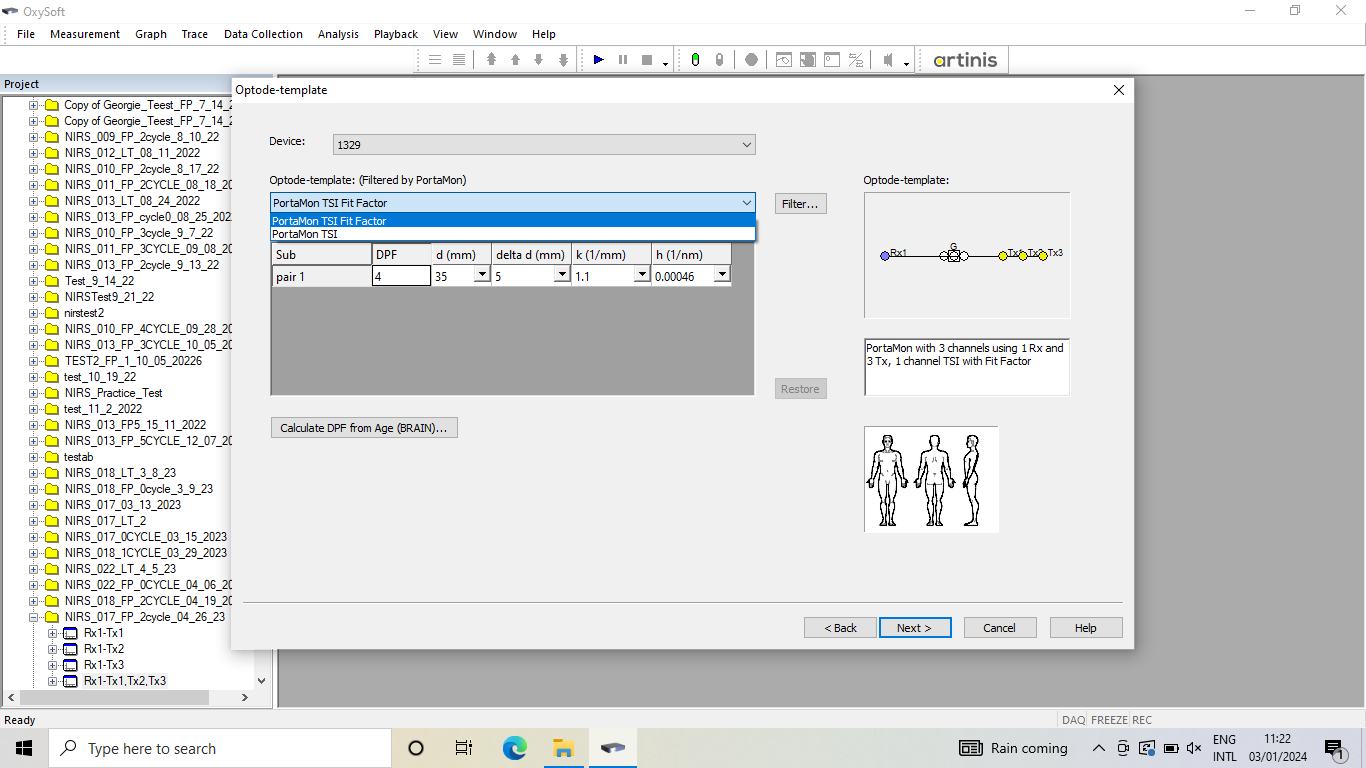
\includegraphics[width=1\linewidth]{images/startnewmeasurement/10_select_tsiff}

\begin{itemize}
\tightlist
\item
  Under \texttt{k\ (1/mm)} click the drop down.
\item
  Select \texttt{1.63\ (calf)}.
\end{itemize}

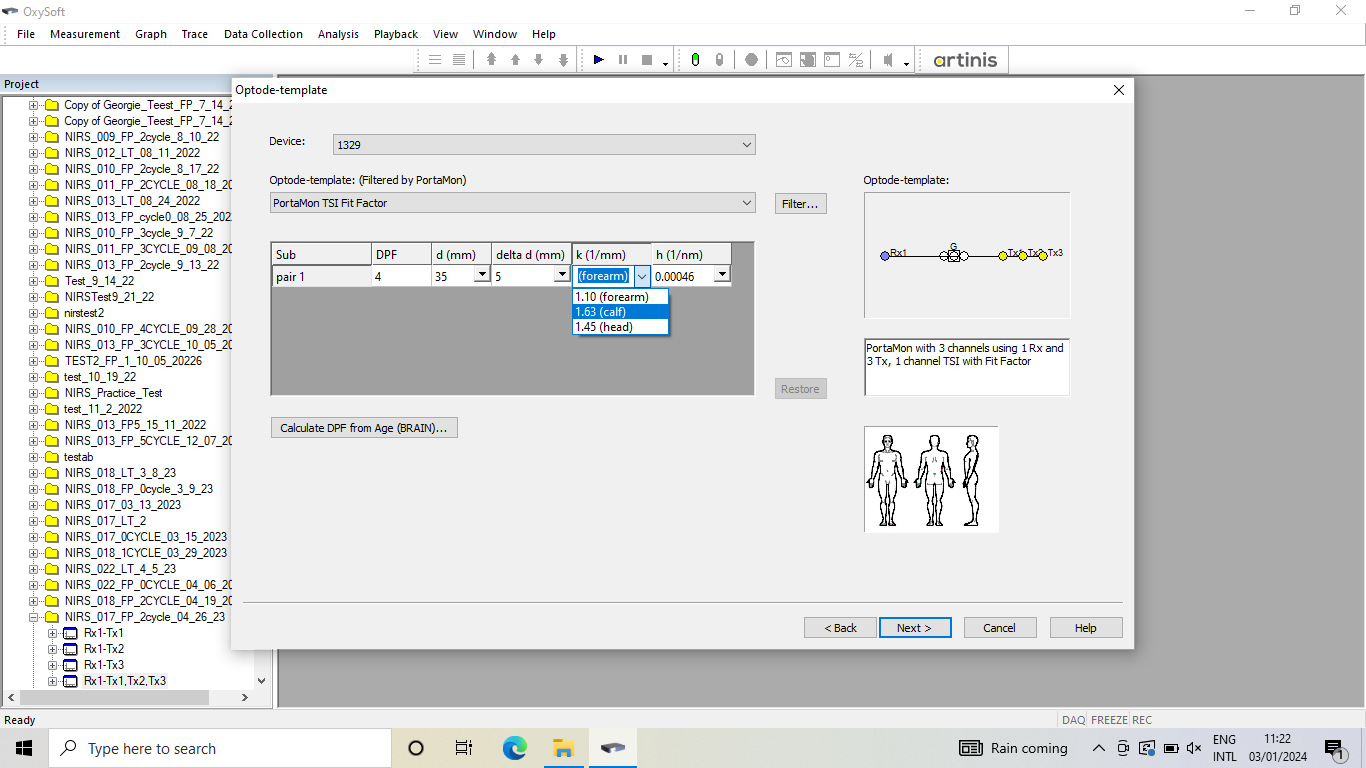
\includegraphics[width=1\linewidth]{images/startnewmeasurement/11_k_calf}

\begin{itemize}
\tightlist
\item
  Under \texttt{h\ (1/mm)} click the drop down.
\item
  Select \texttt{5.5e-4\ (calf)}.
\end{itemize}

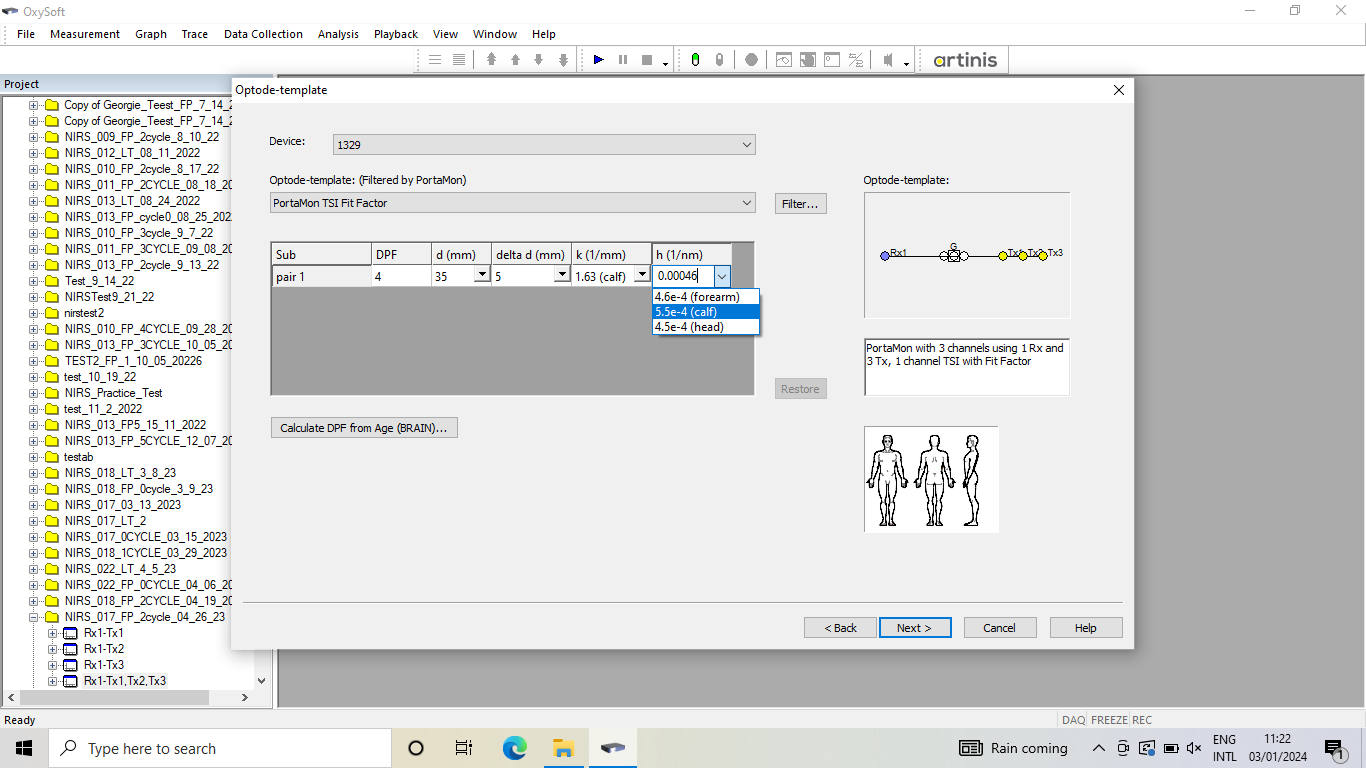
\includegraphics[width=1\linewidth]{images/startnewmeasurement/12_h_calf}

\begin{itemize}
\tightlist
\item
  Click \texttt{Next}.
\item
  The Light Source to Optode Mapping window will now be open. Leave all settings as is and click \texttt{Next}.
\end{itemize}

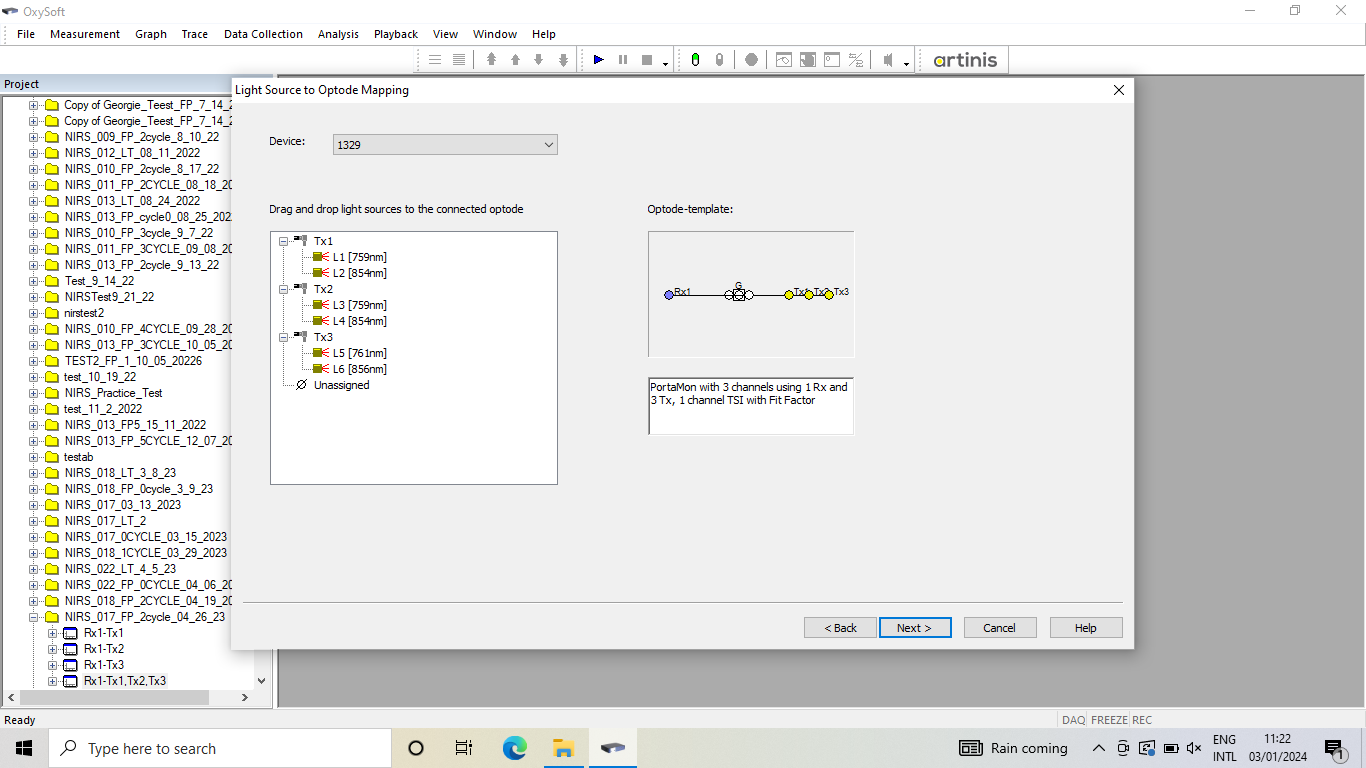
\includegraphics[width=1\linewidth]{images/startnewmeasurement/13_optodemapping_popup}

\begin{itemize}
\tightlist
\item
  The Device settings window will now be open. Leave all settings as is and click \texttt{Next}.
\end{itemize}

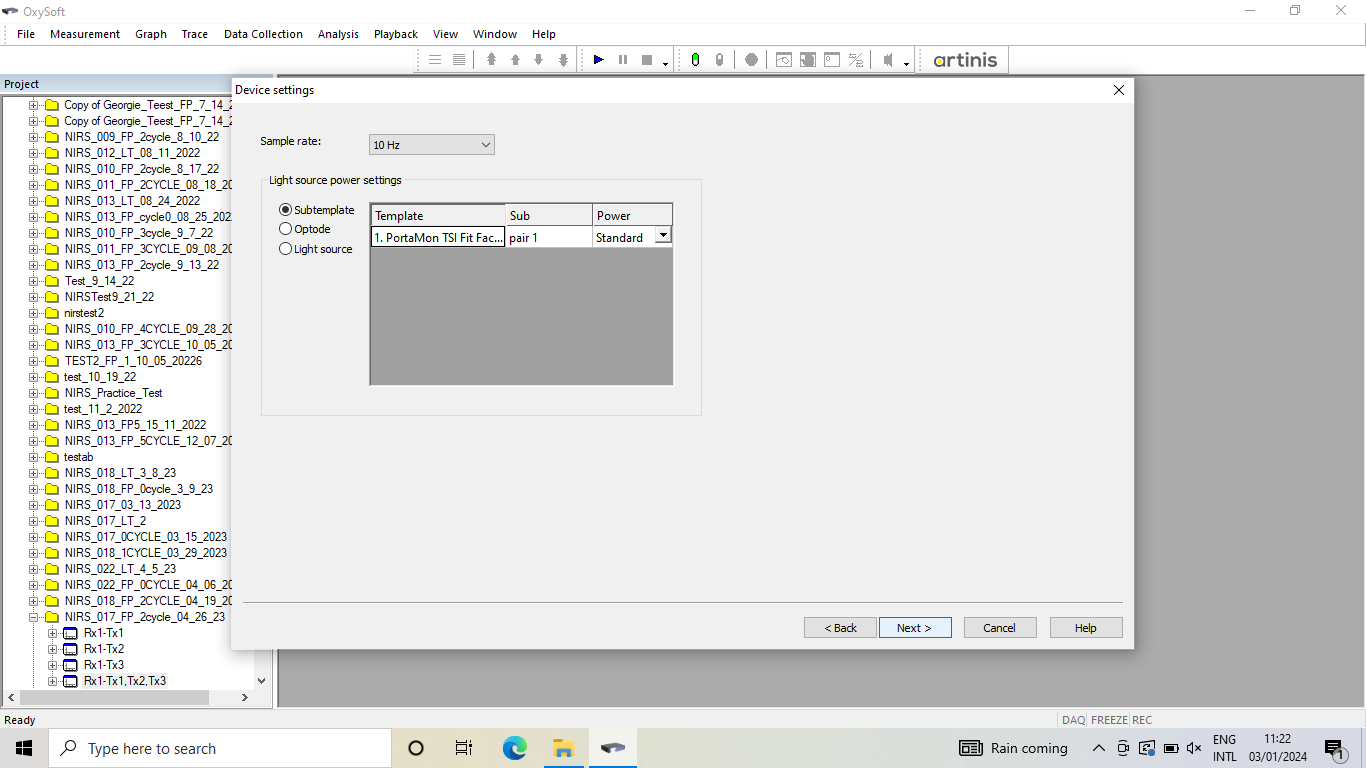
\includegraphics[width=1\linewidth]{images/startnewmeasurement/14_device_settings_popup}

\begin{itemize}
\tightlist
\item
  The Further Options window will now be open. The \texttt{Action} drop down should have \texttt{Start\ measurement\ after\ finishing\ wizard} selected.
\end{itemize}

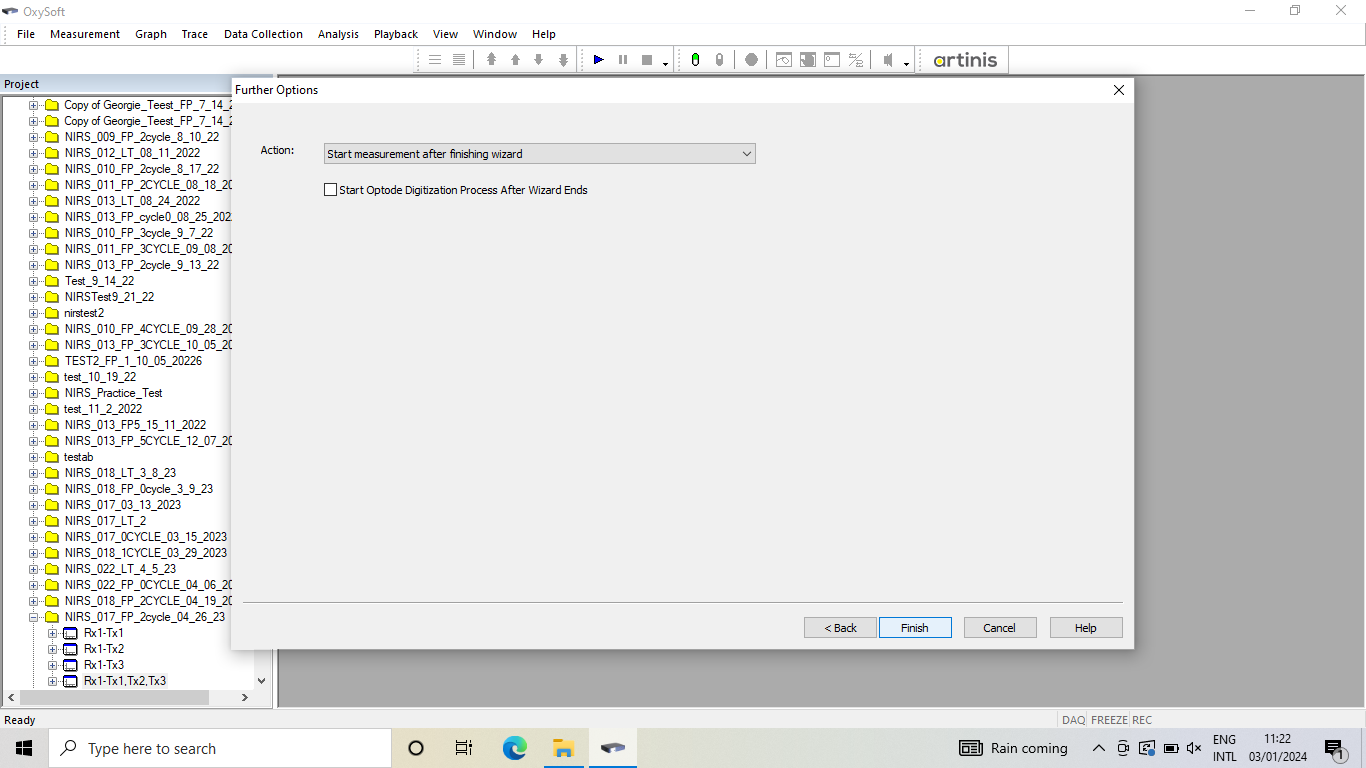
\includegraphics[width=1\linewidth]{images/startnewmeasurement/15_furtheroptions_popup}

\begin{itemize}
\tightlist
\item
  Click \texttt{Finish}.
\item
  The Create All Graphs window will pop up. Leave settings as is and click \texttt{OK}.
\end{itemize}

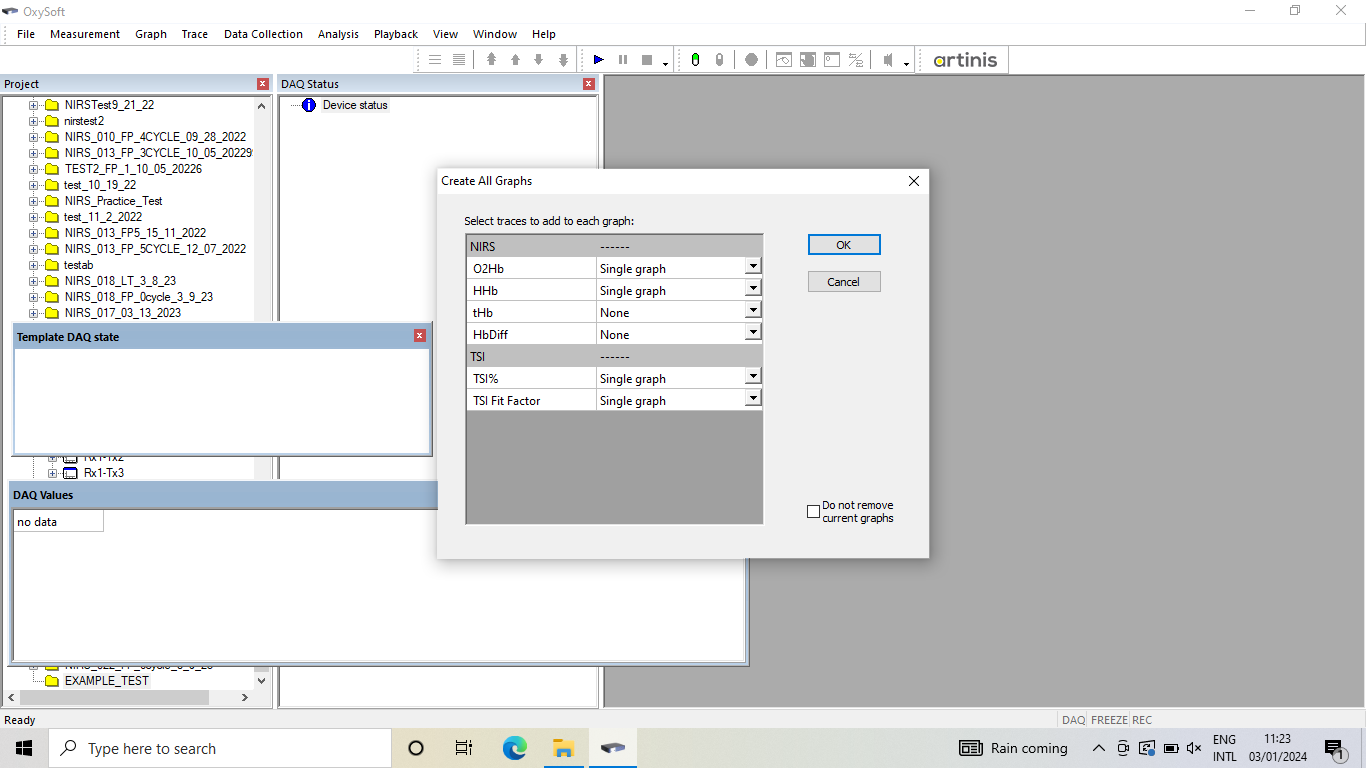
\includegraphics[width=1\linewidth]{images/startnewmeasurement/16_create_all_graphs_popup}

\begin{itemize}
\tightlist
\item
  There will be an Oxysoft pop up. It says `The program will enable the light sources now. Are you sure you want to start the device(s)?' DO NOT click yes yet. Wait until device has been placed correctly. Follow the steps described in \ref{PortaMon-Placement}.
\end{itemize}

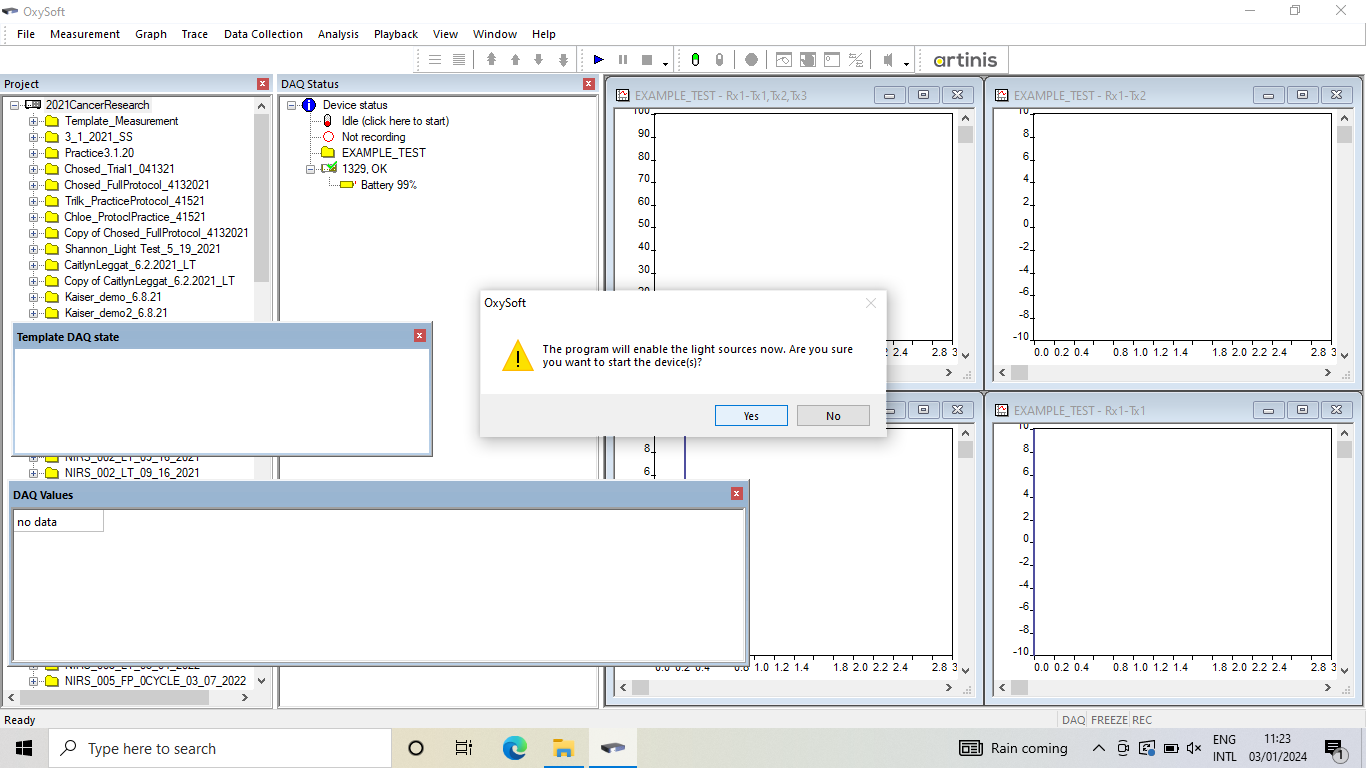
\includegraphics[width=1\linewidth]{images/startnewmeasurement/17_enable_light_sources_popup}

\hypertarget{PortaMon-Placement}{%
\subsection{Instrument Placement on Vastus Lateralis}\label{PortaMon-Placement}}

The PortaMon can measure up to 2 centimeters depth into tissue. Since we are interested in muscle oxygenation, the muscle belly has to be within 2 centimeters from the surface of the skin. Otherwise, the device is not measuring muscle oxygenation but adipose tissue oxygenation. Therefore, we use an ultrasound to measure the subcutaneous adipose tissue thickness.

Place the device over the location measured by ultrasound.

Connect the NIRS by following the steps under \ref{PortaMon-StartMeasurement}.

Click `yes' to enable light sources and begin data collection. Wait approximately 10 seconds. Check the DAQ (Data Acquisition) values to determine whether the NIRS is receiving good data. If one or more of the DAQ values show as red, then make small adjustments to the placement of the device to attempt to get better DAQ values. If the small adjustments add up to a large difference from the original ultrasound measurement location, re-measure adipose tissue thickness using the ultrasound in the new location.

When all three DAQ values remain white when the subject moves around their leg, then the device is in the best location. If one of the DAQ values turns red during movement, that can be okay but only ONE. If two of the DAQ values are red, then TSI cannot be calculated so we do our best to have at least two good signals, three if at all possible.

Rock the device laterally and remove the tape cover on the exposed side. Rock the device back into place and stick the tape to the subject's skin. Repeat on the other side. Double check that the DAQ values remain consistent.

Take a picture of the placement. Use a measuring tape to show the distance from the top of the kneecap to the bottom of the device and use a perpendicular measuring tape to show the distance from the center of the thigh to the right edge of the device. Print the picture and place in the participant's physical file. Upload a .png of the picture into the RedCap.

\hypertarget{PortaMon-DataCollection}{%
\section{During Data Collection}\label{PortaMon-DataCollection}}

\begin{itemize}
\tightlist
\item
  When the device is placed correctly, click yes. The new measurement will begin.
\end{itemize}

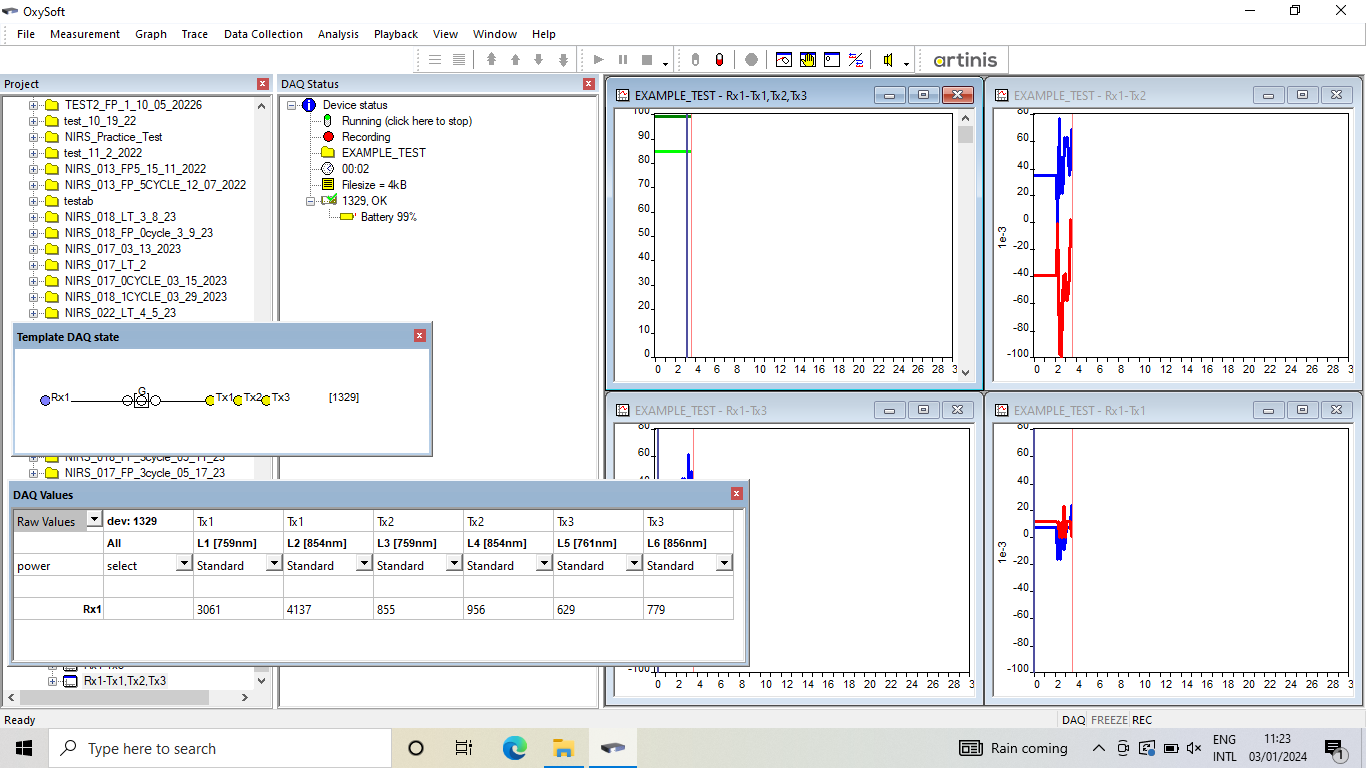
\includegraphics[width=1\linewidth]{images/startnewmeasurement/new_measurement_begins}

\begin{itemize}
\tightlist
\item
  When you are done with the measurement, click the red pill in the top bar to stop the light sources. Oxysoft will stop the rolling every 30 seconds view and you will be able to see the whole measurement in the panes.
\end{itemize}

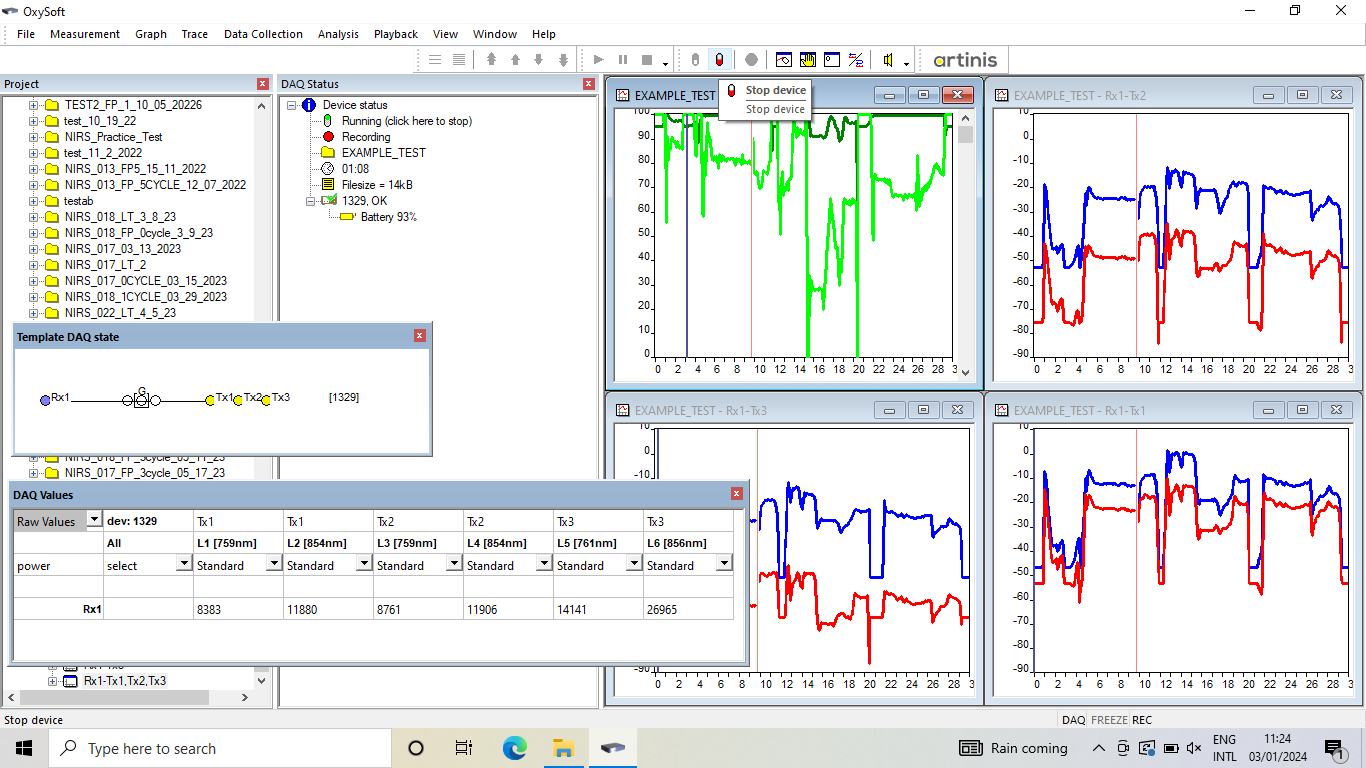
\includegraphics[width=1\linewidth]{images/startnewmeasurement/select_end_measurement}
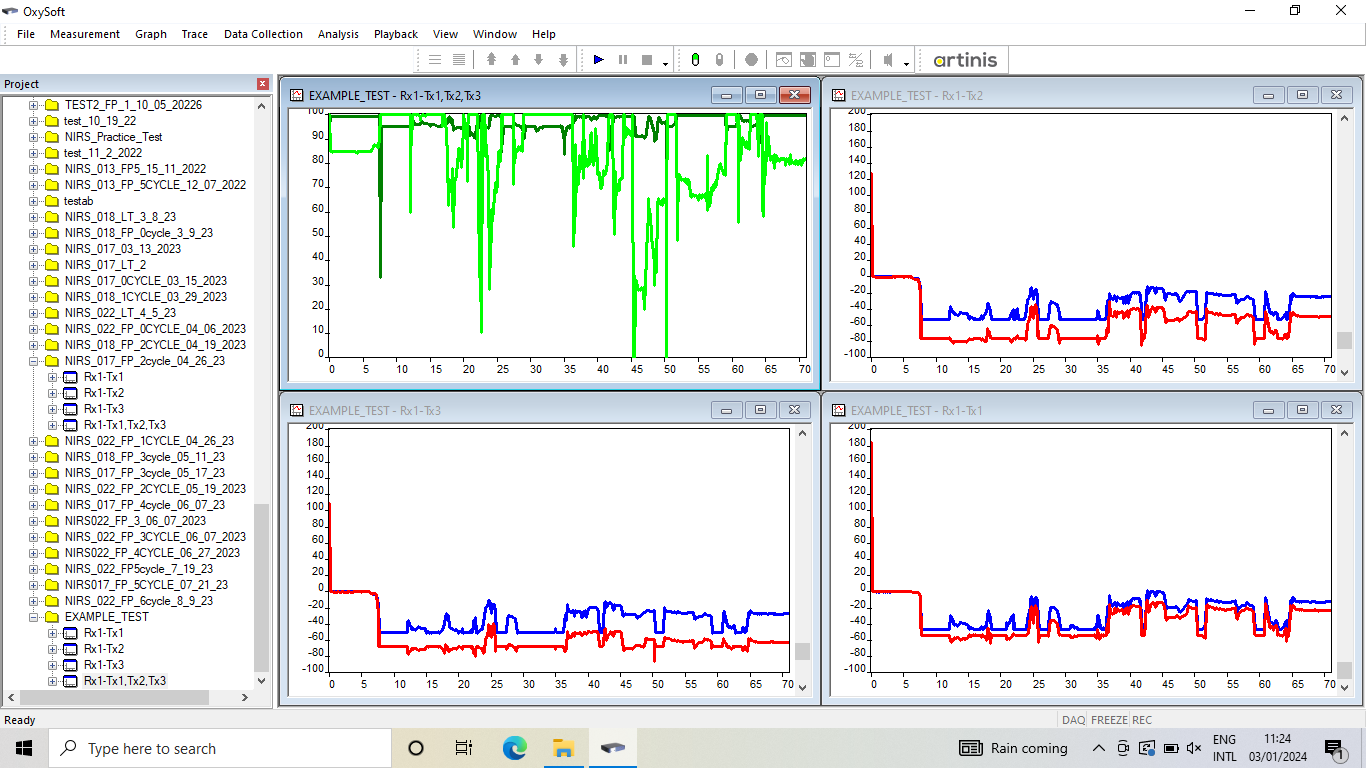
\includegraphics[width=1\linewidth]{images/startnewmeasurement/view_whole_measurement}

\hypertarget{PortaMon-AfterDataCollection}{%
\section{After Data Collection}\label{PortaMon-AfterDataCollection}}

\hypertarget{PortaMon-ChangeProperties}{%
\subsection{Change Measurement Properties}\label{PortaMon-ChangeProperties}}

\begin{itemize}
\tightlist
\item
  Right click on the name of the measurement in the \texttt{Project} panel on the left.
\item
  Select \texttt{Properties...}. This will open up a new panel.
\end{itemize}

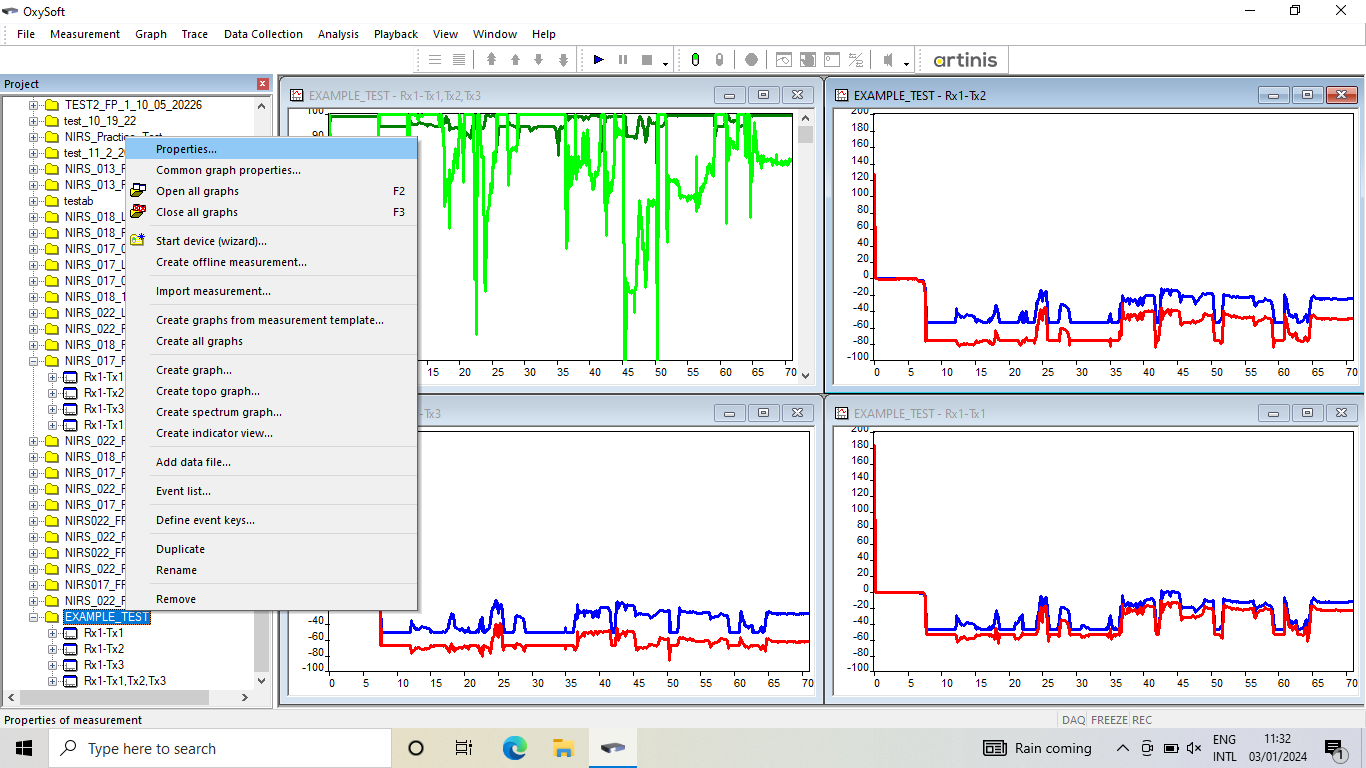
\includegraphics[width=1\linewidth]{images/changemeasurementproperties/select_measurement_properties}
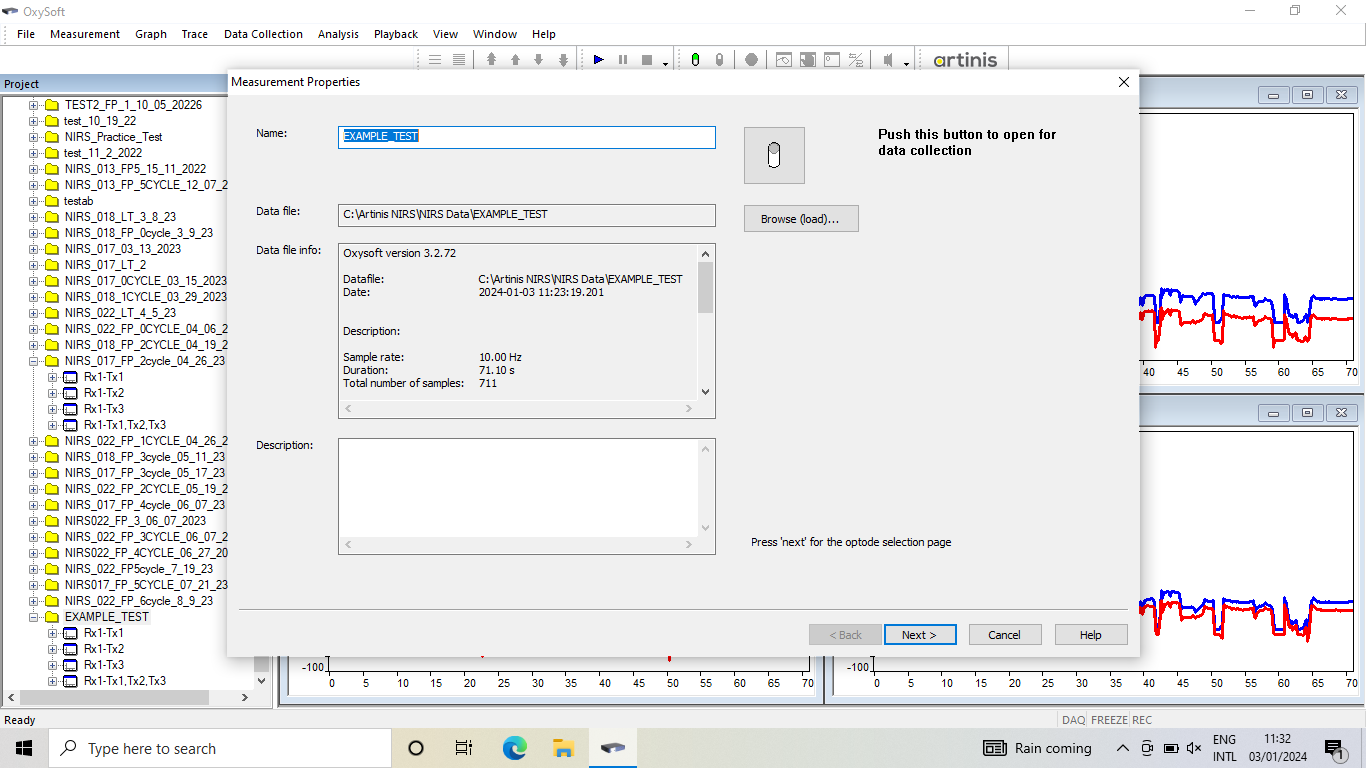
\includegraphics[width=1\linewidth]{images/changemeasurementproperties/opened_measurement_properties}

\begin{itemize}
\tightlist
\item
  Leave the measurement name and data file as is.
\item
  Click \texttt{Next}.
\item
  Under \texttt{Optode\ -template:} select \texttt{PortaMon\ TSI} instead of \texttt{PortaMon\ TSI\ Fit\ Factor}.
\end{itemize}

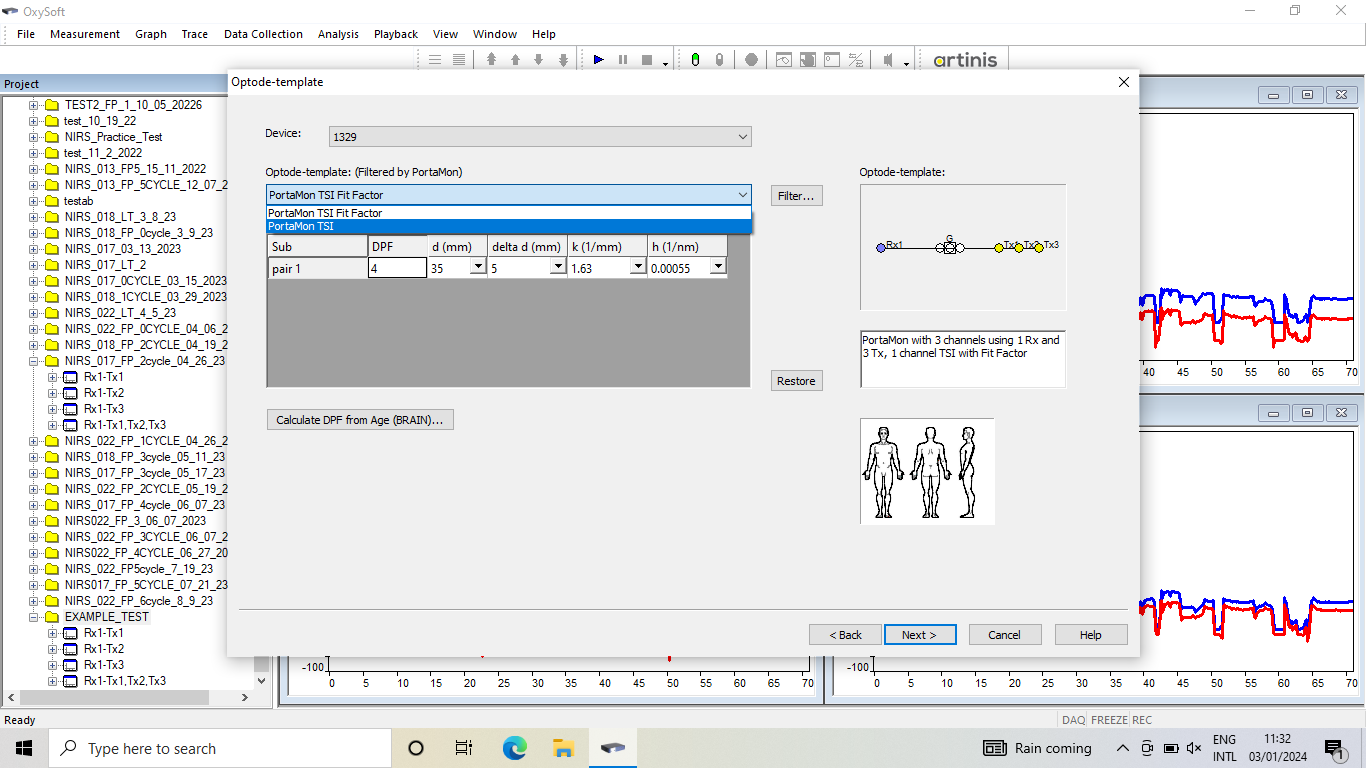
\includegraphics[width=1\linewidth]{images/changemeasurementproperties/select_tsi}

\begin{itemize}
\tightlist
\item
  Change the settings as follows:

  \begin{itemize}
  \tightlist
  \item
    Under \texttt{d\ (mm)} type \texttt{32.5}.
  \item
    Under \texttt{delta\ d\ (mm)} type \texttt{5}.
  \item
    Ensure \texttt{k\ (1/mm)} is \texttt{1.63\ (calf)}. and \texttt{h\ (1/mm)} is \texttt{5e-4\ (calf)}.
  \end{itemize}
\end{itemize}

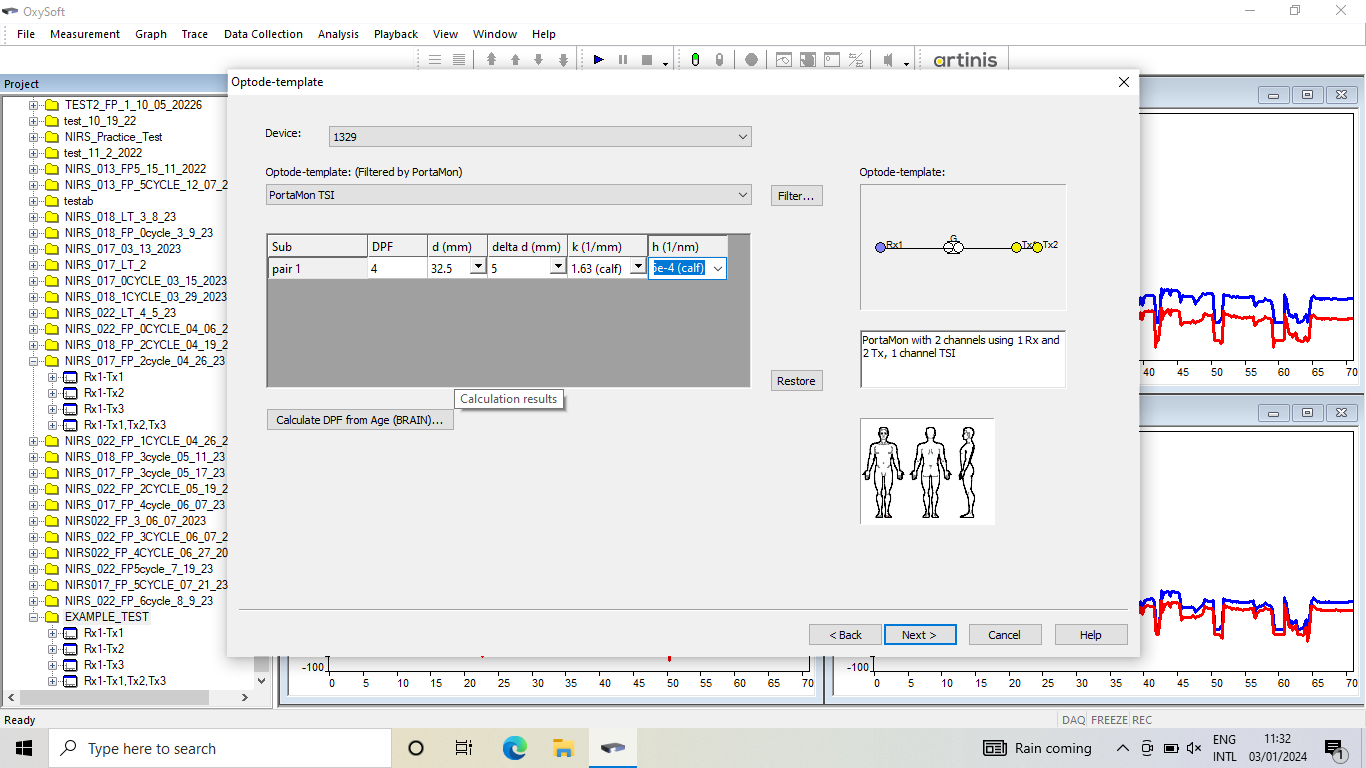
\includegraphics[width=1\linewidth]{images/changemeasurementproperties/tsi_template_settings}

\begin{itemize}
\tightlist
\item
  Click \texttt{Next}.
\item
  When \texttt{Tx3} has been removed from the TSI calculations, the graph panels will look different. The \texttt{Rx1-Tx3} panel will have two flat lines, one blue and one red. The \texttt{TSIFF} panel will still have a green line for \texttt{TSI}, and will no longer have a \texttt{TSIFF} line in that panel.
\end{itemize}

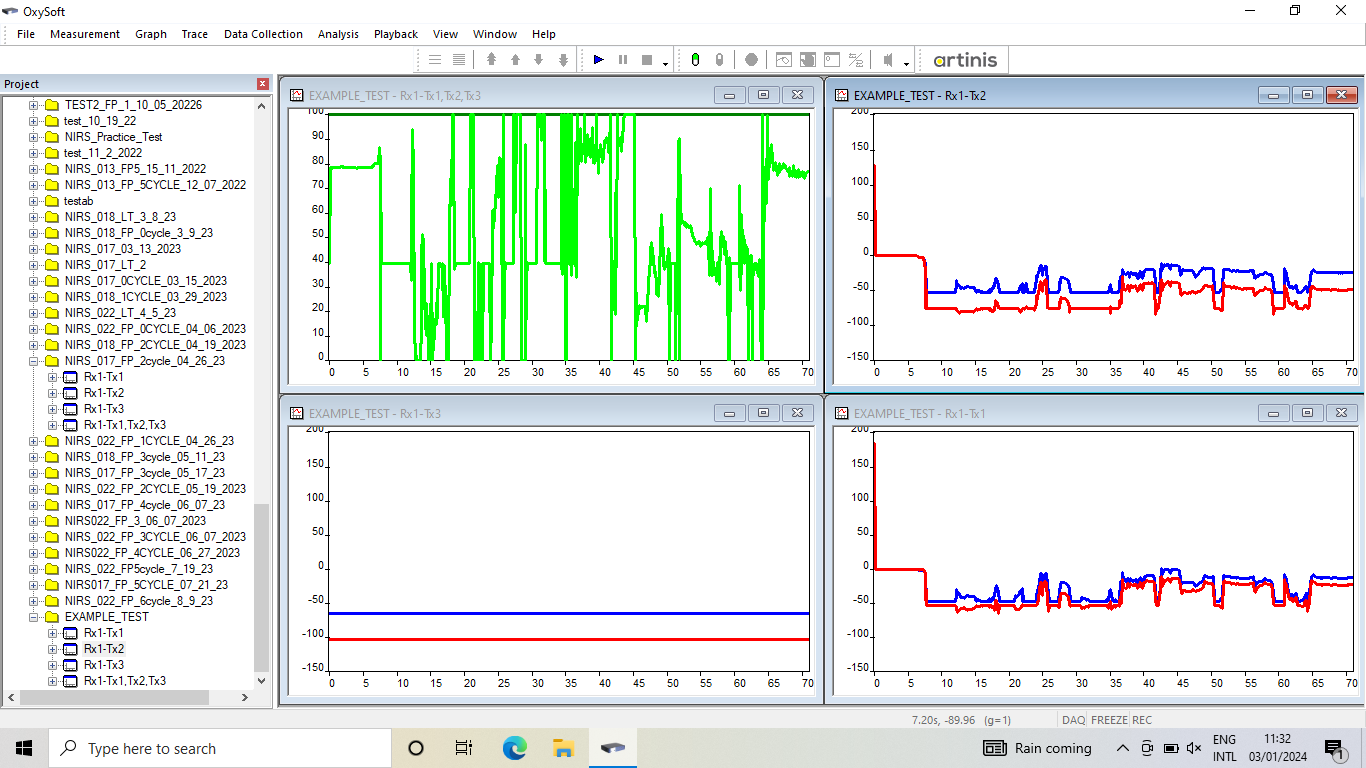
\includegraphics[width=1\linewidth]{images/changemeasurementproperties/view_tsi_graphs}

To undo these changes and revert to the original measurement with \texttt{Tx3} included in the \texttt{TSI} calculations, right click on the file name and open up the \texttt{Properties} panel again. Click \texttt{Next}.

Next to the \texttt{Optode-template} settings table, there is a button on the bottom right that says \texttt{Restore}. Click \texttt{Restore}. Click \texttt{Next}.

The graphs are now restored to their original state.

\hypertarget{PortaMon-DataExport}{%
\subsection{Data Export}\label{PortaMon-DataExport}}

Ensure that only one measurement is open in the Oxysoft graph panels. Do this by closing all graphs, then selecting the name of the measurement you want to open in the file pane on the left.

If you are not sure or cannot tell, under the \texttt{Graph} drop down of the header bar, select \texttt{Close\ all\ graphs}. There should be no visible graphs in the main panel.

Select the name of the measurement you want to export in the \texttt{Project} panel on the left. Click \texttt{Open\ all\ graphs} under the \texttt{Measurement} drop down while the name of the file is highlighted. There should be four panels open, one titled \texttt{Tx1-Rx1}, \texttt{Tx2-Rx1}, \texttt{Tx3-Rx1}, and one \texttt{TSIFF}.

If all three transmitters had good DAQ values during data collection and never dropped into red, skip the next steps. If there were issues with only Tx3, follow the steps described in \ref{Appendix-Instruments-PortaMon-Usage-ChangeProperties}.

Select \texttt{Export\ measurement} under the \texttt{Measurement} dropdown.

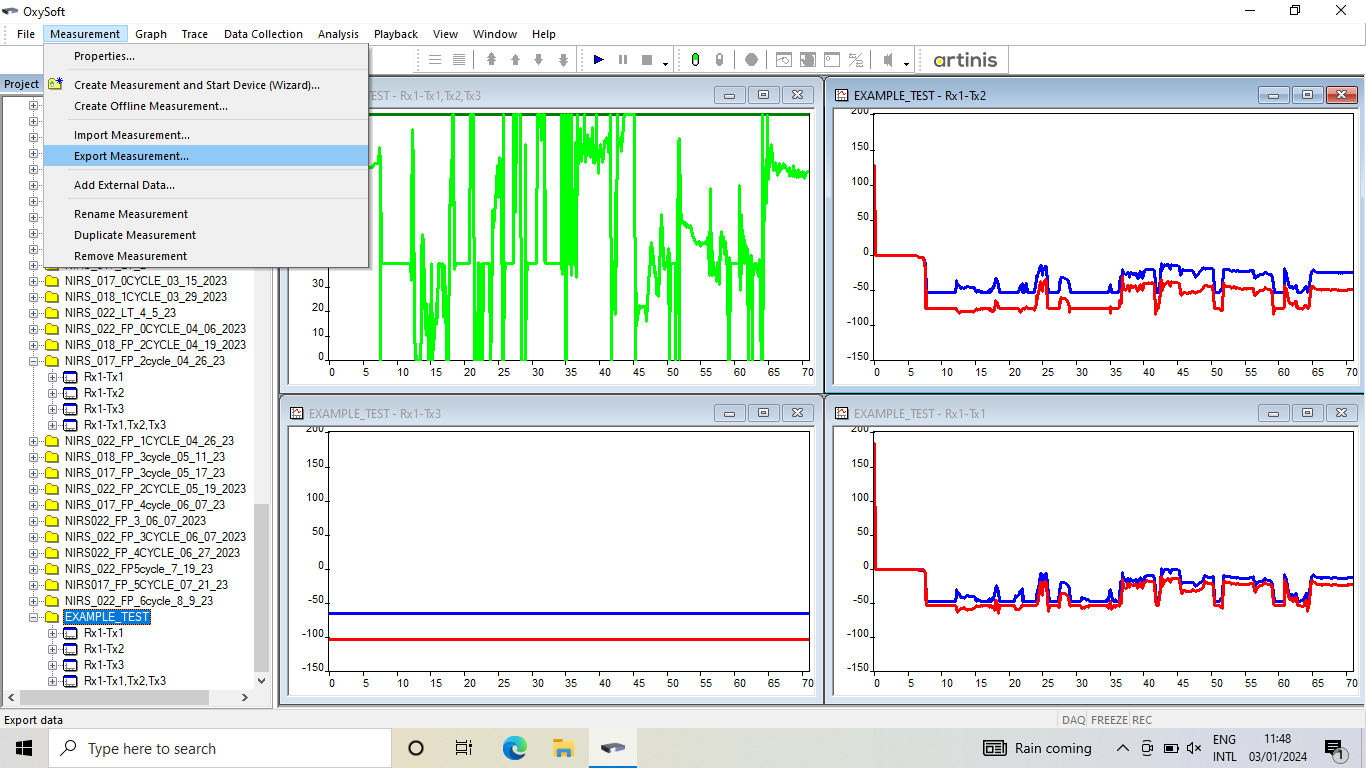
\includegraphics[width=1\linewidth]{images/exportmeasurement/1_selectmeasurementtoexport}

A new panel will open. Select the type of file you wish to export as. The automatic selection is text (\texttt{.txt}), which is the preferred type of export.

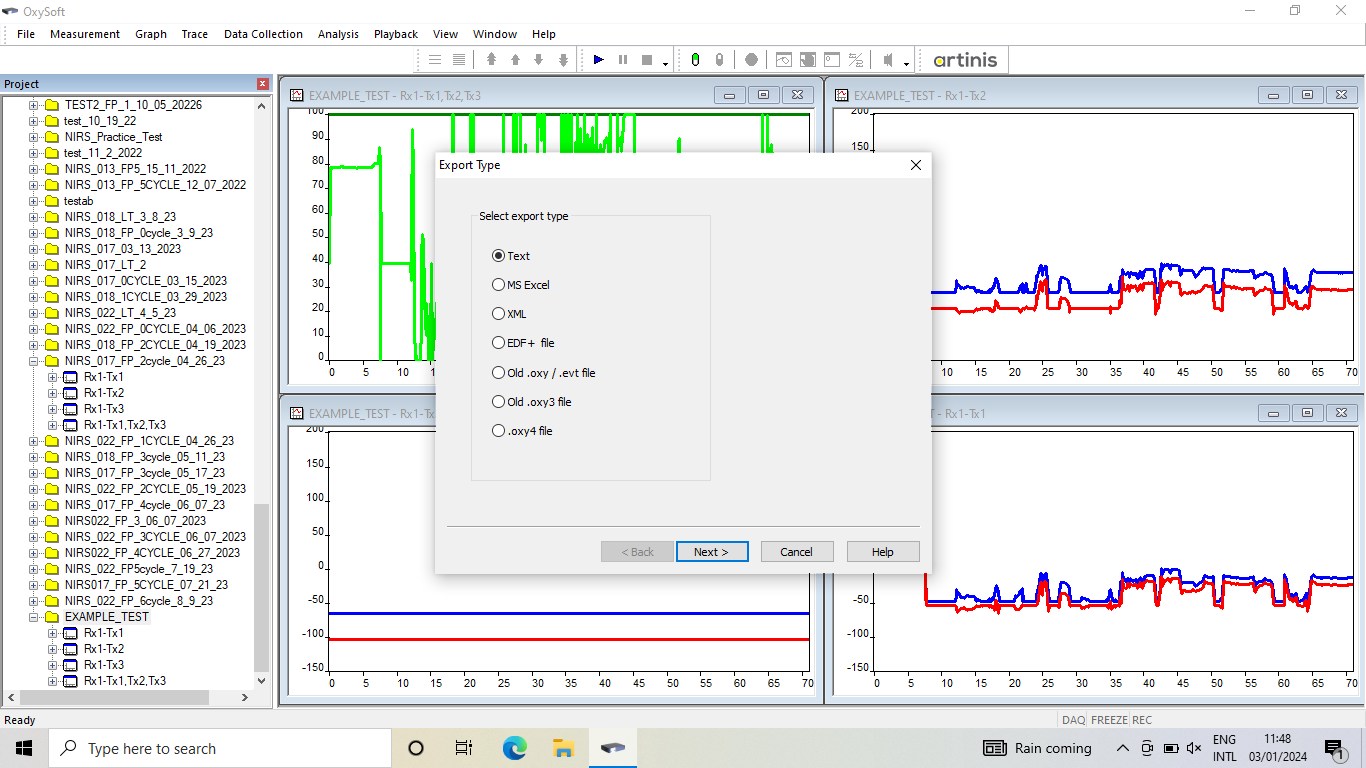
\includegraphics[width=1\linewidth]{images/exportmeasurement/2_selecttypeofexport}

Click \texttt{Next}.

A new popup will prompt you to choose a location for the exported file.

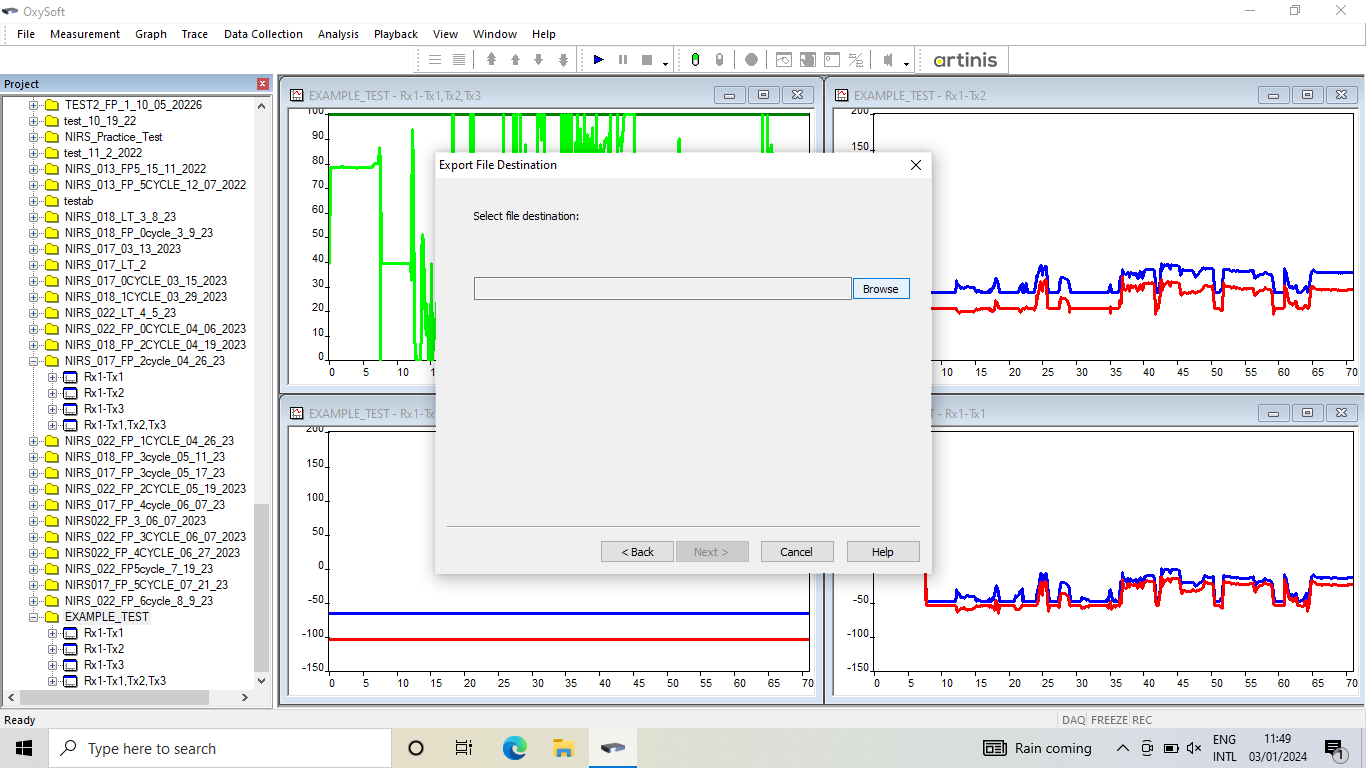
\includegraphics[width=1\linewidth]{images/exportmeasurement/3_choosefilelocation}

Click \texttt{Browse}.

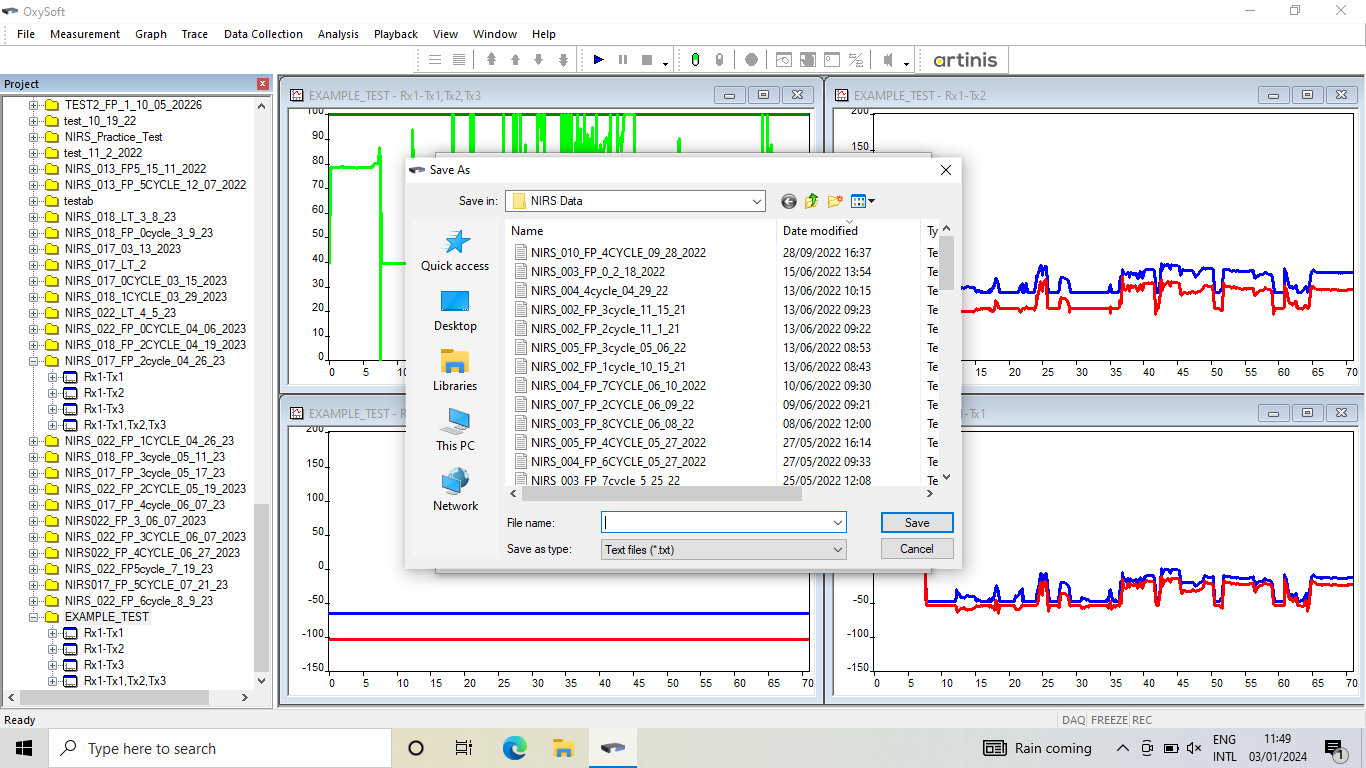
\includegraphics[width=1\linewidth]{images/exportmeasurement/4_filelocationpopup}

There is a folder on the desktop for all data for the NIRS study. Select that folder as the destination. In the file name bar, type in the name of the measurement. I prefer for the exported file and the name of the measurement in Oxysoft to match for consistency. When you type in the name of the measurement in oxysoft, it will prompt you to select \texttt{nameofthefile.oxy4}. Do not select this. Just type the name of the measurement with no file extension.

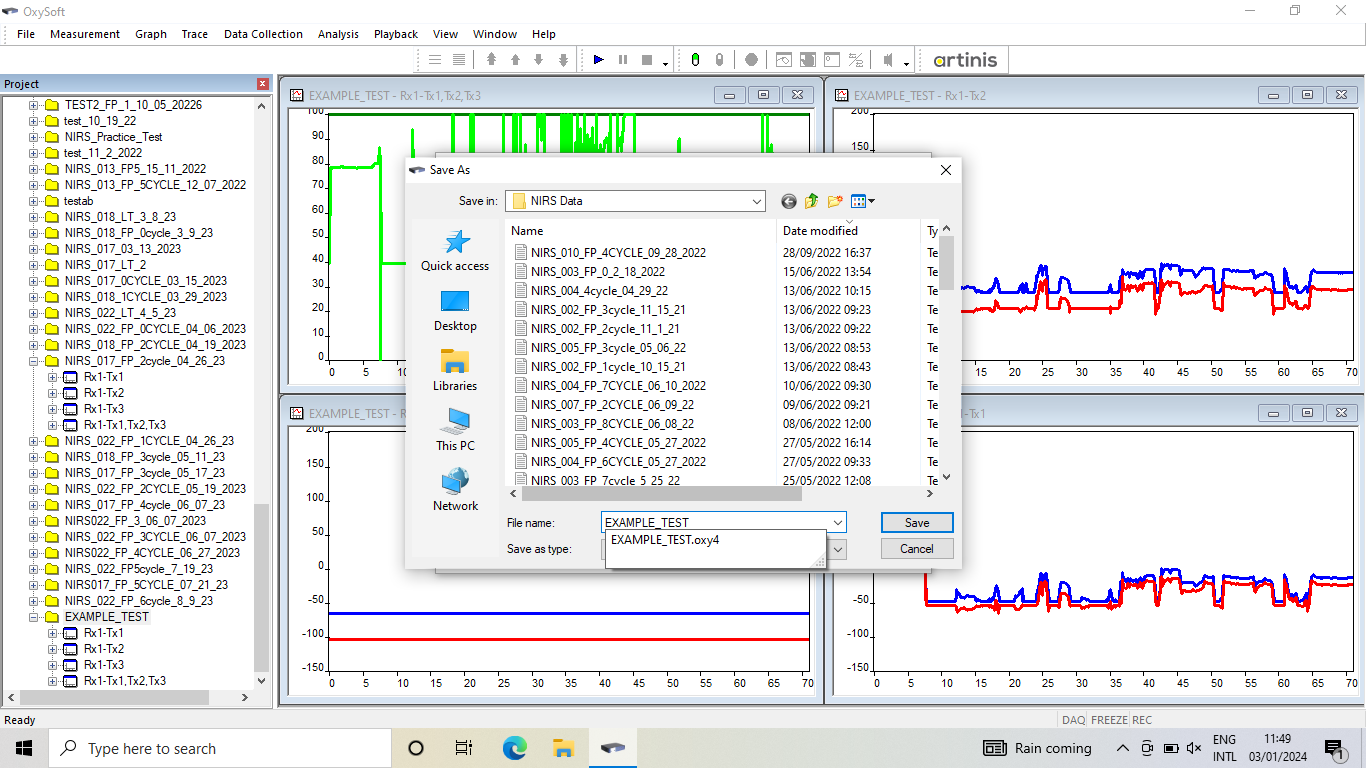
\includegraphics[width=1\linewidth]{images/exportmeasurement/5_nameexportfile}

Click \texttt{Save}.

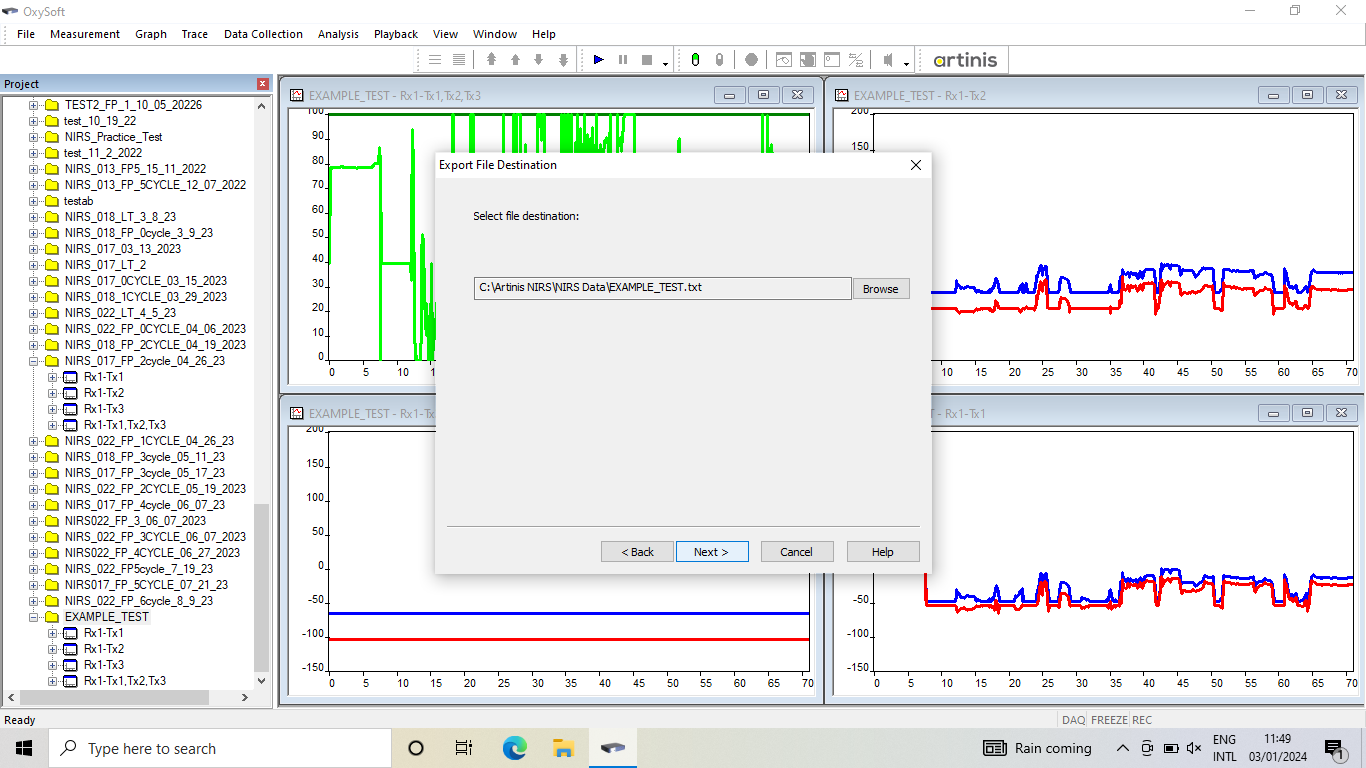
\includegraphics[width=1\linewidth]{images/exportmeasurement/6_chosenfilelocation}

The file path should be to the NIRS data folder and should be named the same as the measurement with a \texttt{.txt} extension.

Click \texttt{Next}.

The \texttt{Export\ Options} popup will have several selections for the type of data to export. Leave the default selection, \texttt{Graph\ data\ of\ open\ graphs}. Click \texttt{Next}.

\includegraphics[width=1\linewidth]{images/exportmeasurement/7_chooseexportopengraphs}

The \texttt{Export\ Time\ Span} pop up will have the option to remove data from the beginning or end of the measurement. Leave the time span as it is and export the full measurement. Click \texttt{Start\ Export}.

\includegraphics[width=1\linewidth]{images/exportmeasurement/8_exportwholemeasurement}

\hypertarget{Parvo}{%
\chapter{ParvoMedics TrueOne 2400}\label{Parvo}}

\hypertarget{Parvo-Specs}{%
\section{Specifications}\label{Parvo-Specs}}

The \href{http://www.parvo.com/}{TrueOne} Metabolic Cart by ParvoMedics measures maximal O2 consumption, indirect calorimetry, and other metabolic conditions.

The computer that has the ParvoMedics software installed is not connected to the internet in any way. It has Windows 7. \textbf{Never connect this computer to the internet or update Windows.} This would require attaining approval to install the ParvoMedics software on PrismaHealth computers, which would take several months. The ParvoMedics software is not frequently updated and Windows updates could break the installation. Everything works as it is, and if it ain't broke, don't fix it.

\hypertarget{Parvo-Software}{%
\section{Software}\label{Parvo-Software}}

\hypertarget{Parvo-BeforeDataCollection}{%
\section{Before Data Collection}\label{Parvo-BeforeDataCollection}}

\hypertarget{Parvo-Calibration}{%
\subsection{Calibration}\label{Parvo-Calibration}}

In order to conduct calibration, the cart must have been powered on for \emph{at least 30 minutes}.
Turn on the cart by flipping the switch on the power strip on the back of the cart.

Log in using the password taped to the cart under the keyboard.

The computer on the cart is not connected to the internet. After logging in, you need to manually set the date and time to today's date and time. If you do not manually set the date and time, the data collection software will use the incorrect date and time and will save the data as such, which will make it difficult to locate later.

Open the ParvoMedics software.

Ensure the filter and other pieces are connected to the gas analyzer as shown below:

\emph{TODO} add picture

\hypertarget{ParvoCalibration-Flowmeter}{%
\subsubsection{Flowmeter Calibration}\label{ParvoCalibration-Flowmeter}}

Select `Flowmeter Calibration' from the software home page.

Enter room temperature (Celcius), barometric pressure (mmHg), and room humidity (\%) from the Davis Vantage Vue on Sara Biddle's desk.

Get a piece of long clear tubing from Parvo equipment cabinet behind the door. The calibration syringe and connection piece are located in the third shelf on the Parvo cart.

Connect one end of the tubing to the clear end of the connection piece.

\includegraphics[width=1\linewidth]{images/parvocalibration/connector_piece}

Connect the other end of the tubing into the gas analyzer module.

Connect the white end of the connection piece to the mouth of the calibration syringe.

\includegraphics[width=1\linewidth]{images/parvocalibration/connect_syringe}

Get Frankie Benett to help with the actual flowmeter calibration.

\hypertarget{Parvo-Calibration-Gas}{%
\subsubsection{Gas Calibration}\label{Parvo-Calibration-Gas}}

Select `Gas Calibration' from the software home screen.

Enter room temperature (Celcius), barometric pressure (mmHg), and room humidity (\%) from the Davis Vantage Vue on Sara Biddle's desk.

Click `OK'.

When prompted, find the sample gas (gas container on the bottom left of the cart) and rotate the black handle on top of the gas container counter-clockwise until you cannot turn it anymore. Do not turn the black knob that is taped in place.

\includegraphics[width=1\linewidth]{images/parvocalibration/gas_on}

Click `OK' and wait for the next prompt on the screen.

Rotate the black handle on top of the gas container clockwise as far as you can to the ``OFF'' position.

\includegraphics[width=1\linewidth]{images/parvocalibration/gas_off}

Click `OK' to see calibration results.

DO NOT SAVE results if the percentage is greater than 1\%. This means that this calibration differs from the last calibration by more than we want. If you save the results, since it is a percentage change from the last calibration, the next calibration will have to decrease by greater than 1\%.

Example: First calibration attempt results in a percentage of 1.5\%. In order to be within 1\% of the attempt prior to the first attempt, the second calibration attempt will need to result in a percentage of -0.5\%.

To save us from doing this math in between calibration attempts, just do not save attempts greater than 1\% difference.

If results are greater than 1\%, try the following steps:

\begin{itemize}
\tightlist
\item
  open the lab door
\item
  turn on the fans to blow air around the room
\item
  wait at least 10 minutes and attempt calibration again
\end{itemize}

When the gas calibration results in less than 1\% change from the previous calibration, save results and exit to the home screen.

If you have tried all of the steps above and the gas calibration still results in greater than 1\% change from the previous calibration and you are out of time, save the gas calibration results. After the participant leaves, you can try to redo the gas calibration to get back under the 1\% change from the previous calibration. There are several reasons that the calibration will still result in a difference greater than 1\%, such as the weather, issues with the air conditioning, and more. The only things we can do to prevent issues with the calibration is limit the number of people in the lab. Have extra people stand out in the hallway or try to schedule fewer people to come in to the lab.

\hypertarget{Parvo-MaskSizing}{%
\subsection{Mask Sizing}\label{Parvo-MaskSizing}}

\begin{itemize}
\tightlist
\item
  Find the mask size guide in the caddy that sits on the wheeled cart that sits next to the ultrasound.
\item
  Hold the mask size guide up to the face of the patient. Hold the top of the guide at the bridge of the nose.
\item
  Look at the bottom of the guide and see where the chin sits. Choose the appropriate size. If the chin rests between two sizes, try the smaller size first.
\end{itemize}

\hypertarget{Parvo-MaskAssembly}{%
\subsection{Mask Assembly}\label{Parvo-MaskAssembly}}

Pink buckets and mask parts are sterile and should NOT be touched without gloves. There are several boxes of latex gloves in different sizes in the lab. Pick whichever size fits you before touching ANY parts.

\begin{itemize}
\tightlist
\item
  Grab a pink bucket and ensure the following components are in the bucket:

  \begin{itemize}
  \tightlist
  \item
    Clear plastic with two black circles
  \item
    Clear plastic with triangle
  \item
    White plastic that narrows
  \item
    Semi-transparent circle made of hard plastic
  \item
    Two hard plastic white circles
  \item
    Two silicone caps
  \end{itemize}
\end{itemize}

\includegraphics[width=0.5\linewidth]{images/maskassembly/01_all_mask_parts}
\includegraphics[width=0.5\linewidth]{images/maskassembly/01_all_mask_parts_view2}

\begin{itemize}
\tightlist
\item
  Take a silicone cap and place on a hard plastic white circle

  \begin{itemize}
  \tightlist
  \item
    The silicone cap and the hard plastic white circle should face the same direction (the outer rims should be on the same side)
  \item
    Carefully pull the outer rim of the silicone cap over the lip of the hard white plastic circle. Be careful not to tear the silicone, handle these pieces very gently!
  \item
    Rotate the hard white plastic circle to make sure that the outer rim of the silicone cap is pulled over the lip all the way around.
  \item
    You should be able to gently push through the middle of the hard white plastic circle and stretch the top of the silicone cap out from the edge of the hard white plastic circle while the outer rim of the silicone cap stays in place over the lip of the hard white plastic circle.
  \end{itemize}
\end{itemize}

\includegraphics[width=0.25\linewidth]{images/maskassembly/02_show_direction}
\includegraphics[width=0.25\linewidth]{images/maskassembly/02_show_pull_over_lip}
\includegraphics[width=0.25\linewidth]{images/maskassembly/02_show_pulled_over_lip}
\includegraphics[width=0.25\linewidth]{images/maskassembly/02_show_air_flow_direction}

\begin{itemize}
\tightlist
\item
  Repeat with the other silicone cap and hard plastic white circle. There should be two pairs of silicone cap and hard plastic white circle.
\item
  Take one of the pairs of silicone cap and hard plastic white circle and the clear tapered hard plastic piece.
\item
  Place the silicone cap into the larger end of the clear tapered piece. The outer rim of the silicone cap should sit flush with the rim of the clear tapered piece. The silicone should face the inside of the clear tapered piece.
\end{itemize}

\includegraphics[width=0.5\linewidth]{images/maskassembly/04_show_direction}
\includegraphics[width=0.5\linewidth]{images/maskassembly/04_show_placement}

\begin{itemize}
\tightlist
\item
  Take the middle piece of the mask (the clear cylindrical piece with three openings and two black cylinders on it) and rotate it around until you can see the arrows etched into it.

  \begin{itemize}
  \tightlist
  \item
    The arrows etched into the piece show the direction of air flow through the pieces. The air comes ``in'' from one opening, into and out of the mask where someone is breathing in and out of one opening, and ``out'' of one opening into the tubing and finally into the gas analyzer. The silicone pieces allow air to flow in only one direction so that all air the person breathes out is sent into the gas analyzer.
  \end{itemize}
\item
  Find the arrow pointing ``out'' of the cylinder and rotate it so that the arrow pointing ``out'' points to your right.
\item
  Take the clear tapered piece with the silicone vent inside it and screw it onto the opening facing the right
\end{itemize}

\includegraphics[width=0.5\linewidth]{images/maskassembly/05_show_direction}
\includegraphics[width=0.5\linewidth]{images/maskassembly/05_show_together}

\begin{itemize}
\tightlist
\item
  Take the second silicone vent and place it in the left opening of the middle piece. This opening should be directly opposite the opening facing to the right of the middle piece, that now has the clear tapered piece screwed on.
\item
  The silicone vent should have the outer rim flush with the outer rim of the opening, and the silicone should face into the middle piece.
\end{itemize}

\includegraphics[width=0.5\linewidth]{images/maskassembly/06_show_direction}
\includegraphics[width=0.5\linewidth]{images/maskassembly/06_show_together}

\begin{itemize}
\tightlist
\item
  Take the white tapered plastic piece and screw on to the opening over the silicone vent.
\end{itemize}

\includegraphics[width=1\linewidth]{images/maskassembly/07_show_together}

\begin{itemize}
\tightlist
\item
  Take the semi-transparent hard plastic circle and screw onto the remaining opening of the middle piece.
\end{itemize}

\includegraphics[width=0.33\linewidth]{images/maskassembly/09_show_direction}
\includegraphics[width=0.33\linewidth]{images/maskassembly/09_show_together}
\includegraphics[width=0.33\linewidth]{images/maskassembly/09_show_together_view_2}

\begin{itemize}
\tightlist
\item
  Select the blue rubber mask of the appropriate size.

  \begin{itemize}
  \tightlist
  \item
    The size is etched on the ``chin'' of the mask.
  \item
    See \ref{Parvo-MaskSizing} for choosing the correct size.
  \end{itemize}
\end{itemize}

\includegraphics[width=1\linewidth]{images/maskassembly/10_show_mask_size}

\begin{itemize}
\tightlist
\item
  Orient the blue mask as if you were going to wear it on your face. The ``nose'' should be upward with the ``chin'' downward and the hard clear plastic pieces should face outward. You should only see blue rubber.
\item
  Orient the assembled pieces so that the air flows in the appropriate direction.

  \begin{itemize}
  \tightlist
  \item
    The ``out'' arrow direction with the clear tapered end should point towards the station with the gas analyzer, i.e.~if the gas analyzer will be on the left then the clear tapered end should point to the left, and if the gas analyzer will be on the right then the clear tapered end should point to the right. In the HPL, the stationary exercise bike will always have the gas analyzer on the left, therefore have the clear tapered end point to the left.
  \item
    The third opening with the semi-transparent circular piece should face the ``mouth'' of the blue rubber mask.
  \end{itemize}
\end{itemize}

\includegraphics[width=1\linewidth]{images/maskassembly/11_show_direction}

\begin{itemize}
\tightlist
\item
  Stretch the opening of the blue rubber mask over the semi-transparent circle opening of the assembled pieces.

  \begin{itemize}
  \tightlist
  \item
    This is difficult and you will have to manhandle the blue rubber mask a bit. It does not stretch super well.
  \item
    Look through the mask and make sure that there is a good seal around the opening. If there is not a good seal, the blue rubber will not make a perfect circle around the opening.
  \end{itemize}
\end{itemize}

\includegraphics[width=0.5\linewidth]{images/maskassembly/11_show_bad_seal}
\includegraphics[width=0.5\linewidth]{images/maskassembly/11_show_good_seal}

\hypertarget{Parvo-HeartRateMonitor}{%
\subsection{Heart Rate Monitor}\label{Parvo-HeartRateMonitor}}

All men leave the room (except family the patient may or may not have brought with them to the lab). Spray water on the part of the monitor that will be in contact with the skin. Have the patient hold the center `button' on the strap to their sternum. Clip the ends of the strap together. Tighten the strap to be snug around the patient's chest. Push the strap up under the patient's bra strap and make sure the monitor is in contact with the skin all the way across the chest.

Use the watch to check that the monitor is sending a good signal. Press the middle button to the left of the watch face and wait to see the watch display a heart rate. If the heart rate does not display or shows a number that seems off, try to adjust the monitor to get a better connection. Try to push the monitor up higher on the sternum. This can be difficult on some patients depending on breast tissue, so do your best. Check the signal again.

If the watch is having issues connecting with the heart rate monitor, you can check from the Parvo software. \emph{add steps here}

\hypertarget{Parvo-DataCollection}{%
\section{Data Collection}\label{Parvo-DataCollection}}

Select `Metabolic Testing'.

Enter the following as BOTH the first and last name:

``NIRS\_patientidnumber\_protocoltypeprotocolnumber\_protocoldate''

For example, patient ID 003 participating in the second on/off kinetics on 11/12/2023 would look like:
``NIRS\_003\_FP2\_11\_15\_2023''

Enter the participant's height, weight, and age.

Select the testing protocol: NIRS Lactate Theshold or NIRS Full Protocol.

Enter appropriate testing wattage.

Click `OK' and wait for the software to start the test.

When testing is complete, click `end test'.

Save results and print a copy of the report.

Check that the report will be printed with 10-second averages. Click `config' in the bottom left and ensure that the data averaging selected is 10 seconds. Click `OK' and print. The report will be printed on the printer on the bottom shelf of the cart.

\hypertarget{Parvo-AfterDataCollection}{%
\section{After Data Collection}\label{Parvo-AfterDataCollection}}

\hypertarget{Parvo-DataExport}{%
\subsection{Data Export}\label{Parvo-DataExport}}

The ParvoMedics software only exports metabolic cart data as Excel files. Select the data collection instance you wish to export and save it as an Excel file on the cart. Use a USB drive to transfer the Excel file from the Parvo cart to another caomputer. Since the Parvo cart is not connected to the internet and never gets Windows or any other software updates, the Excel format is a legacy format. You will have to manually open the Excel file and save it as a modern Excel format.

\hypertarget{Parvo-CleanEquipment}{%
\subsection{Cleaning Equipment}\label{Parvo-CleanEquipment}}

Put on a pair of gloves.

Everything that has touched the patient's skin will need to be cleaned. Place everything that needs to be cleaned into a pink bucket. This includes the mask, the mask straps, the clear tubing, the spit catcher, and the heart rate monitor strap.

Take apart the mask into its individual pieces. Take the button off the heart rate monitor strap and wipe the button down with an alcohol wipe.

On the blue cart in the corner behind the door, there is a white bucket with a lid. Take this cart with the pink bucket. When you walk through the hallways of the hospital, you can NOT wear gloves. Take off your gloves and put a clean pair in a pocket to bring with you just in case. Take the cart with the pink bucket of dirty equipment and walk to the service room. In the service room, take the pieces of the mask, disassembled, and the mask strap and the heart rate monitor strap and place them all in the blue liquid in the white bucket. Ensure the blue liquid covers all the pieces. Start a timer for 12 minutes. Leave everything soaking for 12 minutes. Make sure to put the lid on the bucket while it soaks, as the blue liquid is light sensitive.

While everything is soaking, pump soap and water into the clear tubing. Swish the soapy water around the tubing, making sure to get every part of the tubing. Do this over the sink or you will spill water out of the ends of the tubing. Rinse the tubing out and get out all of the soapy water. Use soap and water to clean out the bottom of the pink bucket. It had dirty equipment in it and it needs to be cleaned before you put clean equipment back in it.

At the end of the 12 minutes, pull all the parts out of the blue liquid and rinse them off in the sink. Put them in the pink bucket. Close the bucket of blue liquid. Walk the blue cart back to the lab. Take all the equipment and set it out to dry behind the door.

\hypertarget{Appendix-Surveys}{%
\chapter{Surveys}\label{Appendix-Surveys}}

\hypertarget{Appendix-Surveys-bfi}{%
\section{Brief Fatigue Inventory}\label{Appendix-Surveys-bfi}}

The Brief Fatigue Inventory (BFI) is a 9 item survey designed to assess fatigue severity in cancer patients \citep{mendoza1999}. Each item is measured on a 0-10 numeric scale. The final score is the mean of the 9 measure items and can range from 0-10. A score can be calculated if at least 5 items out of 9 are answered by taking the mean of the completed items.

\hypertarget{Appendix-Surveys-glteq}{%
\section{Godin Leisure-Time Exercise Questionnaire}\label{Appendix-Surveys-glteq}}

The Godin Leisure-Time Exercise Questionnaire (GLTEQ) is a two item instrument developed to asses the leisure-time activity levels in order to classify people into `very active' and `sedentary' categories with the aim of using this instrument to measure activity levels before and after implementation of community health and/or fitness programs in relation to psychosocial variables {[}@{]}.

\hypertarget{Appendix-Surveys-mmse}{%
\section{Mini-Mental State Examination}\label{Appendix-Surveys-mmse}}

\hypertarget{Appendix-Surveys-moca}{%
\section{Montreal Cognitive Assessment}\label{Appendix-Surveys-moca}}

\hypertarget{Appendix-Surveys-pah}{%
\section{Physical Activity History}\label{Appendix-Surveys-pah}}

\hypertarget{Appendix-Surveys-promis}{%
\section{PROMIS Global Health}\label{Appendix-Surveys-promis}}

\hypertarget{Instruments}{%
\chapter{Instruments}\label{Instruments}}

\hypertarget{Appendix-Instruments-Ultrasound}{%
\section{Ultrasound}\label{Appendix-Instruments-Ultrasound}}

\hypertarget{Appendix-Instruments-Ultrasound-Usage}{%
\subsection{Usage}\label{Appendix-Instruments-Ultrasound-Usage}}

Turn on the ultrasound by pressing the power button in the top left of the keyboard.

Locate the vastus lateralis. Find the ASIS (anterior superior iliac spine) by asking the participant to place their hands on their hips and feeling for the bony protrusion at the front of the hip. Measure from the top of the kneecap to the ASIS. Locate the vastus lateralis by moving superior to the kneecap on-third of the distance from the kneecap to the ASIS.

Use the ultrasound gel to cover the wand.

Place the wand over the pre-determined location of the vastus lateralis. Move around the wand until you find the location of the thinnest section of adipose tissue. Ensure that this is still over the vastus lateralis by marking the location with a marker, then removing the wand and asking the patient to extend their leg and flex their quadriceps muscles. If the dot is not on top of the vastus lateralis when the patient extends their leg, try again. If the dot is over the vastus lateralis, place the wand back over the dot.

Freeze the screen.

Press the `caliper' button to use calipers on the frozen screen.

Move one end of the caliper to the top of the screen. Move the other end of the caliper to the area of the screen that looks like the boundary between the muscle belly and the edge of the adipose tissue. This will be a silvery line across the screen. Try to make the caliper measurement as vertical as possible, as a diagonal measurement will be larger than a straight one.

Record the measurement given by the caliper.

\hypertarget{Appendix-Instruments-LactateMeter}{%
\section{Lactate Meter}\label{Appendix-Instruments-LactateMeter}}

\hypertarget{Appendix-Instruments-LactateMeter-Usage}{%
\subsection{Usage}\label{Appendix-Instruments-LactateMeter-Usage}}

\hypertarget{Appendix-Instruments-LactateMeter-Usage-QualityControl}{%
\subsubsection{Quality Control Testing}\label{Appendix-Instruments-LactateMeter-Usage-QualityControl}}

Before using the lactate meters, you must conduct a quality control test.

Get out the `Blood Lactate Meter' binder from Frankie Bennet's desk. Open the binder to the quality control log.

\includegraphics[width=0.5\linewidth]{images/lactatequalitycontrol/lactatebinder}
\includegraphics[width=0.5\linewidth]{images/lactatequalitycontrol/lactatebinder_log}

Record the date.

Look on the bottle of lactate strips and find the lot number. Record the lot number in the appropriate space.

\includegraphics[width=0.5\linewidth]{images/lactatequalitycontrol/lactate_strips_1}
\includegraphics[width=0.5\linewidth]{images/lactatequalitycontrol/lactate_strips_2}

Look on the low control bottle (blue dropper). Record the expected range for this bottle. Record the lot number and expiration date.

\includegraphics[width=0.5\linewidth]{images/lactatequalitycontrol/low_control_1}
\includegraphics[width=0.5\linewidth]{images/lactatequalitycontrol/low_control_2}

Look on the high control bottle (red dropper). Record the expected range for this bottle. Record the lot number and expiration date.

\includegraphics[width=0.5\linewidth]{images/lactatequalitycontrol/high_control_1}
\includegraphics[width=0.5\linewidth]{images/lactatequalitycontrol/high_control_2}

Turn on the lactate meter by pressing the center triangle-shaped button. Use the button to click through the screens until you reach the control screen. which has a star in the upper left corner and says `CRL-1'.

Put a lactate strip in the lactate meter. The white end should stick out from the meter and the metal end should go in the meter.

\includegraphics[width=1\linewidth]{images/lactatequalitycontrol/lactate_meters_ready}

Use the red control dropper to place a drop on the lactate strip. Wait for the lactate meter to give results (about 15 seconds). Record the results in the binder. Discard the used lactate strip in the trash and do another test with the red control with a new lactate strip.

If you get an error, you probably did not use enough liquid. Make sure the drops are of a size to completely soak the tip of the lactate strip.

Repeat with the blue control dropper.

\includegraphics[width=0.33\linewidth]{images/lactatequalitycontrol/lactate_meter_do_drop}
\includegraphics[width=0.33\linewidth]{images/lactatequalitycontrol/lactate_meters_high_controls}
\includegraphics[width=0.33\linewidth]{images/lactatequalitycontrol/lactate_meters_low_controls}

Make sure results are recorded correctly in the log.

\includegraphics[width=1\linewidth]{images/lactatequalitycontrol/log_results}

\hypertarget{Appendix-Instruments-LactateMeter-Usage-DataCollection}{%
\subsubsection{Data Collection}\label{Appendix-Instruments-LactateMeter-Usage-DataCollection}}

Use the center triangle-shaped button to click through the screens and choose any profile that is not a control profile.

Place a lactate strip in the top of the meter. You are ready for data collection.

  \bibliography{book.bib,packages.bib}

\end{document}
